% Options for packages loaded elsewhere
\PassOptionsToPackage{unicode}{hyperref}
\PassOptionsToPackage{hyphens}{url}
%
\documentclass[
]{book}
\usepackage{lmodern}
\usepackage{amsmath}
\usepackage{ifxetex,ifluatex}
\ifnum 0\ifxetex 1\fi\ifluatex 1\fi=0 % if pdftex
  \usepackage[T1]{fontenc}
  \usepackage[utf8]{inputenc}
  \usepackage{textcomp} % provide euro and other symbols
  \usepackage{amssymb}
\else % if luatex or xetex
  \usepackage{unicode-math}
  \defaultfontfeatures{Scale=MatchLowercase}
  \defaultfontfeatures[\rmfamily]{Ligatures=TeX,Scale=1}
\fi
% Use upquote if available, for straight quotes in verbatim environments
\IfFileExists{upquote.sty}{\usepackage{upquote}}{}
\IfFileExists{microtype.sty}{% use microtype if available
  \usepackage[]{microtype}
  \UseMicrotypeSet[protrusion]{basicmath} % disable protrusion for tt fonts
}{}
\makeatletter
\@ifundefined{KOMAClassName}{% if non-KOMA class
  \IfFileExists{parskip.sty}{%
    \usepackage{parskip}
  }{% else
    \setlength{\parindent}{0pt}
    \setlength{\parskip}{6pt plus 2pt minus 1pt}}
}{% if KOMA class
  \KOMAoptions{parskip=half}}
\makeatother
\usepackage{xcolor}
\IfFileExists{xurl.sty}{\usepackage{xurl}}{} % add URL line breaks if available
\IfFileExists{bookmark.sty}{\usepackage{bookmark}}{\usepackage{hyperref}}
\hypersetup{
  pdftitle={R en las Ciencias Agropecuarias},
  pdfauthor={Franklin Santos},
  hidelinks,
  pdfcreator={LaTeX via pandoc}}
\urlstyle{same} % disable monospaced font for URLs
\usepackage{color}
\usepackage{fancyvrb}
\newcommand{\VerbBar}{|}
\newcommand{\VERB}{\Verb[commandchars=\\\{\}]}
\DefineVerbatimEnvironment{Highlighting}{Verbatim}{commandchars=\\\{\}}
% Add ',fontsize=\small' for more characters per line
\usepackage{framed}
\definecolor{shadecolor}{RGB}{248,248,248}
\newenvironment{Shaded}{\begin{snugshade}}{\end{snugshade}}
\newcommand{\AlertTok}[1]{\textcolor[rgb]{0.94,0.16,0.16}{#1}}
\newcommand{\AnnotationTok}[1]{\textcolor[rgb]{0.56,0.35,0.01}{\textbf{\textit{#1}}}}
\newcommand{\AttributeTok}[1]{\textcolor[rgb]{0.77,0.63,0.00}{#1}}
\newcommand{\BaseNTok}[1]{\textcolor[rgb]{0.00,0.00,0.81}{#1}}
\newcommand{\BuiltInTok}[1]{#1}
\newcommand{\CharTok}[1]{\textcolor[rgb]{0.31,0.60,0.02}{#1}}
\newcommand{\CommentTok}[1]{\textcolor[rgb]{0.56,0.35,0.01}{\textit{#1}}}
\newcommand{\CommentVarTok}[1]{\textcolor[rgb]{0.56,0.35,0.01}{\textbf{\textit{#1}}}}
\newcommand{\ConstantTok}[1]{\textcolor[rgb]{0.00,0.00,0.00}{#1}}
\newcommand{\ControlFlowTok}[1]{\textcolor[rgb]{0.13,0.29,0.53}{\textbf{#1}}}
\newcommand{\DataTypeTok}[1]{\textcolor[rgb]{0.13,0.29,0.53}{#1}}
\newcommand{\DecValTok}[1]{\textcolor[rgb]{0.00,0.00,0.81}{#1}}
\newcommand{\DocumentationTok}[1]{\textcolor[rgb]{0.56,0.35,0.01}{\textbf{\textit{#1}}}}
\newcommand{\ErrorTok}[1]{\textcolor[rgb]{0.64,0.00,0.00}{\textbf{#1}}}
\newcommand{\ExtensionTok}[1]{#1}
\newcommand{\FloatTok}[1]{\textcolor[rgb]{0.00,0.00,0.81}{#1}}
\newcommand{\FunctionTok}[1]{\textcolor[rgb]{0.00,0.00,0.00}{#1}}
\newcommand{\ImportTok}[1]{#1}
\newcommand{\InformationTok}[1]{\textcolor[rgb]{0.56,0.35,0.01}{\textbf{\textit{#1}}}}
\newcommand{\KeywordTok}[1]{\textcolor[rgb]{0.13,0.29,0.53}{\textbf{#1}}}
\newcommand{\NormalTok}[1]{#1}
\newcommand{\OperatorTok}[1]{\textcolor[rgb]{0.81,0.36,0.00}{\textbf{#1}}}
\newcommand{\OtherTok}[1]{\textcolor[rgb]{0.56,0.35,0.01}{#1}}
\newcommand{\PreprocessorTok}[1]{\textcolor[rgb]{0.56,0.35,0.01}{\textit{#1}}}
\newcommand{\RegionMarkerTok}[1]{#1}
\newcommand{\SpecialCharTok}[1]{\textcolor[rgb]{0.00,0.00,0.00}{#1}}
\newcommand{\SpecialStringTok}[1]{\textcolor[rgb]{0.31,0.60,0.02}{#1}}
\newcommand{\StringTok}[1]{\textcolor[rgb]{0.31,0.60,0.02}{#1}}
\newcommand{\VariableTok}[1]{\textcolor[rgb]{0.00,0.00,0.00}{#1}}
\newcommand{\VerbatimStringTok}[1]{\textcolor[rgb]{0.31,0.60,0.02}{#1}}
\newcommand{\WarningTok}[1]{\textcolor[rgb]{0.56,0.35,0.01}{\textbf{\textit{#1}}}}
\usepackage{longtable,booktabs}
\usepackage{calc} % for calculating minipage widths
% Correct order of tables after \paragraph or \subparagraph
\usepackage{etoolbox}
\makeatletter
\patchcmd\longtable{\par}{\if@noskipsec\mbox{}\fi\par}{}{}
\makeatother
% Allow footnotes in longtable head/foot
\IfFileExists{footnotehyper.sty}{\usepackage{footnotehyper}}{\usepackage{footnote}}
\makesavenoteenv{longtable}
\usepackage{graphicx}
\makeatletter
\def\maxwidth{\ifdim\Gin@nat@width>\linewidth\linewidth\else\Gin@nat@width\fi}
\def\maxheight{\ifdim\Gin@nat@height>\textheight\textheight\else\Gin@nat@height\fi}
\makeatother
% Scale images if necessary, so that they will not overflow the page
% margins by default, and it is still possible to overwrite the defaults
% using explicit options in \includegraphics[width, height, ...]{}
\setkeys{Gin}{width=\maxwidth,height=\maxheight,keepaspectratio}
% Set default figure placement to htbp
\makeatletter
\def\fps@figure{htbp}
\makeatother
\setlength{\emergencystretch}{3em} % prevent overfull lines
\providecommand{\tightlist}{%
  \setlength{\itemsep}{0pt}\setlength{\parskip}{0pt}}
\setcounter{secnumdepth}{5}
\usepackage{booktabs}
\ifluatex
  \usepackage{selnolig}  % disable illegal ligatures
\fi
\usepackage[]{natbib}
\bibliographystyle{apalike}

\title{R en las Ciencias Agropecuarias}
\author{Franklin Santos}
\date{2021-01-19}

\begin{document}
\maketitle

{
\setcounter{tocdepth}{1}
\tableofcontents
}
\hypertarget{bienvenido}{%
\chapter*{Bienvenido}\label{bienvenido}}
\addcontentsline{toc}{chapter}{Bienvenido}

Bienvenido a \textbf{R aplicada en las Ciencias Agropecuarias}. El contenido del libro presenta ejemplos de análisis exploratorio de datos, estadística inferencial y modelos de regresión. Generalmente, se expone las metodologías mas usuales en un reporte de trabajos de investigación y/o tesis.

Este libro es para aquellos que tienen poca o ninguna experiencia previa en programación en R o cualquier otro lenguaje de programación. Su objetivo es desarrollar los conceptos básicos y enseñarle las capacidades de R. Con la lectura y práctica, habrá adquirido una nueva habilidad valiosa para explorar conjuntos de datos y crear visualizaciones impresionantes.

\hypertarget{prerequisites}{%
\section{Prerequisites}\label{prerequisites}}

This is a \emph{sample} book written in \textbf{Markdown}. You can use anything that Pandoc's Markdown supports, e.g., a math equation \(a^2 + b^2 = c^2\).

The \textbf{bookdown} package can be installed from CRAN or Github:

\begin{Shaded}
\begin{Highlighting}[]
\FunctionTok{install.packages}\NormalTok{(}\StringTok{"bookdown"}\NormalTok{)}
\CommentTok{\# or the development version}
\CommentTok{\# devtools::install\_github("rstudio/bookdown")}
\end{Highlighting}
\end{Shaded}

Remember each Rmd file contains one and only one chapter, and a chapter is defined by the first-level heading \texttt{\#}.

To compile this example to PDF, you need XeLaTeX. You are recommended to install TinyTeX (which includes XeLaTeX): \url{https://yihui.org/tinytex/}.

\hypertarget{intro}{%
\chapter{R básico}\label{intro}}

R es muy popular e increíblemente útil para las personas que trabajan como científicos de datos o en empresas. Pero también puede usar R para cosas más simples, como crear un gráfico agradable o hacer un cálculo rápido. Comenzar a utilizar R es bastante sencillo.

\hypertarget{introducciuxf3n-a-r}{%
\section{Introducción a R}\label{introducciuxf3n-a-r}}

\begin{quote}
El lenguaje informático estadístico más potente del planeta.
-- Norman Nie, fundador de SPSS
\end{quote}

R es un lenguaje de programación y un ambiente para trabajar con datos. Es muy utilizado por estadísticos y científicos de datos por su sintaxis de código expresivo, abundantes paquetes y herramientas externas y funciona en todos los sistemas operativos principales.

Es la navaja suiza para el análisis de datos y la computación estadística (¡y también puedes hacer algunos gráficos bonitos!). El lenguaje R se puede ampliar fácilmente con paquetes escritos por una gran y creciente comunidad de desarrolladores de todo el mundo. Puede encontrarlo prácticamente en cualquier lugar: lo utilizan instituciones académicas, empresas emergentes, corporaciones internacionales y muchos más.

\hypertarget{por-quuxe9-usar-r}{%
\subsection{¿Por qué usar R?}\label{por-quuxe9-usar-r}}

R es un lenguaje popular para resolver problemas de análisis de datos y también lo usan personas que tradicionalmente no se consideran programadores. Al crear gráficos y visualizaciones con R, descubrirá que tiene muchas más posibilidades creativas que las aplicaciones gráficas, como Excel.

Estas son algunas de las \textbf{características} por las que R es más famoso:

\textbf{Visualización}: Crear gráficos y visualizaciones hermosos, es una de sus mayores fortalezas. El lenguaje central ya proporciona un amplio conjunto de herramientas utilizadas para trazar gráficos y para todo tipo de gráficos. El cielo es el límite.

\textbf{Reproducibilidad}: a diferencia del software de hoja de cálculo, el código R no está acoplado a conjuntos de datos específicos y puede reutilizarse fácilmente en diferentes proyectos, incluso cuando excede más de 1 millón de filas. Cree fácilmente informes reutilizables y genere automáticamente nuevas versiones a medida que cambien los datos.

\textbf{Modelamiento avanzado}: R proporciona la base de código más grande y poderosa para el análisis de datos en el mundo. La riqueza y profundidad de los modelos estadísticos disponibles no tiene paralelo y crece día a día, gracias a la gran comunidad de desarrolladores y colaboradores de paquetes de código abierto.

\textbf{Automatización}: el código R también se puede utilizar para automatizar informes o para realizar transformación de datos y cálculos de modelos. También se puede integrar en flujos de trabajo de producción automatizados, ambientes informáticos en la nube y sistemas de bases de datos modernos.

\hypertarget{r-en-buena-compauxf1uxeda}{%
\subsection{R en buena compañía}\label{r-en-buena-compauxf1uxeda}}

R es el estándar de facto para la computación estadística en instituciones académicas y empresas de todo el mundo. Su gran soporte para la programación alfabetizada (código que se puede combinar con texto legible por humanos) permite a los investigadores y científicos de datos crear informes listos para publicación que son fáciles de reproducir para los revisores.

El lenguaje ha tenido una amplia adopción en varias industrias; vea algunos ejemplos a continuación:

\textbf{Tecnologías de la información}

\begin{itemize}
\item
  Microsoft: \href{https://mran.microsoft.com/open}{Microsoft R Open}, \href{https://www.microsoft.com/en-us/research/publication/trueskilltm-a-bayesian-skill-rating-system}{TrueSkill(TM)}, más \href{https://blog.revolutionanalytics.com/2018/02/what-does-microsoft-do-with-r.html}{aquí}
\item
  Google: \href{https://research.google/pubs/pub43342/}{R para investigación de mercado y análisis}, \href{https://static.googleusercontent.com/media/www.google.com/fr//googleblogs/pdfs/google_predicting_the_present.pdf}{prediciendo el presente con Google Trends}
\item
  Facebook: \href{https://www.facebook.com/notes/facebook-engineering/visualizing-friendships/469716398919}{Visualizando amistades}, \href{https://www.facebook.com/notes/facebook-data-science/the-formation-of-love/10152064609253859}{La formación del amor}, Paquete \href{https://facebook.github.io/prophet}{Prophet} para pronósticos de series de tiempo.
\item
  Otros (con enlaces a proyectos): \href{https://peerj.com/preprints/3182.pdf}{AirBnB}, \href{https://capetown2017.satrdays.org/talks/satRday-2017-van-heerden.pdf}{Uber}, \href{https://www.oracle.com/database/technologies/datawarehouse-bigdata/oml4r.html}{Oracle}, IBM, Twitter.
\end{itemize}

\textbf{Farmacias}: Merck, Genentech (Roche), Novartis, Pfizer
\textbf{Periódicos}: The Economist, The New York Times, Financial Times

\textbf{Finanzas}

\begin{itemize}
\item
  Bancos: Bank of America, J.P.Morgan, Goldman Sachs, Credit Suisse, UBS, Deutsche Bank
\item
  Seguros: Lloyd's, Allianz
\end{itemize}

\hypertarget{bloques-de-construcciuxf3n}{%
\section{Bloques de construcción}\label{bloques-de-construcciuxf3n}}

El lenguaje R consta de tres bloques fundamentales de construcción necesarios para realizar sus primeros pasos en el ambiente R:

\begin{itemize}
\tightlist
\item
  Objeto: todo lo que existe es un objeto
\item
  Función: todo lo que sucede es una llamada a función
\item
  Interfaz: R se basa en interfaces para muchos algoritmos
\end{itemize}

Los \textbf{objetos} más importantes en R son \textbf{vectores}. Forman la base de (casi) todas las estructuras de datos de R. La mayor parte del poder y la expresividad de R se deriva del hecho de que es un lenguaje orientado a vectores. Las \textbf{funciones} y los operadores pueden definirse fácilmente y trabajar directamente en vectores para calcular resultados.

La mayor fortaleza de R es su flexibilidad para integrar fácilmente nuevos algoritmos y construir \textbf{interfaces} a su alrededor. El sistema de paquetes R permite a los colaboradores integrar muchos modelos y bibliotecas externas de código abierto. Su repositorio principal de paquetes llamado ``\textbf{CRAN}'' aloja estos paquetes y permite a los usuarios instalarlos y cargarlos fácilmente en sus ambientes.

\hypertarget{combinar-valores-en-un-vector}{%
\section{Combinar valores en un vector}\label{combinar-valores-en-un-vector}}

R siempre crea listas de valores, incluso cuando solo hay un valor en una lista. Estas listas se denominan vectores y facilitan mucho el trabajo con datos.

\begin{itemize}
\tightlist
\item
  Todo es un vector
\item
  Conozca los diferentes tipos de datos en R
\item
  Aprenda a crear vectores
\item
  Utilice el operador \texttt{:} para crear secuencias numéricas
\item
  Utilice la función de concatenar \texttt{c()} para crear vectores de diferentes tipos de datos
\end{itemize}

\begin{Shaded}
\begin{Highlighting}[]
\DecValTok{1}\SpecialCharTok{:}\DecValTok{100}
\FunctionTok{c}\NormalTok{(}\DecValTok{1}\NormalTok{, }\DecValTok{2}\NormalTok{, }\DecValTok{3}\NormalTok{, }\DecValTok{4}\NormalTok{)}
\FunctionTok{c}\NormalTok{(}\StringTok{"abc"}\NormalTok{, }\StringTok{"def"}\NormalTok{, }\StringTok{"ghi"}\NormalTok{)}
\FunctionTok{c}\NormalTok{(}\ConstantTok{TRUE}\NormalTok{, }\ConstantTok{FALSE}\NormalTok{, }\ConstantTok{TRUE}\NormalTok{)}
\end{Highlighting}
\end{Shaded}

\hypertarget{introducciuxf3n-a-los-vectores}{%
\subsection{Introducción a los vectores}\label{introducciuxf3n-a-los-vectores}}

Un vector es una colección de elementos del mismo tipo y la estructura de datos más básica en R. Por ejemplo, un vector podría contener los cuatro números \texttt{1}, \texttt{3}, \texttt{2} y \texttt{5}. Otro vector podría formarse con las tres cadenas de texto \texttt{"Bienvenido"},\texttt{"Hi"} y \texttt{"Hola"}. Estos diferentes tipos de valores (números, texto) se denominan \emph{tipos de datos}.

Un valor único también se trata como un vector, un vector con un solo elemento. Como veremos a lo largo del curso, este concepto hace que R sea muy especial. Podemos manipular los vectores y sus valores a través de muchas operaciones proporcionadas por R.

Una ventaja clave de los vectores es que podemos aplicar una operación (por ejemplo, una multiplicación) a todos sus valores a la vez en lugar de pasar por cada elemento individualmente. Esto se llama \emph{vectorización}.

\hypertarget{tipos-de-vectores}{%
\subsection{Tipos de vectores}\label{tipos-de-vectores}}

Los vectores solo pueden contener elementos del mismo \emph{tipo de datos}. En este libro trabajaremos con los siguientes tres tipos de datos principales:

Los valores \textbf{numéricos} son números. Aunque pueden dividirse aún más en números enteros (enteros) y números con decimales (dobles), R convierte automáticamente entre estos subtipos si es necesario. Por lo tanto, colectivamente nos referiremos a ellos como valores \texttt{numéricos}.

Los valores de \textbf{caracteres} contienen contenido textual. Estos pueden ser letras, símbolos, espacios y números también. Deben estar entre comillas: comillas simples \texttt{\textquotesingle{}\_\_\_\textquotesingle{}} o comillas dobles \texttt{"\_\_\_"}.

Los valores \textbf{lógicos} pueden ser \texttt{TRUE} o \texttt{FALSE}. A menudo también se les conoce como valores \emph{booleanos} o \emph{binarios}. Debido a que un valor \texttt{lógico} solo puede ser \texttt{TRUE} o \texttt{FALSE}, se usan con mayor frecuencia para responder preguntas simples como ``¿Es 1 mayor que 2?'' o ``¿Son más de las 3 en punto?''. Este tipo de preguntas solo necesitan respuestas como ``Sí'' (\texttt{TRUE}) o ``No'' (\texttt{FALSE}). Es importante destacar que en R los valores \texttt{lógicos} distinguen entre mayúsculas y minúsculas, lo que significa que deben escribirse con mayúsculas.

\hypertarget{creando-una-secuencia-de-nuxfameros}{%
\subsection{Creando una secuencia de números}\label{creando-una-secuencia-de-nuxfameros}}

En R, incluso un solo valor se considera un vector. Crear un vector de un elemento es tan simple como escribir su valor:

\texttt{Código\ de\ entrada:}

\begin{Shaded}
\begin{Highlighting}[]
\DecValTok{4}
\end{Highlighting}
\end{Shaded}

\texttt{Resultado:}

\begin{verbatim}
## [1] 4
\end{verbatim}

Para crear una secuencia de valores numéricos, podemos usar el operador \texttt{:} que toma dos números y genera un vector de todos los números enteros en ese rango:

\texttt{Código\ de\ entrada:}

\begin{Shaded}
\begin{Highlighting}[]
\DecValTok{2}\SpecialCharTok{:}\DecValTok{11}
\end{Highlighting}
\end{Shaded}

\texttt{Resultado:}

\begin{verbatim}
##  [1]  2  3  4  5  6  7  8  9 10 11
\end{verbatim}

El operador \texttt{:} crea un vector desde el número en el lado izquierdo hasta el número en el lado derecho. Por lo tanto, el orden de los números es importante. Si definimos el ejemplo anterior al revés, obtenemos un vector de números descendentes, en lugar de ascendentes:

\texttt{Código\ de\ entrada:}

\begin{Shaded}
\begin{Highlighting}[]
\DecValTok{11}\SpecialCharTok{:}\DecValTok{2}
\end{Highlighting}
\end{Shaded}

\texttt{Resultado:}

\begin{verbatim}
##  [1] 11 10  9  8  7  6  5  4  3  2
\end{verbatim}

El operador \texttt{:} es útil cuando necesitamos un vector de cada número entero en un rango dado. Sin embargo, si necesitamos un vector donde los números no sean lineales, necesitamos algo diferente.

\hypertarget{concatenando-valores-numuxe9ricos-a-un-vector}{%
\subsection{Concatenando valores numéricos a un vector}\label{concatenando-valores-numuxe9ricos-a-un-vector}}

Podemos combinar múltiples números en un solo vector usando la función concatenar \texttt{c()} que une elementos entre las llaves redondas en una cadena o mas conocido como paréntesis. Múltiples elementos deben estar separados por comas.

Para crear nuestro primer vector con siete números diferentes, podemos usar la función de concatenación \texttt{c()} de esta manera:

\texttt{Código\ de\ entrada:}

\begin{Shaded}
\begin{Highlighting}[]
\FunctionTok{c}\NormalTok{(}\DecValTok{7}\NormalTok{, }\DecValTok{4}\NormalTok{, }\DecValTok{2}\NormalTok{, }\DecValTok{5}\NormalTok{, }\DecValTok{5}\NormalTok{, }\DecValTok{22}\NormalTok{, }\DecValTok{1}\NormalTok{) }
\end{Highlighting}
\end{Shaded}

\texttt{Resultado:}

\begin{verbatim}
## [1]  7  4  2  5  5 22  1
\end{verbatim}

Tenga en cuenta que el signo ``\texttt{{[}1{]}}'' antes de la salida anterior es agregado por R, y siempre se agrega automáticamente al imprimir vectores. Si sus vectores se hacen más grandes, verá más de estos prefijos. Solo sepa que R solo los agrega con fines informativos, y que están allí para ayudarlo mientras codifica. No son parte del vector en sí.

Puede ver esto más claramente, cuando la salida se extiende sobre varias líneas:

\texttt{Código\ de\ entrada:}

\begin{Shaded}
\begin{Highlighting}[]
\DecValTok{1}\SpecialCharTok{:}\DecValTok{60}
\end{Highlighting}
\end{Shaded}

\texttt{Resultado:}

\begin{verbatim}
##  [1]  1  2  3  4  5  6  7  8  9 10 11 12 13 14 15 16 17 18 19 20 21 22 23 24 25
## [26] 26 27 28 29 30 31 32 33 34 35 36 37 38 39 40 41 42 43 44 45 46 47 48 49 50
## [51] 51 52 53 54 55 56 57 58 59 60
\end{verbatim}

\hypertarget{creando-vectores-de-caracteres}{%
\subsection{Creando vectores de caracteres}\label{creando-vectores-de-caracteres}}

Para crear un vector de caracteres de un elemento, todo lo que tenemos que hacer es escribir el texto. Recuerde que debemos usar comillas (\texttt{"\ "}) alrededor de los valores de los caracteres:

\texttt{Código\ de\ entrada:}

\begin{Shaded}
\begin{Highlighting}[]
\StringTok{"golden retriever"}
\end{Highlighting}
\end{Shaded}

\texttt{Resultado:}

\begin{verbatim}
## [1] "golden retriever"
\end{verbatim}

Para crear un vector de caracteres de múltiples elementos, podemos usar nuevamente la función concatenar \texttt{c()}. Esta vez lo usaremos con caracteres en lugar de números:

\texttt{Código\ de\ entrada:}

\begin{Shaded}
\begin{Highlighting}[]
\FunctionTok{c}\NormalTok{(}\StringTok{"golden retriever"}\NormalTok{, }\StringTok{"labrador is a family dog"}\NormalTok{, }\StringTok{"beagle"}\NormalTok{)}
\end{Highlighting}
\end{Shaded}

\texttt{Resultado:}

\begin{verbatim}
## [1] "golden retriever"         "labrador is a family dog"
## [3] "beagle"
\end{verbatim}

\hypertarget{creando-vectores-luxf3gicos}{%
\subsection{Creando vectores lógicos}\label{creando-vectores-luxf3gicos}}

Los vectores lógicos solo pueden contener los valores \texttt{TRUE} y \texttt{FALSE}. Para crear un vector lógico con un solo valor, escriba uno de los valores válidos \texttt{TRUE} o \texttt{FALSE}. Recuerde que deben escribirse con letras mayúsculas:

\texttt{Código\ de\ entrada:}

\begin{Shaded}
\begin{Highlighting}[]
\ConstantTok{TRUE}
\end{Highlighting}
\end{Shaded}

\texttt{Resultado:}

\begin{verbatim}
## [1] TRUE
\end{verbatim}

De manera similar a otros tipos de vectores, podemos usar la función concatenar \texttt{c()} para crear un vector lógico de múltiples elementos:

\texttt{Código\ de\ entrada:}

\begin{Shaded}
\begin{Highlighting}[]
\FunctionTok{c}\NormalTok{(}\ConstantTok{TRUE}\NormalTok{, }\ConstantTok{FALSE}\NormalTok{, }\ConstantTok{TRUE}\NormalTok{, }\ConstantTok{FALSE}\NormalTok{, }\ConstantTok{TRUE}\NormalTok{)   }
\end{Highlighting}
\end{Shaded}

\texttt{Resultado:}

\begin{verbatim}
## [1]  TRUE FALSE  TRUE FALSE  TRUE
\end{verbatim}

\hypertarget{crea-variables-a-travuxe9s-de-asignaciones}{%
\section{Crea variables a través de asignaciones}\label{crea-variables-a-travuxe9s-de-asignaciones}}

Por lo general, desea almacenar vectores y otros objetos en variables para poder trabajar con ellos más fácilmente. Las variables son como un cuadro con un nombre. A continuación, puede consultar el nombre para ver qué se almacena en el interior.

\begin{itemize}
\tightlist
\item
  Aprenda a crear una variable
\item
  Usa variables para almacenar objetos y vectores
\item
  Reutilizar objetos asignados mediante un nombre de variable
\end{itemize}

\hypertarget{asignando-variables}{%
\subsection{Asignando variables}\label{asignando-variables}}

Por lo general, queremos usar objetos como vectores más de una vez. Para evitar la molestia de volver a escribirlos y recrearlos todo el tiempo, nos gustaría guardarlos en algún lugar y reutilizarlos más tarde.

Para hacer esto, podemos asignarlos a un nombre de variable. R usa el operador de flecha especial \texttt{\textless{}-} para asignar valores a una variable. La flecha es simplemente la combinación de un carácter menor que (\texttt{\textless{}}) y un signo menos (\texttt{-}).

Veamos un ejemplo, en el que asignamos un vector numérico a una variable llamada \texttt{numbers}:

\texttt{Código\ de\ entrada:}

\begin{Shaded}
\begin{Highlighting}[]
\NormalTok{numbers }\OtherTok{\textless{}{-}} \FunctionTok{c}\NormalTok{(}\DecValTok{1}\NormalTok{, }\DecValTok{2}\NormalTok{, }\DecValTok{3}\NormalTok{, }\DecValTok{4}\NormalTok{, }\DecValTok{5}\NormalTok{, }\DecValTok{6}\NormalTok{, }\DecValTok{7}\NormalTok{, }\DecValTok{8}\NormalTok{, }\DecValTok{9}\NormalTok{) }
\end{Highlighting}
\end{Shaded}

Ahora podemos usar el nombre de la variable a continuación para ver su contenido:

\begin{Shaded}
\begin{Highlighting}[]
\NormalTok{numbers}
\end{Highlighting}
\end{Shaded}

\texttt{Resultado:}

\begin{verbatim}
## [1] 1 2 3 4 5 6 7 8 9
\end{verbatim}

Tenga en cuenta que cuando asignamos algo a una variable que ya existe, se sobrescribe. Todos los contenidos anteriores se eliminan automáticamente:

\texttt{Código\ de\ entrada:}

\begin{Shaded}
\begin{Highlighting}[]
\NormalTok{numbers }\OtherTok{\textless{}{-}} \FunctionTok{c}\NormalTok{(}\DecValTok{10}\NormalTok{, }\DecValTok{11}\NormalTok{, }\DecValTok{12}\NormalTok{, }\DecValTok{13}\NormalTok{)}
\NormalTok{numbers}
\end{Highlighting}
\end{Shaded}

\texttt{Resultado:}

\begin{verbatim}
## [1] 10 11 12 13
\end{verbatim}

Una vez que haya definido una variable, puede usarla tal como usaría el vector subyacente. En el siguiente ejemplo creamos dos vectores numéricos y los asignamos a las variables \texttt{low} y \texttt{high}. Luego, usamos estas variables y concatenamos los dos vectores en uno solo y los asignamos una variable denominada \texttt{sequence}. Finalmente llamamos a la variable \texttt{sequence} e inspeccionamos su contenido:

\texttt{Código\ de\ entrada:}

\begin{Shaded}
\begin{Highlighting}[]
\NormalTok{low }\OtherTok{\textless{}{-}} \FunctionTok{c}\NormalTok{(}\DecValTok{1}\NormalTok{, }\DecValTok{2}\NormalTok{, }\DecValTok{3}\NormalTok{)}
\NormalTok{high }\OtherTok{\textless{}{-}} \FunctionTok{c}\NormalTok{(}\DecValTok{4}\NormalTok{, }\DecValTok{5}\NormalTok{, }\DecValTok{6}\NormalTok{)}
\NormalTok{sequence }\OtherTok{\textless{}{-}} \FunctionTok{c}\NormalTok{(low, high)}
\NormalTok{sequence}
\end{Highlighting}
\end{Shaded}

\texttt{Resultado:}

\begin{verbatim}
## [1] 1 2 3 4 5 6
\end{verbatim}

Como puede ver, los vectores \texttt{1,\ 2,\ 3} y \texttt{4,\ 5,\ 6} almacenados en las variables \texttt{low} y \texttt{high}, se combinaron en un solo vector que ahora es el contenido de la variable \texttt{sequence}.

\hypertarget{reglas-de-nomenclatura}{%
\subsection{Reglas de nomenclatura}\label{reglas-de-nomenclatura}}

Hay algunas reglas que debemos tener en cuenta al crear variables.

\textbf{Reglas en la asignación de variables}

\begin{itemize}
\tightlist
\item
  Puede contener letras: \texttt{example}
\item
  Puede contener números: \texttt{example1}
\item
  Puede contener guiones bajos: \texttt{example\_1}
\item
  Puede contener puntos: \texttt{example.1}
\item
  Puede contener punto Adelante seguido por una letra: \texttt{.task}
\item
  \textbf{No} puede comenzar con números: \texttt{2example}
\item
  \textbf{No} se puede comenzar con guiones bajos: \texttt{\_example}
\item
  \textbf{No} puede comenzar con un punto si va directamente seguido de un número: \texttt{.2example}
\end{itemize}

\hypertarget{utilice-operadores-buxe1sicos}{%
\section{Utilice operadores básicos}\label{utilice-operadores-buxe1sicos}}

R no solo es bueno para analizar y visualizar datos, sino también para resolver problemas matemáticos o comparar datos entre sí. Además, puede usarlo como una calculadora de bolsillo.

\begin{itemize}
\tightlist
\item
  Usa R como calculadora de bolsillo
\item
  Usa operadores aritméticos en vectores
\item
  Use operadores relacionales en vectores
\item
  Usa operadores lógicos en vectores
\end{itemize}

\hypertarget{usando-r-como-calculadora-de-bolsillo}{%
\subsection{Usando R como calculadora de bolsillo}\label{usando-r-como-calculadora-de-bolsillo}}

\begin{verbatim}
___ + ___
___ - ___
___ / ___
___ * ___
\end{verbatim}

R es un lenguaje de programación desarrollado principalmente para estadísticas y análisis de datos. Dentro de R puede usar operadores matemáticos tal como lo haría en una calculadora. Por ejemplo, puede sumar \texttt{+} y restar \texttt{-} números entre sí:

\texttt{Código\ de\ entrada:}

\begin{Shaded}
\begin{Highlighting}[]
\DecValTok{5} \SpecialCharTok{+} \DecValTok{5}
\end{Highlighting}
\end{Shaded}

\texttt{Resultado:}

\begin{verbatim}
## [1] 10
\end{verbatim}

\begin{Shaded}
\begin{Highlighting}[]
\DecValTok{7} \SpecialCharTok{{-}} \FloatTok{3.5}
\end{Highlighting}
\end{Shaded}

\begin{verbatim}
## [1] 3.5
\end{verbatim}

Del mismo modo, puede multiplicar \texttt{*} o dividir \texttt{/} números:

\begin{Shaded}
\begin{Highlighting}[]
\DecValTok{5} \SpecialCharTok{*} \DecValTok{7}   
\end{Highlighting}
\end{Shaded}

\begin{verbatim}
## [1] 35
\end{verbatim}

\begin{Shaded}
\begin{Highlighting}[]
\DecValTok{8} \SpecialCharTok{/} \DecValTok{4}   
\end{Highlighting}
\end{Shaded}

\begin{verbatim}
## [1] 2
\end{verbatim}

Puedes tomar el poder de un número usando el signo \texttt{\^{}} para potenciar o elevar:

\begin{Shaded}
\begin{Highlighting}[]
\DecValTok{2}\SpecialCharTok{\^{}}\DecValTok{3}
\end{Highlighting}
\end{Shaded}

\begin{verbatim}
## [1] 8
\end{verbatim}

De acuerdo con las reglas de las matemáticas, puede usar corchetes para especificar el orden de evaluación en tareas más complejas:

\begin{Shaded}
\begin{Highlighting}[]
\DecValTok{5} \SpecialCharTok{*}\NormalTok{ (}\DecValTok{2} \SpecialCharTok{+} \DecValTok{4} \SpecialCharTok{/} \DecValTok{2}\NormalTok{)}
\end{Highlighting}
\end{Shaded}

\begin{verbatim}
## [1] 20
\end{verbatim}

\hypertarget{aplicaciuxf3n-de-operadoras-aritmuxe9ticas-en-vectores}{%
\subsection{Aplicación de operadoras aritméticas en vectores}\label{aplicaciuxf3n-de-operadoras-aritmuxe9ticas-en-vectores}}

\begin{verbatim}
___ + ___
___ - ___
___ / ___
___ * ___
\end{verbatim}

Las operaciones, como la suma, la resta, la multiplicación y la división se denominan \emph{operaciones aritméticas}. No solo pueden operar con valores únicos sino también con vectores. Si usa operaciones aritméticas en vectores, la operación se realiza en cada número individual del primer vector y el número individual en la misma posición del segundo vector.

En el siguiente ejemplo creamos dos vectores numéricos y los asignamos a las variables \texttt{a} y \texttt{b}. Luego los agregamos juntos:

\begin{Shaded}
\begin{Highlighting}[]
\NormalTok{a }\OtherTok{\textless{}{-}} \FunctionTok{c}\NormalTok{(}\DecValTok{1}\NormalTok{, }\DecValTok{3}\NormalTok{, }\DecValTok{6}\NormalTok{, }\DecValTok{9}\NormalTok{, }\DecValTok{12}\NormalTok{, }\DecValTok{15}\NormalTok{)}
\NormalTok{b }\OtherTok{\textless{}{-}} \FunctionTok{c}\NormalTok{(}\DecValTok{2}\NormalTok{, }\DecValTok{4}\NormalTok{, }\DecValTok{6}\NormalTok{, }\DecValTok{8}\NormalTok{, }\DecValTok{10}\NormalTok{, }\DecValTok{12}\NormalTok{)}
\NormalTok{a }\SpecialCharTok{+}\NormalTok{ b}
\end{Highlighting}
\end{Shaded}

\begin{verbatim}
## [1]  3  7 12 17 22 27
\end{verbatim}

Como muestra la salida, los primeros elementos de los dos vectores se agregaron juntos y dieron como resultado \texttt{1\ +\ 2\ =\ 3}. Los segundos elementos \texttt{3\ +\ 4\ =\ 7}, los terceros elementos \texttt{6\ +\ 6\ =\ 12} y así sucesivamente.

Podemos aplicar cualquier otra operación aritmética de manera similar:

\begin{Shaded}
\begin{Highlighting}[]
\NormalTok{a }\OtherTok{\textless{}{-}} \FunctionTok{c}\NormalTok{(}\DecValTok{22}\NormalTok{, }\DecValTok{10}\NormalTok{, }\DecValTok{7}\NormalTok{, }\DecValTok{3}\NormalTok{, }\DecValTok{14}\NormalTok{, }\DecValTok{4}\NormalTok{)}
\NormalTok{b }\OtherTok{\textless{}{-}} \FunctionTok{c}\NormalTok{(}\DecValTok{4}\NormalTok{, }\DecValTok{5}\NormalTok{, }\DecValTok{2}\NormalTok{, }\DecValTok{6}\NormalTok{, }\DecValTok{14}\NormalTok{, }\DecValTok{8}\NormalTok{)}
\NormalTok{a }\SpecialCharTok{/}\NormalTok{ b}
\end{Highlighting}
\end{Shaded}

\begin{verbatim}
## [1] 5.5 2.0 3.5 0.5 1.0 0.5
\end{verbatim}

Usando el mismo principio, el primer elemento del resultado es \texttt{22\ /\ 4\ =\ 5.5}, el segundo es \texttt{10\ /\ 5\ =\ 2} y así sucesivamente.

\hypertarget{usar-operadores-relacionales}{%
\subsection{Usar operadores relacionales}\label{usar-operadores-relacionales}}

\begin{verbatim}
___ == ___
___ != ___
___ < ___
___ > ___
___ <= ___
___ >= ___
\end{verbatim}

Los operadores relacionales se utilizan para comparar dos valores. La salida de estas operaciones siempre es un valor lógico \texttt{TRUE} o \texttt{FALSE}. Distinguimos seis tipos diferentes de operadores relacionales, como veremos a continuación.

Los operadores igual \texttt{==} y no igual \texttt{!=} comprueban si dos valores son iguales (o no):

\begin{Shaded}
\begin{Highlighting}[]
\DecValTok{2} \SpecialCharTok{==} \DecValTok{1} \SpecialCharTok{+} \DecValTok{1}
\end{Highlighting}
\end{Shaded}

\begin{verbatim}
## [1] TRUE
\end{verbatim}

\begin{Shaded}
\begin{Highlighting}[]
\DecValTok{2} \SpecialCharTok{!=} \DecValTok{3}
\end{Highlighting}
\end{Shaded}

\begin{verbatim}
## [1] TRUE
\end{verbatim}

Los operadores \emph{menor que} \texttt{\textless{}} y \emph{mayor que} \texttt{\textgreater{}} verifican si un valor es menor o mayor que otro:

\begin{Shaded}
\begin{Highlighting}[]
\DecValTok{2} \SpecialCharTok{\textgreater{}} \DecValTok{4}
\end{Highlighting}
\end{Shaded}

\begin{verbatim}
## [1] FALSE
\end{verbatim}

\begin{Shaded}
\begin{Highlighting}[]
\DecValTok{2} \SpecialCharTok{\textless{}} \DecValTok{4}
\end{Highlighting}
\end{Shaded}

\begin{verbatim}
## [1] TRUE
\end{verbatim}

Los operadores \emph{menor que o igual a} \texttt{\textless{}=} y \emph{mayor que o igual a} \texttt{\textgreater{}=} combinan la verificación de igualdad con la comparación menor o mayor que:

\begin{Shaded}
\begin{Highlighting}[]
\DecValTok{2} \SpecialCharTok{\textgreater{}=} \DecValTok{2}
\end{Highlighting}
\end{Shaded}

\begin{verbatim}
## [1] TRUE
\end{verbatim}

\begin{Shaded}
\begin{Highlighting}[]
\DecValTok{2} \SpecialCharTok{\textless{}=} \DecValTok{3}
\end{Highlighting}
\end{Shaded}

\begin{verbatim}
## [1] TRUE
\end{verbatim}

Todos estos operadores pueden usarse en vectores con uno o más elementos también. En ese caso, cada elemento de un vector se compara con el elemento en la misma posición en el otro vector, al igual que con los operadores matemáticos:

\begin{Shaded}
\begin{Highlighting}[]
\NormalTok{vector1 }\OtherTok{\textless{}{-}} \FunctionTok{c}\NormalTok{(}\DecValTok{3}\NormalTok{, }\DecValTok{5}\NormalTok{, }\DecValTok{2}\NormalTok{, }\DecValTok{7}\NormalTok{, }\DecValTok{4}\NormalTok{, }\DecValTok{2}\NormalTok{)}
\NormalTok{vector2 }\OtherTok{\textless{}{-}} \FunctionTok{c}\NormalTok{(}\DecValTok{2}\NormalTok{, }\DecValTok{6}\NormalTok{, }\DecValTok{3}\NormalTok{, }\DecValTok{3}\NormalTok{, }\DecValTok{4}\NormalTok{, }\DecValTok{1}\NormalTok{)}
\NormalTok{vector1 }\SpecialCharTok{\textgreater{}}\NormalTok{ vector2}
\end{Highlighting}
\end{Shaded}

\begin{verbatim}
## [1]  TRUE FALSE FALSE  TRUE FALSE  TRUE
\end{verbatim}

Por lo tanto, el resultado de este ejemplo se basa en las comparaciones \texttt{3\ \textgreater{}\ 2}, \texttt{5\ \textgreater{}\ 6}, \texttt{2\ \textgreater{}\ 3} y así sucesivamente.

\hypertarget{usando-operadores-luxf3gicos}{%
\subsection{Usando operadores lógicos}\label{usando-operadores-luxf3gicos}}

\begin{verbatim}
___ & ___
___ | ___
\end{verbatim}

El operador \emph{AND} \texttt{\&} se usa para verificar si varias declaraciones son \texttt{TRUE} al mismo tiempo. Usando un ejemplo simple, podríamos verificar si 3 es mayor que 1 y al mismo tiempo si 4 es menor que 2:

\begin{Shaded}
\begin{Highlighting}[]
\DecValTok{3} \SpecialCharTok{\textgreater{}} \DecValTok{1} \SpecialCharTok{\&} \DecValTok{4} \SpecialCharTok{\textless{}} \DecValTok{2}
\end{Highlighting}
\end{Shaded}

\begin{verbatim}
## [1] FALSE
\end{verbatim}

De hecho, 3 es mayor que 1, pero 4 no es menor que 2. Dado que una de las declaraciones es \texttt{FALSE}, el resultado de esta evaluación conjunta también es \texttt{FALSE}.

El operador \emph{OR} \texttt{\textbar{}} solo verifica si alguna de las declaraciones es \texttt{TRUE}.

\begin{Shaded}
\begin{Highlighting}[]
\DecValTok{3} \SpecialCharTok{\textgreater{}} \DecValTok{1} \SpecialCharTok{|} \DecValTok{4} \SpecialCharTok{\textless{}} \DecValTok{2}
\end{Highlighting}
\end{Shaded}

\begin{verbatim}
## [1] TRUE
\end{verbatim}

En una declaración \emph{OR}, no todos los elementos tienen que ser \texttt{TRUE}. Como 3 es mayor que 1, el resultado de esta evaluación también es \texttt{TRUE}.

El operador \texttt{!} se utiliza para la negación de valores lógicos, lo que significa que convierte los valores \texttt{TRUE} en \texttt{FALSE} y los valores \texttt{FALSE} en \texttt{TRUE}. Si tenemos una declaración que resulta en un valor lógico \texttt{TRUE} o \texttt{FALSE}, podemos negar el resultado aplicando el operador \texttt{!} en él. En el siguiente ejemplo verificamos si 3 es mayor que 2 y luego negamos el resultado de esta comparación:

\begin{Shaded}
\begin{Highlighting}[]
\SpecialCharTok{!}\DecValTok{3} \SpecialCharTok{\textgreater{}} \DecValTok{2}
\end{Highlighting}
\end{Shaded}

\begin{verbatim}
## [1] FALSE
\end{verbatim}

Los operadores lógicos, al igual que los operadores aritméticos y relacionales, también se pueden usar en vectores más largos. En el siguiente ejemplo usamos tres vectores diferentes \texttt{a}, \texttt{b} y \texttt{c} e intentamos evaluar múltiples relaciones en combinación.

\begin{Shaded}
\begin{Highlighting}[]
\NormalTok{a }\OtherTok{\textless{}{-}} \FunctionTok{c}\NormalTok{(}\DecValTok{1}\NormalTok{, }\DecValTok{21}\NormalTok{, }\DecValTok{3}\NormalTok{, }\DecValTok{4}\NormalTok{)}
\NormalTok{b }\OtherTok{\textless{}{-}} \FunctionTok{c}\NormalTok{(}\DecValTok{4}\NormalTok{, }\DecValTok{2}\NormalTok{, }\DecValTok{5}\NormalTok{, }\DecValTok{3}\NormalTok{)}
\NormalTok{c }\OtherTok{\textless{}{-}} \FunctionTok{c}\NormalTok{(}\DecValTok{3}\NormalTok{, }\DecValTok{23}\NormalTok{, }\DecValTok{5}\NormalTok{, }\DecValTok{3}\NormalTok{)}

\NormalTok{a}\SpecialCharTok{\textgreater{}}\NormalTok{b }\SpecialCharTok{\&}\NormalTok{ b}\SpecialCharTok{\textless{}}\NormalTok{c}
\end{Highlighting}
\end{Shaded}

\begin{verbatim}
## [1] FALSE  TRUE FALSE FALSE
\end{verbatim}

Primero, ambas comparaciones relacionales \texttt{a\ \textgreater{}\ b} y \texttt{b\ \textless{}\ c} se evalúan y dan como resultado dos vectores lógicos. Por lo tanto, esencialmente comparamos los siguientes dos vectores:

\begin{Shaded}
\begin{Highlighting}[]
\FunctionTok{c}\NormalTok{(}\ConstantTok{FALSE}\NormalTok{, }\ConstantTok{TRUE}\NormalTok{, }\ConstantTok{FALSE}\NormalTok{, }\ConstantTok{TRUE}\NormalTok{) }\SpecialCharTok{\&} \FunctionTok{c}\NormalTok{(}\ConstantTok{FALSE}\NormalTok{, }\ConstantTok{TRUE}\NormalTok{, }\ConstantTok{FALSE}\NormalTok{, }\ConstantTok{FALSE}\NormalTok{)}
\end{Highlighting}
\end{Shaded}

\begin{verbatim}
## [1] FALSE  TRUE FALSE FALSE
\end{verbatim}

El operador \texttt{\&} comprueba si ambos valores en la misma posición en los vectores son \texttt{TRUE}. Si algún valor de los pares es \texttt{FALSE}, la combinación también es \texttt{FALSE}.

El operador \texttt{\textbar{}} comprueba si alguno de los valores en la misma posición en los vectores es \texttt{TRUE}.

\begin{Shaded}
\begin{Highlighting}[]
\FunctionTok{c}\NormalTok{(}\ConstantTok{FALSE}\NormalTok{, }\ConstantTok{TRUE}\NormalTok{, }\ConstantTok{FALSE}\NormalTok{, }\ConstantTok{TRUE}\NormalTok{) }\SpecialCharTok{|} \FunctionTok{c}\NormalTok{(}\ConstantTok{FALSE}\NormalTok{, }\ConstantTok{TRUE}\NormalTok{, }\ConstantTok{FALSE}\NormalTok{, }\ConstantTok{FALSE}\NormalTok{)}
\end{Highlighting}
\end{Shaded}

\begin{verbatim}
## [1] FALSE  TRUE FALSE  TRUE
\end{verbatim}

\hypertarget{usando-el-operador-in}{%
\subsection{Usando el operador \%in\%}\label{usando-el-operador-in}}

\begin{verbatim}
___ %in% ___
\end{verbatim}

Un operador especial adicional, de uso frecuente, es el operador \texttt{\%in\%}. Comprueba si el contenido de un vector también está presente en otro.

En el siguiente ejemplo utilizamos la variable \texttt{UE} que contiene la abreviatura de todos los países de la Unión Europea. Luego, verificamos si el carácter \texttt{"AU"} está presente o no en la variable \texttt{UE}.

\begin{Shaded}
\begin{Highlighting}[]
\NormalTok{EU }\OtherTok{\textless{}{-}} \FunctionTok{c}\NormalTok{(}\StringTok{"AU"}\NormalTok{,}\StringTok{"BE"}\NormalTok{,}\StringTok{"BG"}\NormalTok{,}\StringTok{"CY"}\NormalTok{,}\StringTok{"CZ"}\NormalTok{,}\StringTok{"DE"}\NormalTok{,}\StringTok{"DK"}\NormalTok{,}\StringTok{"EE"}\NormalTok{,}\StringTok{"ES"}\NormalTok{,}\StringTok{"FI"}\NormalTok{,}\StringTok{"FR"}\NormalTok{,}\StringTok{"GR"}\NormalTok{,}\StringTok{"HR"}\NormalTok{,}\StringTok{"HU"}\NormalTok{,}
        \StringTok{"IE"}\NormalTok{,}\StringTok{"IT"}\NormalTok{,}\StringTok{"LT"}\NormalTok{,}\StringTok{"LU"}\NormalTok{,}\StringTok{"LV"}\NormalTok{,}\StringTok{"MT"}\NormalTok{,}\StringTok{"NL"}\NormalTok{,}\StringTok{"PO"}\NormalTok{,}\StringTok{"PT"}\NormalTok{,}\StringTok{"RO"}\NormalTok{,}\StringTok{"SE"}\NormalTok{,}\StringTok{"SI"}\NormalTok{,}\StringTok{"SK"}\NormalTok{)}

\StringTok{"AU"} \SpecialCharTok{\%in\%}\NormalTok{ EU}
\end{Highlighting}
\end{Shaded}

\begin{verbatim}
## [1] TRUE
\end{verbatim}

El siguiente ejemplo amplía la búsqueda y compara múltiples elementos con el contenido de la variable \texttt{EU}. Produce un vector lógico como resultado que contiene un valor lógico para cada elemento:

\begin{Shaded}
\begin{Highlighting}[]
\FunctionTok{c}\NormalTok{(}\StringTok{"AU"}\NormalTok{,}\StringTok{"HU"}\NormalTok{,}\StringTok{"UK"}\NormalTok{) }\SpecialCharTok{\%in\%}\NormalTok{ EU}
\end{Highlighting}
\end{Shaded}

\begin{verbatim}
## [1]  TRUE  TRUE FALSE
\end{verbatim}

Como muestra el resultado, los dos primeros elementos de caracteres \texttt{"AU"} y \texttt{"HU"} están presentes en la variable \texttt{EU}, sin embargo, el tercer elemento \texttt{"UK"} no lo está.

\hypertarget{llamar-al-cuxf3digo-r-existente-a-travuxe9s-de-funciones}{%
\section{Llamar al código R existente a través de funciones}\label{llamar-al-cuxf3digo-r-existente-a-travuxe9s-de-funciones}}

Cuando escribe código, las funciones son sus mejores amigas. Pueden hacer las cosas difíciles muy fáciles o proporcionar nuevas funciones de una manera agradable. A través de las funciones, obtiene acceso a todas las potentes funciones que R tiene para ofrecer.

\begin{itemize}
\tightlist
\item
  Funciones de llamada con nombres de funciones y corchetes
\item
  Usar funciones matemáticas básicas en vectores
\item
  Personalizar funciones mediante parámetros
\item
  Cree secuencias numéricas usando \texttt{seq()}
\item
  Crea números aleatorios usando \texttt{runif()}
\item
  Vectores de muestra usando \texttt{sample()}
\end{itemize}

\hypertarget{introducciuxf3n-a-las-funciones.}{%
\subsection{Introducción a las funciones.}\label{introducciuxf3n-a-las-funciones.}}

Las funciones en cualquier lenguaje de programación se pueden describir como código predefinido y reutilizable destinado a realizar una tarea específica. Las funciones en R se pueden usar usando su nombre y corchetes justo después de eso. Dentro de los corchetes, podemos especificar parámetros para la función. Una función que ya hemos usado ampliamente es la función concatenada \texttt{c()}.

Una función simple, por ejemplo, es \texttt{abs()} que se usa para obtener el valor absoluto de un número. En el siguiente ejemplo, la función recibe \texttt{-3} como entrada y devuelve el resultado \texttt{3}:

\begin{Shaded}
\begin{Highlighting}[]
\FunctionTok{abs}\NormalTok{(}\SpecialCharTok{{-}}\DecValTok{3}\NormalTok{)}
\end{Highlighting}
\end{Shaded}

\begin{verbatim}
## [1] 3
\end{verbatim}

\hypertarget{personalizaciuxf3n-de-funciones-a-travuxe9s-de-paruxe1metros}{%
\subsection{Personalización de funciones a través de parámetros}\label{personalizaciuxf3n-de-funciones-a-travuxe9s-de-paruxe1metros}}

Las funciones toman parámetros que los personalizan para la tarea dada. Por ejemplo, la función \texttt{runif()} genera valores distribuidos uniformemente, lo que significa que todos los resultados tienen la misma probabilidad. Por defecto, toma los siguientes parámetros:

\begin{verbatim}
runif(n, min = 0, max = 1)
\end{verbatim}

El primer parámetro \texttt{n} es el número de valores que queremos generar. Este es un parámetro obligatorio que debemos definir para que la función funcione.

Por otro lado, podemos ver que algunos de los parámetros tienen valores predeterminados definidos por el signo igual \texttt{=}. Esto significa que si no especificamos explícitamente estos parámetros entre paréntesis, la función tomará los predeterminados. Veamos un ejemplo:

\begin{Shaded}
\begin{Highlighting}[]
\FunctionTok{runif}\NormalTok{(}\AttributeTok{n =} \DecValTok{5}\NormalTok{)}
\end{Highlighting}
\end{Shaded}

\begin{verbatim}
## [1] 0.2162403 0.9932776 0.8533215 0.3011281 0.1793432
\end{verbatim}

La salida es un vector numérico de 5 números. Cada uno de ellos está entre 0 y 1, ya que no cambiamos la configuración predeterminada. Si también cambiamos los parámetros \texttt{min} y \texttt{max}, podríamos personalizar aún más la salida:

\begin{Shaded}
\begin{Highlighting}[]
\FunctionTok{runif}\NormalTok{(}\AttributeTok{n =} \DecValTok{5}\NormalTok{, }\AttributeTok{min =} \DecValTok{8}\NormalTok{, }\AttributeTok{max =} \DecValTok{9}\NormalTok{)}
\end{Highlighting}
\end{Shaded}

\begin{verbatim}
## [1] 8.821339 8.819969 8.586649 8.061424 8.335431
\end{verbatim}

También es posible omitir el nombre de los parámetros y simplemente escribir los valores de entrada de esta manera:

\begin{Shaded}
\begin{Highlighting}[]
\FunctionTok{runif}\NormalTok{(}\DecValTok{5}\NormalTok{, }\DecValTok{8}\NormalTok{, }\DecValTok{9}\NormalTok{)}
\end{Highlighting}
\end{Shaded}

\begin{verbatim}
## [1] 8.542788 8.972193 8.146812 8.766378 8.901057
\end{verbatim}

Sin embargo, en este caso debemos tener cuidado con el orden de las entradas, ya que cada función tiene un orden predeterminado para los parámetros. Si no nombramos explícitamente los parámetros que estamos configurando, R asumirá que los establecemos en el orden predefinido.

\hypertarget{usar-la-funciuxf3n-sample}{%
\subsection{\texorpdfstring{Usar la función \texttt{sample()}}{Usar la función sample()}}\label{usar-la-funciuxf3n-sample}}

La función \texttt{sample()} toma un vector y devuelve una muestra aleatoria de él. Los dos primeros de sus parámetros son:

\begin{itemize}
\tightlist
\item
  \texttt{x}, que define el vector
\item
  \texttt{size}, que define la cantidad de elementos que queremos incluir en la muestra aleatoria
\end{itemize}

Utilice la función \texttt{sample()} y muestree 5 valores aleatorios de la variable \texttt{full}.

\begin{Shaded}
\begin{Highlighting}[]
\NormalTok{full }\OtherTok{\textless{}{-}} \FunctionTok{c}\NormalTok{(}\DecValTok{7}\NormalTok{, }\DecValTok{32}\NormalTok{, }\DecValTok{4}\NormalTok{, }\DecValTok{27}\NormalTok{, }\DecValTok{48}\NormalTok{, }\DecValTok{2}\NormalTok{, }\DecValTok{1}\NormalTok{, }\DecValTok{9}\NormalTok{, }\DecValTok{27}\NormalTok{, }\DecValTok{7}\NormalTok{)}
\FunctionTok{sample}\NormalTok{(}\AttributeTok{x =}\NormalTok{ full, }\AttributeTok{size =} \DecValTok{5}\NormalTok{)}
\end{Highlighting}
\end{Shaded}

\begin{verbatim}
## [1] 48 27  7 32 27
\end{verbatim}

\hypertarget{utilice-la-funciuxf3n-seq}{%
\subsection{\texorpdfstring{Utilice la función \texttt{seq()}}{Utilice la función seq()}}\label{utilice-la-funciuxf3n-seq}}

La función \texttt{seq()} crea una secuencia de números enteros. Los primeros tres de sus parámetros son: \texttt{from}, \texttt{to} y \texttt{by}.

\begin{itemize}
\tightlist
\item
  \texttt{from} define el inicio de la secuencia
\item
  \texttt{to} define el final de la secuencia
\item
  \texttt{by} establece los pasos entre los valores individuales
\end{itemize}

Utilice la función \texttt{seq()} y cree una secuencia de números del 2 al 10, pero solo incluya cada segundo valor. Por lo tanto, la salida debe ser: \texttt{2}, \texttt{4}, \texttt{6}, \texttt{8}, \texttt{10}.

\begin{Shaded}
\begin{Highlighting}[]
\FunctionTok{seq}\NormalTok{(}\AttributeTok{from =} \DecValTok{2}\NormalTok{, }\AttributeTok{to =} \DecValTok{10}\NormalTok{, }\AttributeTok{by =} \DecValTok{2}\NormalTok{)}
\end{Highlighting}
\end{Shaded}

\begin{verbatim}
## [1]  2  4  6  8 10
\end{verbatim}

\hypertarget{utilice-funciones-y-datos-existentes-a-travuxe9s-de-paquetes}{%
\section{Utilice funciones y datos existentes a través de paquetes}\label{utilice-funciones-y-datos-existentes-a-travuxe9s-de-paquetes}}

Los paquetes le dan acceso a un gran conjunto de funciones y conjuntos de datos, la mayoría de los cuales son proporcionados por la generosa comunidad R. Son la salsa secreta que hace posible usar R para casi cualquier cosa que puedas imaginar. Además, muchos paquetes son de código abierto, lo que puede ser un gran recurso de aprendizaje.

\begin{itemize}
\tightlist
\item
  Conozca el concepto de paquetes en R
\item
  Aprenda a llamar funciones desde paquetes
\end{itemize}

\begin{verbatim}
library(___) 
data(___)
\end{verbatim}

\hypertarget{introducciuxf3n-a-paquetes}{%
\subsection{Introducción a paquetes}\label{introducciuxf3n-a-paquetes}}

Los paquetes son una de las mejores cosas de R. Los paquetes son compatibles con una gran comunidad de desarrolladores y permiten que R se conecte a muchos algoritmos y bibliotecas externos diferentes, muchos de ellos incluso escritos en diferentes lenguajes de programación.

Colaboradores de todo el mundo, incluidos desarrolladores o expertos en el dominio de la física, las finanzas, las estadísticas, etc., crean una gran cantidad de contenido adicional, como funciones personalizadas para casos de uso específicos. Estas funciones, junto con la documentación, los archivos de ayuda y los conjuntos de datos se pueden recopilar en paquetes. Los paquetes pueden hacerse públicos a través de \emph{repositorios de paquetes} para que cualquiera pueda instalarlos y utilizarlos. El repositorio de paquetes más popular es \href{https://cran.r-project.org/}{CRAN}, que aloja más de 15.000 paquetes.

\hypertarget{llamar-un-paquete}{%
\subsection{Llamar un paquete}\label{llamar-un-paquete}}

Como demostración, utilizaremos la función \texttt{generate\_primes()} del paquete \texttt{primes}. Esta función toma dos números como parámetros y genera todos los números primos dentro de su rango.

Para usar un paquete, primero tenemos que cargarlo. Esto se puede hacer aplicando la función \texttt{library()} e insertando el nombre del paquete como primer argumento de la función. Después de eso, tenemos acceso a todo el contenido del paquete y podemos usar funciones de él como de costumbre.

\begin{Shaded}
\begin{Highlighting}[]
\FunctionTok{library}\NormalTok{(primes)}
\FunctionTok{generate\_primes}\NormalTok{(}\AttributeTok{min =} \DecValTok{500}\NormalTok{, }\AttributeTok{max =} \DecValTok{550}\NormalTok{)}
\end{Highlighting}
\end{Shaded}

\begin{verbatim}
## [1] 503 509 521 523 541 547
\end{verbatim}

\textbf{Compruebe si hay año bisiesto}

\begin{itemize}
\tightlist
\item
  Cargue el paquete de \texttt{lubridate}.
\item
  Utilice la función \texttt{leap\_year} para comprobar si 2020 es un año bisiesto o no.
\end{itemize}

\begin{Shaded}
\begin{Highlighting}[]
\FunctionTok{library}\NormalTok{(lubridate)}
\end{Highlighting}
\end{Shaded}

\begin{verbatim}
## 
## Attaching package: 'lubridate'
\end{verbatim}

\begin{verbatim}
## The following objects are masked from 'package:base':
## 
##     date, intersect, setdiff, union
\end{verbatim}

\begin{Shaded}
\begin{Highlighting}[]
\FunctionTok{leap\_year}\NormalTok{(}\DecValTok{2020}\NormalTok{)}
\end{Highlighting}
\end{Shaded}

\begin{verbatim}
## [1] TRUE
\end{verbatim}

El contenido de este capítulo se encuentra en la página oficial de \citep{quantargo1} en idioma ingles. También, existe mas material en la página oficial y es muy recomendable para introducirse en R.

\hypertarget{formato-de-introducciuxf3n}{%
\section{Formato de introducción}\label{formato-de-introducciuxf3n}}

You can label chapter and section titles using \texttt{\{\#label\}} after them, e.g., we can reference Chapter \ref{intro}. If you do not manually label them, there will be automatic labels anyway, e.g., Chapter \ref{methods}.

Figures and tables with captions will be placed in \texttt{figure} and \texttt{table} environments, respectively.

\begin{Shaded}
\begin{Highlighting}[]
\FunctionTok{par}\NormalTok{(}\AttributeTok{mar =} \FunctionTok{c}\NormalTok{(}\DecValTok{4}\NormalTok{, }\DecValTok{4}\NormalTok{, .}\DecValTok{1}\NormalTok{, .}\DecValTok{1}\NormalTok{))}
\FunctionTok{plot}\NormalTok{(pressure, }\AttributeTok{type =} \StringTok{\textquotesingle{}b\textquotesingle{}}\NormalTok{, }\AttributeTok{pch =} \DecValTok{19}\NormalTok{)}
\end{Highlighting}
\end{Shaded}

\begin{figure}

{\centering 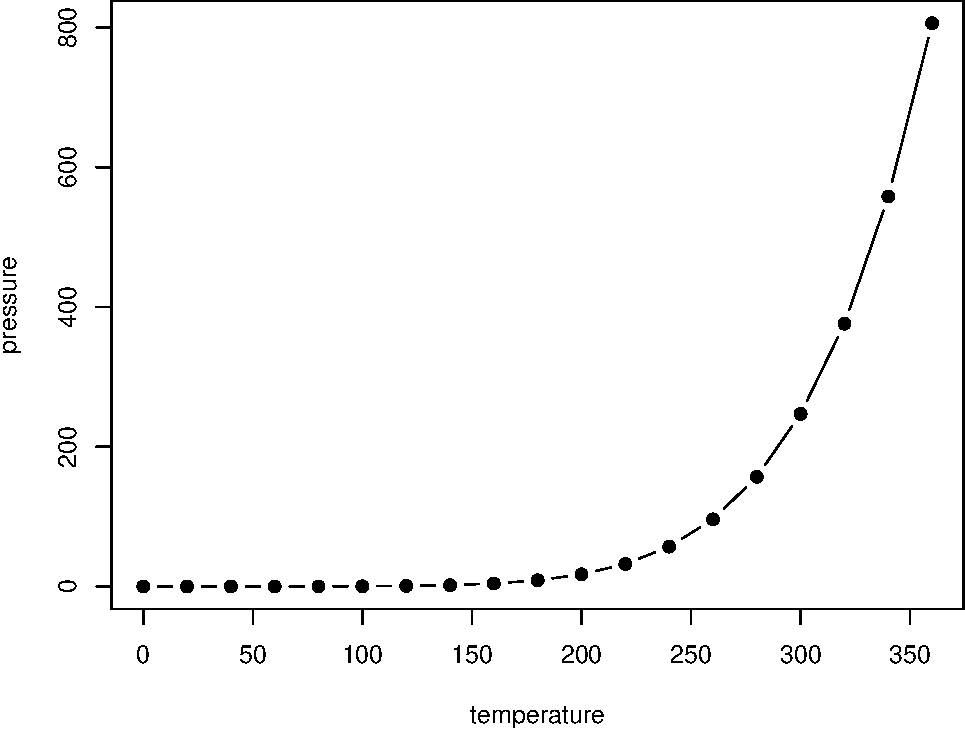
\includegraphics[width=0.8\linewidth]{BookR_files/figure-latex/nice-fig-1} 

}

\caption{Here is a nice figure!}\label{fig:nice-fig}
\end{figure}

Reference a figure by its code chunk label with the \texttt{fig:} prefix, e.g., see Figure \ref{fig:nice-fig}. Similarly, you can reference tables generated from \texttt{knitr::kable()}, e.g., see Table \ref{tab:nice-tab}.

\begin{Shaded}
\begin{Highlighting}[]
\NormalTok{knitr}\SpecialCharTok{::}\FunctionTok{kable}\NormalTok{(}
  \FunctionTok{head}\NormalTok{(iris, }\DecValTok{20}\NormalTok{), }\AttributeTok{caption =} \StringTok{\textquotesingle{}Here is a nice table!\textquotesingle{}}\NormalTok{,}
  \AttributeTok{booktabs =} \ConstantTok{TRUE}
\NormalTok{)}
\end{Highlighting}
\end{Shaded}

\begin{table}

\caption{\label{tab:nice-tab}Here is a nice table!}
\centering
\begin{tabular}[t]{rrrrl}
\toprule
Sepal.Length & Sepal.Width & Petal.Length & Petal.Width & Species\\
\midrule
5.1 & 3.5 & 1.4 & 0.2 & setosa\\
4.9 & 3.0 & 1.4 & 0.2 & setosa\\
4.7 & 3.2 & 1.3 & 0.2 & setosa\\
4.6 & 3.1 & 1.5 & 0.2 & setosa\\
5.0 & 3.6 & 1.4 & 0.2 & setosa\\
\addlinespace
5.4 & 3.9 & 1.7 & 0.4 & setosa\\
4.6 & 3.4 & 1.4 & 0.3 & setosa\\
5.0 & 3.4 & 1.5 & 0.2 & setosa\\
4.4 & 2.9 & 1.4 & 0.2 & setosa\\
4.9 & 3.1 & 1.5 & 0.1 & setosa\\
\addlinespace
5.4 & 3.7 & 1.5 & 0.2 & setosa\\
4.8 & 3.4 & 1.6 & 0.2 & setosa\\
4.8 & 3.0 & 1.4 & 0.1 & setosa\\
4.3 & 3.0 & 1.1 & 0.1 & setosa\\
5.8 & 4.0 & 1.2 & 0.2 & setosa\\
\addlinespace
5.7 & 4.4 & 1.5 & 0.4 & setosa\\
5.4 & 3.9 & 1.3 & 0.4 & setosa\\
5.1 & 3.5 & 1.4 & 0.3 & setosa\\
5.7 & 3.8 & 1.7 & 0.3 & setosa\\
5.1 & 3.8 & 1.5 & 0.3 & setosa\\
\bottomrule
\end{tabular}
\end{table}

You can write citations, too. For example, we are using the \textbf{bookdown} package \citep{R-bookdown} in this sample book, which was built on top of R Markdown and \textbf{knitr} \citep{xie2015}.

\hypertarget{marcos-de-datos-y-tibbles}{%
\chapter{Marcos de datos y Tibbles}\label{marcos-de-datos-y-tibbles}}

Cree estructuras de datos tabulares con marcos de datos y vea cómo se comparan con tibbles. Extraiga vectores de columna de marcos de datos para realizar cálculos. Obtenga información de metadatos como dimensiones. Seleccione las filas superior e inferior para obtener una descripción general rápida.

\hypertarget{construye-un-marco-de-datos-a-partir-de-vectores}{%
\section{Construye un marco de datos a partir de vectores}\label{construye-un-marco-de-datos-a-partir-de-vectores}}

Los datos tabulares son el formato más común utilizado por los científicos de datos. En R, las tablas se representan mediante marcos de datos. Pueden inspeccionarse imprimiéndolos en la consola.

\begin{itemize}
\tightlist
\item
  Comprender por qué los marcos de datos son importantes
\item
  Interpretar la salida de la consola creada por un marco de datos
\item
  Cree un nuevo marco de datos usando la función \texttt{data.frame()}
\item
  Definir los vectores que se utilizarán para columnas individuales
\item
  Especificar los nombres de las columnas del marco de datos
\end{itemize}

\begin{verbatim}
data.frame(___ = ___, 
           ___ = ___, 
           ...)
\end{verbatim}

\hypertarget{introducciuxf3n-a-los-marcos-de-datos}{%
\subsection{Introducción a los marcos de datos}\label{introducciuxf3n-a-los-marcos-de-datos}}

En análisis y estadísticas, los datos tabulares son la estructura de datos más importante. Está presente en muchos formatos comunes como archivos de Excel, valores separados por comas (CSV) o bases de datos. R integra objetos de datos tabulares como ciudadanos de primera clase en el idioma a través de \emph{marcos de datos}. Los marcos de datos permiten a los usuarios leer y manipular fácilmente datos tabulares dentro del lenguaje R.

Echemos un vistazo a un objeto de marco de datos llamado \texttt{Davis}, del paquete \textbf{carData}, que incluye medidas de altura y peso para 200 hombres y mujeres:

\begin{Shaded}
\begin{Highlighting}[]
\FunctionTok{tibble}\NormalTok{ (Davis)}
\end{Highlighting}
\end{Shaded}

\begin{verbatim}
## # A tibble: 200 x 5
##    sex   weight height repwt repht
##    <fct>  <int>  <int> <int> <int>
##  1 M         77    182    77   180
##  2 F         58    161    51   159
##  3 F         53    161    54   158
##  4 M         68    177    70   175
##  5 F         59    157    59   155
##  6 M         76    170    76   165
##  7 M         76    167    77   165
##  8 M         69    186    73   180
##  9 M         71    178    71   175
## 10 M         65    171    64   170
## # ... with 190 more rows
\end{verbatim}

De la salida impresa, podemos ver que el marco de datos abarca más de 200 \textbf{filas} y 5 \textbf{columnas}. En el ejemplo anterior, cada fila contiene datos de una persona a través de \textbf{atributos}, que corresponden a las columnas \texttt{sex}, \texttt{weight}, \texttt{height}, \texttt{repwt} (peso reportado) y \texttt{repht} (altura reportado).

Por ejemplo, la primera fila de la tabla especifica un hombre que pesa \texttt{77} kg y tiene una altura de \texttt{182} cm. Los pesos reportados están muy cerca de \texttt{77} kg y \texttt{180} cm, respectivamente.

Las filas en un marco de datos se identifican además por los \emph{nombres de fila} a la izquierda, que son simplemente los números de fila por defecto. En el caso del conjunto de datos de \texttt{Davis} anterior, los nombres de las filas van de 1 a 200.

\hypertarget{crear-marcos-de-datos}{%
\subsection{Crear marcos de datos}\label{crear-marcos-de-datos}}

\begin{verbatim}
data.frame(___ = ___, 
           ___ = ___, 
           ...)
\end{verbatim}

Los marcos de datos contienen datos tabulares en varias columnas o \emph{atributos}. Cada columna está representada por un vector de diferentes \emph{tipos de datos} como números o caracteres. La función \texttt{data.frame()} admite la construcción de objetos de marco de datos combinando diferentes vectores en una tabla. Para formar una tabla, se requiere que los vectores tengan la misma longitud. Un marco de datos también puede verse como una colección de vectores conectados entre sí para formar una tabla.

Creemos nuestro primer marco de datos con cuatro personas diferentes, incluidos sus identificadores, nombres e indicadores si son mujeres o no. Cada uno de estos atributos es creado por un vector diferente de diferentes tipos de datos (numéricos, de caracteres y lógicos). Los atributos finalmente se combinan en una tabla usando la función \texttt{data.frame()}:

\begin{Shaded}
\begin{Highlighting}[]
\FunctionTok{data.frame}\NormalTok{(}
  \FunctionTok{c}\NormalTok{(}\DecValTok{1}\NormalTok{, }\DecValTok{2}\NormalTok{, }\DecValTok{3}\NormalTok{, }\DecValTok{4}\NormalTok{),}
  \FunctionTok{c}\NormalTok{(}\StringTok{"Louisa"}\NormalTok{, }\StringTok{"Jonathan"}\NormalTok{, }\StringTok{"Luigi"}\NormalTok{, }\StringTok{"Rachel"}\NormalTok{),}
  \FunctionTok{c}\NormalTok{(}\ConstantTok{TRUE}\NormalTok{, }\ConstantTok{FALSE}\NormalTok{, }\ConstantTok{FALSE}\NormalTok{, }\ConstantTok{TRUE}\NormalTok{)}
\NormalTok{)}
\end{Highlighting}
\end{Shaded}

\begin{verbatim}
##   c.1..2..3..4. c..Louisa....Jonathan....Luigi....Rachel..
## 1             1                                     Louisa
## 2             2                                   Jonathan
## 3             3                                      Luigi
## 4             4                                     Rachel
##   c.TRUE..FALSE..FALSE..TRUE.
## 1                        TRUE
## 2                       FALSE
## 3                       FALSE
## 4                        TRUE
\end{verbatim}

El marco de datos resultante almacena los valores de cada vector en una columna diferente. Tiene cuatro filas y tres columnas. Sin embargo, los nombres de las columnas impresas en la primera línea parecen incluir los valores de las columnas separados por puntos, lo cual es un esquema de nombres muy extraño.

Los nombres de columna se pueden incluir en la construcción de \texttt{data.frame()} como nombres de argumentos que preceden a los valores de los vectores de columna. Para mejorar el nombre de la columna del marco de datos anterior, podemos escribir

\begin{Shaded}
\begin{Highlighting}[]
\FunctionTok{data.frame}\NormalTok{(}
  \AttributeTok{id =} \FunctionTok{c}\NormalTok{(}\DecValTok{1}\NormalTok{, }\DecValTok{2}\NormalTok{, }\DecValTok{3}\NormalTok{, }\DecValTok{4}\NormalTok{),}
  \AttributeTok{name =} \FunctionTok{c}\NormalTok{(}\StringTok{"Louisa"}\NormalTok{, }\StringTok{"Jonathan"}\NormalTok{, }\StringTok{"Luigi"}\NormalTok{, }\StringTok{"Rachel"}\NormalTok{),}
  \AttributeTok{female =} \FunctionTok{c}\NormalTok{(}\ConstantTok{TRUE}\NormalTok{, }\ConstantTok{FALSE}\NormalTok{, }\ConstantTok{FALSE}\NormalTok{, }\ConstantTok{TRUE}\NormalTok{)}
\NormalTok{)}
\end{Highlighting}
\end{Shaded}

\begin{verbatim}
##   id     name female
## 1  1   Louisa   TRUE
## 2  2 Jonathan  FALSE
## 3  3    Luigi  FALSE
## 4  4   Rachel   TRUE
\end{verbatim}

El marco de datos resultante incluye los nombres de columna necesarios para ver el significado real de las diferentes columnas.

\hypertarget{crea-y-convierte-tibbles}{%
\section{Crea y convierte tibbles}\label{crea-y-convierte-tibbles}}

Tibbles son la reimaginación moderna de marcos de datos y comparten muchos puntos en común con sus antepasados. La diferencia más visible es cómo se imprime el contenido de tibble en la consola. Tibbles son parte del tidyverse y se utilizan por su comportamiento más consistente en comparación con los marcos de datos.

\begin{itemize}
\tightlist
\item
  Conozca la diferencia entre \emph{marcos de datos} y \emph{tibbles}
\item
  Crear \emph{tibbles} a partir de vectores
\item
  Convertir \emph{marcos de datos} en tibbles
\end{itemize}

\begin{verbatim}
tibble(___ = ___, 
       ___ = ___, 
       ...)
as_tibble(___)
\end{verbatim}

\hypertarget{introducciuxf3n-a-tibbles}{%
\subsection{Introducción a Tibbles}\label{introducciuxf3n-a-tibbles}}

\begin{quote}
Una reinvención moderna del marco de datos
\url{https://tibble.tidyverse.org}
\end{quote}

Tibbles son en muchos aspectos similares a los marcos de datos. De hecho, se \emph{heredan} de los marcos de datos, lo que significa que todas las funciones y características disponibles para los marcos de datos también funcionan para tibbles. Por tanto, cuando hablamos de \emph{marcos de datos} también nos referimos a \emph{tibbles}.

Además de todo lo que ofrece un marco de datos, los tibbles tienen un comportamiento más consistente con una mejor usabilidad en muchos casos. Lo más importante es que cuando se imprime un objeto tibble en la consola, muestra automáticamente solo las primeras 10 filas y condensa columnas adicionales. Por el contrario, un marco de datos llena toda la pantalla de la consola con valores que pueden generar confusión. Echemos un vistazo al conjunto de datos \texttt{gapminder} del paquete \textbf{gapminder}:

\begin{Shaded}
\begin{Highlighting}[]
\NormalTok{gapminder}\SpecialCharTok{::}\NormalTok{gapminder}
\end{Highlighting}
\end{Shaded}

\begin{verbatim}
## # A tibble: 1,704 x 6
##    country     continent  year lifeExp      pop gdpPercap
##    <fct>       <fct>     <int>   <dbl>    <int>     <dbl>
##  1 Afghanistan Asia       1952    28.8  8425333      779.
##  2 Afghanistan Asia       1957    30.3  9240934      821.
##  3 Afghanistan Asia       1962    32.0 10267083      853.
##  4 Afghanistan Asia       1967    34.0 11537966      836.
##  5 Afghanistan Asia       1972    36.1 13079460      740.
##  6 Afghanistan Asia       1977    38.4 14880372      786.
##  7 Afghanistan Asia       1982    39.9 12881816      978.
##  8 Afghanistan Asia       1987    40.8 13867957      852.
##  9 Afghanistan Asia       1992    41.7 16317921      649.
## 10 Afghanistan Asia       1997    41.8 22227415      635.
## # ... with 1,694 more rows
\end{verbatim}

Inmediatamente vemos que el conjunto de datos \texttt{gapminder} es un tibble que consta de 1,704 filas y 6 columnas en la línea superior. En la segunda línea podemos ver los nombres de las columnas y sus correspondientes \emph{tipos de datos} directamente debajo.

Por ejemplo, la columna \texttt{country} tiene el tipo \texttt{\textless{}fct\textgreater{}} (que es la abreviatura de ``factor''), \texttt{year} es un número entero \texttt{\textless{}int\textgreater{}} y la esperanza de vida \texttt{lifeExp} es un \texttt{\textless{}dbl\textgreater{}}, un número decimal.

\hypertarget{creando-tibbles}{%
\subsection{Creando Tibbles}\label{creando-tibbles}}

\begin{verbatim}
tibble(___ = ___, 
       ___ = ___, 
       ...)
as_tibble(___)
\end{verbatim}

La creación de tibbles funciona exactamente igual que para los marcos de datos. Podemos usar la función \texttt{tibble()} del paquete \textbf{tibble} para crear un nuevo objeto tabular.

Por ejemplo, un tibble que contenga datos de cuatro personas diferentes y tres columnas se puede crear así:

\begin{Shaded}
\begin{Highlighting}[]
\FunctionTok{library}\NormalTok{(tibble)}
\FunctionTok{tibble}\NormalTok{(}
  \AttributeTok{id =} \FunctionTok{c}\NormalTok{(}\DecValTok{1}\NormalTok{, }\DecValTok{2}\NormalTok{, }\DecValTok{3}\NormalTok{, }\DecValTok{4}\NormalTok{),}
  \AttributeTok{name =} \FunctionTok{c}\NormalTok{(}\StringTok{"Louisa"}\NormalTok{, }\StringTok{"Jonathan"}\NormalTok{, }\StringTok{"Luigi"}\NormalTok{, }\StringTok{"Rachel"}\NormalTok{),}
  \AttributeTok{female =} \FunctionTok{c}\NormalTok{(}\ConstantTok{TRUE}\NormalTok{, }\ConstantTok{FALSE}\NormalTok{, }\ConstantTok{FALSE}\NormalTok{, }\ConstantTok{TRUE}\NormalTok{)}
\NormalTok{)}
\end{Highlighting}
\end{Shaded}

\begin{verbatim}
## # A tibble: 4 x 3
##      id name     female
##   <dbl> <chr>    <lgl> 
## 1     1 Louisa   TRUE  
## 2     2 Jonathan FALSE 
## 3     3 Luigi    FALSE 
## 4     4 Rachel   TRUE
\end{verbatim}

\hypertarget{conversiuxf3n-de-marcos-de-datos-a-tibbles}{%
\subsection{Conversión de marcos de datos a Tibbles}\label{conversiuxf3n-de-marcos-de-datos-a-tibbles}}

Si prefiere tibbles a marcos de datos por sus características adicionales, también se pueden convertir a partir de marcos de datos existentes con la función \texttt{as\_tibble()}.

Por ejemplo, el marco de datos de \texttt{Davis} del paquete \textbf{carData} se puede convertir a un tibble así:

\begin{Shaded}
\begin{Highlighting}[]
\FunctionTok{as\_tibble}\NormalTok{(Davis)}
\end{Highlighting}
\end{Shaded}

\begin{verbatim}
## # A tibble: 200 x 5
##    sex   weight height repwt repht
##    <fct>  <int>  <int> <int> <int>
##  1 M         77    182    77   180
##  2 F         58    161    51   159
##  3 F         53    161    54   158
##  4 M         68    177    70   175
##  5 F         59    157    59   155
##  6 M         76    170    76   165
##  7 M         76    167    77   165
##  8 M         69    186    73   180
##  9 M         71    178    71   175
## 10 M         65    171    64   170
## # ... with 190 more rows
\end{verbatim}

\hypertarget{extraiga-o-reemplace-columnas-en-un-marco-de-datos-usando}{%
\section{Extraiga o reemplace columnas en un marco de datos usando \$}\label{extraiga-o-reemplace-columnas-en-un-marco-de-datos-usando}}

Las columnas de un marco de datos se pueden extraer y manipular fácilmente con el operador \texttt{\$}. Incluso se pueden agregar nuevas columnas asignando un vector.

\begin{itemize}
\tightlist
\item
  Extraiga columnas de un marco de datos con \texttt{\$}.
\item
  Reemplazar valores de columnas existentes en un marco de datos.
\item
  Agregue nuevas columnas a un marco de datos.
\end{itemize}

\begin{verbatim}
___$___
___$___  <- ___
\end{verbatim}

\hypertarget{extraer-columnas-con}{%
\subsection{Extraer columnas con \$}\label{extraer-columnas-con}}

Los marcos de datos son tablas que resultan de la combinación de vectores de columna. Los usuarios pueden interactuar con los marcos de datos a través de numerosos operadores para extraer, agregar o recombinar valores. Para extraer columnas individuales de un marco de datos, R ofrece un operador muy específico: el dólar \texttt{\$}. Devuelve el vector de columna como lo indica su nombre basado en un marco de datos que precede a \texttt{\$}.

Para ver el operador \texttt{\$} en acción, extraigamos la población \texttt{pop} (en 1,000) de diferentes estados de los EE. UU. Según el conjunto de datos de los estados (de 1992) en el paquete \textbf{carData}:

\begin{Shaded}
\begin{Highlighting}[]
\NormalTok{carData}\SpecialCharTok{::}\NormalTok{States}\SpecialCharTok{$}\NormalTok{pop}
\end{Highlighting}
\end{Shaded}

\begin{verbatim}
##  [1]  4041   550  3665  2351 29760  3294  3287   666   607 12938  6478  1108
## [13]  1007 11431  5544  2777  2478  3685  4220  1228  4781  6016  9295  4375
## [25]  2573  5117   799  1578  1202  1109  7730  1515 17990  6629   639 10847
## [37]  3146  2842 11882  1003  3487   696  4877 16987  1723   563  6187  4867
## [49]  1793  4892   454
\end{verbatim}

El comando extrae la columna de población como vector del marco de datos. A partir de este vector podemos calcular la \texttt{sum()} de la población total como:

\begin{Shaded}
\begin{Highlighting}[]
\FunctionTok{sum}\NormalTok{(States}\SpecialCharTok{$}\NormalTok{pop)}
\end{Highlighting}
\end{Shaded}

\begin{verbatim}
## [1] 248709
\end{verbatim}

De manera similar, el salario promedio (en \$1,000) de los maestros se puede calcular como la \texttt{mean()} de la columna \texttt{pay}:

\begin{Shaded}
\begin{Highlighting}[]
\FunctionTok{mean}\NormalTok{(States}\SpecialCharTok{$}\NormalTok{pay)}
\end{Highlighting}
\end{Shaded}

\begin{verbatim}
## [1] 30.94118
\end{verbatim}

\hypertarget{determinar-el-tamauxf1o-de-un-marco-de-datos}{%
\section{Determinar el tamaño de un marco de datos}\label{determinar-el-tamauxf1o-de-un-marco-de-datos}}

El tamaño de un marco de datos, como el número de filas o columnas, a menudo es necesario y se puede determinar de varias formas.

\begin{itemize}
\tightlist
\item
  Obtener el número de filas de un marco de datos
\item
  Obtener el número de columnas de un marco de datos
\item
  Obtener dimensiones de un marco de datos
\end{itemize}

\begin{verbatim}
nrow(___)
ncol(___)
dim(___)
length(___)
\end{verbatim}

\hypertarget{dimensiones-del-marco-de-datos}{%
\subsection{Dimensiones del marco de datos}\label{dimensiones-del-marco-de-datos}}

El número de filas y columnas en un marco de datos se puede adivinar a través de la salida impresa del marco de datos. Sin embargo, es mucho más fácil obtener esta información directamente a través de funciones. Además, es posible que desee utilizar esta información en algunas partes del código.

Los marcos de datos tienen dos dimensiones. El número de filas se considera la primera dimensión. Por lo general, define el número de observaciones en un conjunto de datos. Para obtener el número de filas del marco de datos de \texttt{Davis} en el conjunto de datos \textbf{carData}, use la función \texttt{nrow()}:

\begin{Shaded}
\begin{Highlighting}[]
\FunctionTok{nrow}\NormalTok{(Davis)}
\end{Highlighting}
\end{Shaded}

\begin{verbatim}
## [1] 200
\end{verbatim}

De manera similar, el número de columnas o \emph{atributos} del marco de datos se puede recuperar con \texttt{ncol()}:

\begin{Shaded}
\begin{Highlighting}[]
\FunctionTok{ncol}\NormalTok{(Davis)}
\end{Highlighting}
\end{Shaded}

\begin{verbatim}
## [1] 5
\end{verbatim}

\hypertarget{recuperar-las-dimensiones-del-marco-de-datos}{%
\subsection{Recuperar las dimensiones del marco de datos}\label{recuperar-las-dimensiones-del-marco-de-datos}}

Para recuperar el tamaño de todas las dimensiones de un marco de datos a la vez, puede usar la función \texttt{dim()}. \texttt{dim()} devuelve un vector con dos elementos, el primer elemento es el número de filas y el segundo elemento el número de columnas.

Por ejemplo, las dimensiones del conjunto de datos de \texttt{Davis} se pueden recuperar como:

\begin{Shaded}
\begin{Highlighting}[]
\FunctionTok{dim}\NormalTok{(Davis)}
\end{Highlighting}
\end{Shaded}

\begin{verbatim}
## [1] 200   5
\end{verbatim}

Además de los marcos de datos, \texttt{dim()} también se puede utilizar para otros objetos R multidimensionales, como matrices. Sin embargo, cuando se usa con vectores \texttt{dim} solo devuelve \texttt{NULL}:

\begin{Shaded}
\begin{Highlighting}[]
\FunctionTok{dim}\NormalTok{(}\FunctionTok{c}\NormalTok{(}\DecValTok{1}\NormalTok{, }\DecValTok{3}\NormalTok{, }\DecValTok{5}\NormalTok{, }\DecValTok{7}\NormalTok{))}
\end{Highlighting}
\end{Shaded}

\begin{verbatim}
## NULL
\end{verbatim}

En cambio, la longitud de un vector se determina mediante \texttt{length()}:

\begin{Shaded}
\begin{Highlighting}[]
\FunctionTok{length}\NormalTok{(}\FunctionTok{c}\NormalTok{(}\DecValTok{1}\NormalTok{, }\DecValTok{3}\NormalTok{, }\DecValTok{5}\NormalTok{, }\DecValTok{7}\NormalTok{))}
\end{Highlighting}
\end{Shaded}

\begin{verbatim}
## [1] 4
\end{verbatim}

En el caso de un marco de datos, \texttt{length()} devuelve su número de columnas:

\begin{Shaded}
\begin{Highlighting}[]
\FunctionTok{length}\NormalTok{(Davis)}
\end{Highlighting}
\end{Shaded}

\begin{verbatim}
## [1] 5
\end{verbatim}

\hypertarget{seleccionar-la-primera-o-la-uxfaltima-fila-de-un-marco-de-datos}{%
\section{Seleccionar la primera o la última fila de un marco de datos}\label{seleccionar-la-primera-o-la-uxfaltima-fila-de-un-marco-de-datos}}

A menudo no necesitamos mirar todo el contenido de un marco de datos en la consola. En cambio, solo algunas partes son suficientes, como la parte superior o inferior recuperada a través de las funciones \texttt{head()} y \texttt{tail()}.

\begin{itemize}
\tightlist
\item
  Seleccionar la parte superior de un marco de datos
\item
  Seleccione la parte inferior de un marco de datos
\item
  Especifique el número de líneas a seleccionar mediante el parámetro n
\end{itemize}

\begin{verbatim}
head(___, n = ___)
tail(___, n = ___)
\end{verbatim}

\hypertarget{seleccionar-la-parte-superior-de-un-marco-de-datos}{%
\subsection{Seleccionar la parte superior de un marco de datos}\label{seleccionar-la-parte-superior-de-un-marco-de-datos}}

Los marcos de datos pueden abarcar una gran cantidad de filas y columnas. Según la salida impresa en la consola, puede ser difícil obtener una impresión inicial de los datos dentro del marco de datos. Este problema no es tanto un problema para tibbles que tienen una mejor salida de consola. Además, puede ser útil recuperar fácilmente las primeras filas en un comando sin indexación ni paquetes adicionales.

El conjunto de datos \texttt{TitanicSurvival} contiene datos de 1309 pasajeros representados como filas. Una simple impresión del conjunto de datos imprimiría a todos los pasajeros, llenando toda la consola. En cambio, la función \texttt{head()} muestra solo las primeras 10 filas de un marco de datos, incluidos los nombres de sus columnas:

\begin{Shaded}
\begin{Highlighting}[]
\FunctionTok{head}\NormalTok{(TitanicSurvival)}
\end{Highlighting}
\end{Shaded}

\begin{verbatim}
##                                 survived    sex     age passengerClass
## Allen, Miss. Elisabeth Walton        yes female 29.0000            1st
## Allison, Master. Hudson Trevor       yes   male  0.9167            1st
## Allison, Miss. Helen Loraine          no female  2.0000            1st
## Allison, Mr. Hudson Joshua Crei       no   male 30.0000            1st
## Allison, Mrs. Hudson J C (Bessi       no female 25.0000            1st
## Anderson, Mr. Harry                  yes   male 48.0000            1st
\end{verbatim}

El número de columnas se puede ajustar mediante el parámetro \texttt{n}. Para extraer solo las primeras tres filas del conjunto de datos, puede escribir:

\begin{Shaded}
\begin{Highlighting}[]
\FunctionTok{head}\NormalTok{(TitanicSurvival, }\AttributeTok{n =} \DecValTok{3}\NormalTok{)}
\end{Highlighting}
\end{Shaded}

\begin{verbatim}
##                                survived    sex     age passengerClass
## Allen, Miss. Elisabeth Walton       yes female 29.0000            1st
## Allison, Master. Hudson Trevor      yes   male  0.9167            1st
## Allison, Miss. Helen Loraine         no female  2.0000            1st
\end{verbatim}

\hypertarget{seleccionar-la-parte-inferior-de-un-marco-de-datos}{%
\subsection{Seleccionar la parte inferior de un marco de datos}\label{seleccionar-la-parte-inferior-de-un-marco-de-datos}}

La función \texttt{tail()} se puede utilizar para seleccionar las filas inferiores de un marco de datos. Similar a la función \texttt{head()}, también acepta un parámetro \texttt{n} para especificar el número de filas que se devolverán.

Por ejemplo, para seleccionar las últimas cinco filas del conjunto de datos \texttt{TitanicSurvival}, puede escribir:

\begin{Shaded}
\begin{Highlighting}[]
\FunctionTok{tail}\NormalTok{(TitanicSurvival, }\AttributeTok{n =} \DecValTok{5}\NormalTok{)}
\end{Highlighting}
\end{Shaded}

\begin{verbatim}
##                           survived    sex  age passengerClass
## Zabour, Miss. Hileni            no female 14.5            3rd
## Zabour, Miss. Thamine           no female   NA            3rd
## Zakarian, Mr. Mapriededer       no   male 26.5            3rd
## Zakarian, Mr. Ortin             no   male 27.0            3rd
## Zimmerman, Mr. Leo              no   male 29.0            3rd
\end{verbatim}

Las funciones de cabeza y cola también se pueden combinar para seleccionar un fragmento del conjunto de datos del medio. Para seleccionar las primeras cinco filas de las 500 filas inferiores, puede escribir:

\begin{Shaded}
\begin{Highlighting}[]
\FunctionTok{head}\NormalTok{(}\FunctionTok{tail}\NormalTok{(TitanicSurvival, }\AttributeTok{n =} \DecValTok{500}\NormalTok{), }\AttributeTok{n =} \DecValTok{5}\NormalTok{)}
\end{Highlighting}
\end{Shaded}

\begin{verbatim}
##                                 survived    sex age passengerClass
## Ford, Mr. Edward Watson               no   male  18            3rd
## Ford, Mr. William Neal                no   male  16            3rd
## Ford, Mrs. Edward (Margaret Ann       no female  48            3rd
## Fox, Mr. Patrick                      no   male  NA            3rd
## Franklin, Mr. Charles (Charles        no   male  NA            3rd
\end{verbatim}

\hypertarget{transformaciuxf3n-de-datos-con-dplyr}{%
\chapter{Transformación de datos con dplyr}\label{transformaciuxf3n-de-datos-con-dplyr}}

Utilice verbos \texttt{dplyr} básicos para filtrar filas, seleccionar columnas y ordenar/organizar conjuntos de datos en combinación con el operador pipe \texttt{\%\textgreater{}\%}.

\hypertarget{introducciuxf3n-a-dplyr}{%
\section{Introducción a dplyr}\label{introducciuxf3n-a-dplyr}}

\textbf{dplyr} facilita el proceso de transformación de datos al proporcionar un marco enriquecido para manipular marcos de datos. Las funciones de \textbf{dplyr} se pueden concatenar a potentes canalizaciones de transformación para \emph{seleccionar}, \emph{filtrar}, \emph{ordenar}, \emph{unir} y \emph{agregar} datos.

\begin{itemize}
\tightlist
\item
  Descubra lo que hace \textbf{dplyr}
\item
  Obtenga una descripción general de Seleccionar, Filtrar y Ordenar
\item
  Descubra qué son las uniones, agregaciones y canalizaciones
\end{itemize}

\hypertarget{quuxe9-es-dplyr}{%
\subsection{¿Qué es dplyr?}\label{quuxe9-es-dplyr}}

\begin{quote}
Existe la broma de que el 80 \% de la ciencia de datos está limpiando los datos y el 20 \% se queja de limpiar los datos.
--- Anthony Goldbloom, fundador y CEO de Kaggle
\end{quote}

Tener datos \emph{limpios} en cualquier proyecto de Data Science es muy importante, porque los resultados solo son tan buenos como los datos correctos. La limpieza de datos también es la parte que generalmente consume la mayor parte del tiempo y causa los mayores dolores para los científicos de datos. R ya ofrece un amplio conjunto de herramientas y funciones para manipular marcos de datos. Sin embargo, debido a su larga historia, el conjunto de herramientas base R disponible está fragmentado y es difícil de usar para nuevos usuarios.

El paquete \textbf{dplyr} facilita el proceso de transformación de datos a través de una colección consistente de funciones. Estas funciones admiten diferentes transformaciones en marcos de datos, que incluyen

\begin{itemize}
\tightlist
\item
  filtrar filas
\item
  seleccionar columnas
\item
  ordenar datos
\item
  agregar datos
\end{itemize}

Múltiples marcos de datos también se pueden unir mediante valores de atributo comunes.

La coherencia de las funciones de \textbf{dplyr} mejora la usabilidad y permite al usuario conectar transformaciones para formar \emph{canalizaciones de datos}. Estas canalizaciones también se pueden ver como un lenguaje de consulta de alto nivel, como p.~Ej. el lenguaje SQL para consultas de bases de datos. Además, incluso es posible traducir las canalizaciones de datos creadas a otros back-end, incluidas las bases de datos.

\hypertarget{marco-de-funciones}{%
\subsection{Marco de funciones}\label{marco-de-funciones}}

Cada función de transformación de datos en \textbf{dplyr} acepta un marco de datos como su primer parámetro de entrada y devuelve el marco de datos transformado como salida. Un plano para una función \textbf{dplyr} típica se ve así:

\begin{Shaded}
\begin{Highlighting}[]
\NormalTok{transformed }\OtherTok{\textless{}{-}} \FunctionTok{dplyr\_function}\NormalTok{(my\_data\_frame, }
\NormalTok{                              param\_one, }
\NormalTok{                              param\_two, }
\NormalTok{                              ...)}
\end{Highlighting}
\end{Shaded}

La función \texttt{dplyr\_function} se puede personalizar aún más a través de argumentos adicionales (\texttt{param\_one}, \texttt{param\_two}) colocados después del primer parámetro de marco de datos (\texttt{my\_data\_frame}).

El poder real de \textbf{dplyr} viene con el operador pipe \texttt{\%\textgreater{}\%} que permite a los usuarios concatenar funciones de \textbf{dplyr} a pipe de datos. Pipe inyecta el marco de datos resultante del cálculo anterior como primer argumento del siguiente. Una transformación de datos que consta de tres funciones se parece a:

\begin{Shaded}
\begin{Highlighting}[]
\FunctionTok{dplyr\_function\_three}\NormalTok{(}
  \FunctionTok{dplyr\_function\_two}\NormalTok{(}
    \FunctionTok{dplyr\_function\_one}\NormalTok{(input\_data\_frame)))}
\end{Highlighting}
\end{Shaded}

pero con \texttt{pipe} se puede escribir de la siguiente manera:

\begin{Shaded}
\begin{Highlighting}[]
\NormalTok{input\_data\_frame }\SpecialCharTok{\%\textgreater{}\%}
  \FunctionTok{dplyr\_function\_one}\NormalTok{() }\SpecialCharTok{\%\textgreater{}\%}
  \FunctionTok{dplyr\_function\_two}\NormalTok{() }\SpecialCharTok{\%\textgreater{}\%}
  \FunctionTok{dplyr\_function\_three}\NormalTok{()}
\end{Highlighting}
\end{Shaded}

El orden de lectura diferente de las funciones de transformación de datos en el orden de transformación real, hace que las canalizaciones sean más fáciles de leer que las llamadas a funciones anidadas.

\hypertarget{seleccionar-columnas-de-un-marco-de-datos}{%
\section{Seleccionar columnas de un marco de datos}\label{seleccionar-columnas-de-un-marco-de-datos}}

Para seleccionar sólo un conjunto específico de columnas de marcos de datos interesantes, \textbf{dplyr} ofrece la función \texttt{select()} para extraer columnas por nombres, índices y rangos. Incluso puede renombrar las columnas extraídas con \texttt{select()}.

\begin{itemize}
\tightlist
\item
  Aprenda a usar la función \texttt{select()}
\item
  Seleccionar las columnas de un marco de datos por nombre o índice
\item
  Renombrar las columnas de un marco de datos
\end{itemize}

\begin{Shaded}
\begin{Highlighting}[]
\FunctionTok{select}\NormalTok{(my\_data\_frame, column\_one, column\_two, ...)}
\FunctionTok{select}\NormalTok{(my\_data\_frame, }\AttributeTok{new\_column\_name =}\NormalTok{ current\_column, ...)}
\FunctionTok{select}\NormalTok{(my\_data\_frame, column\_start}\SpecialCharTok{:}\NormalTok{column\_end)}
\FunctionTok{select}\NormalTok{(my\_data\_frame, index\_one, index\_two, ...)}
\FunctionTok{select}\NormalTok{(my\_data\_frame, index\_start}\SpecialCharTok{:}\NormalTok{index\_end)}
\end{Highlighting}
\end{Shaded}

\hypertarget{seleccionando-por-nombre}{%
\subsection{Seleccionando por nombre}\label{seleccionando-por-nombre}}

\begin{Shaded}
\begin{Highlighting}[]
\FunctionTok{select}\NormalTok{(my\_data\_frame, column\_one, column\_two, ...)}
\end{Highlighting}
\end{Shaded}

En este capítulo veremos el conjunto de datos \texttt{pres\_results} del paquete \textbf{politicaldata}. Contiene datos sobre las elecciones presidenciales de EE.UU. desde 1976, convertidas en un Tibble para una mejor impresión.

\begin{verbatim}
## # A tibble: 561 x 6
##     year state total_votes   dem   rep   other
##    <dbl> <chr>       <dbl> <dbl> <dbl>   <dbl>
##  1  1976 AK         123574 0.357 0.579 0.0549 
##  2  1976 AL        1182850 0.557 0.426 0.0163 
##  3  1976 AR         767535 0.650 0.349 0.00134
##  4  1976 AZ         742719 0.398 0.564 0.0383 
##  5  1976 CA        7803770 0.480 0.497 0.0230 
##  6  1976 CO        1081440 0.426 0.540 0.0336 
##  7  1976 CT        1386355 0.467 0.519 0.0138 
##  8  1976 DC         168830 0.816 0.165 0.0169 
##  9  1976 DE         235642 0.520 0.466 0.0144 
## 10  1976 FL        3150631 0.519 0.466 0.0143 
## # ... with 551 more rows
\end{verbatim}

Para este ejemplo, veremos el número total de votos en diferentes estados en diferentes elecciones. Como solo estamos interesados en la cantidad de personas que votaron, nos gustaría crear una versión personalizada del marco de datos \texttt{pres\_results} que solo contenga las columnas \texttt{year}, \texttt{state} y \texttt{total\_votes}. Para dicho filtrado, podemos usar la función \texttt{select()} del paquete \textbf{dplyr}.

La función \texttt{select()} toma un marco de datos como parámetro de entrada y nos permite decidir cuál de las columnas queremos mantener. El resultado de la función es un marco de datos con todas las filas, pero que contiene solo las columnas que seleccionamos explícitamente.

Podemos reducir nuestro conjunto de datos a solo \texttt{year}, \texttt{state} y \texttt{total\_votes} de la siguiente manera:

\begin{Shaded}
\begin{Highlighting}[]
\FunctionTok{tibble}\NormalTok{(}
\FunctionTok{select}\NormalTok{(pres\_results, year, state, total\_votes)}
\NormalTok{)}
\end{Highlighting}
\end{Shaded}

\begin{verbatim}
## # A tibble: 561 x 3
##     year state total_votes
##    <dbl> <chr>       <dbl>
##  1  1976 AK         123574
##  2  1976 AL        1182850
##  3  1976 AR         767535
##  4  1976 AZ         742719
##  5  1976 CA        7803770
##  6  1976 CO        1081440
##  7  1976 CT        1386355
##  8  1976 DC         168830
##  9  1976 DE         235642
## 10  1976 FL        3150631
## # ... with 551 more rows
\end{verbatim}

Como primer parámetro pasamos el marco de datos \texttt{pres\_results}, como parámetros restantes pasamos las columnas que queremos mantener para \texttt{select()}.

Además de mantener las columnas que queremos, la función \texttt{select()} también las mantiene en el mismo orden que especificamos en los parámetros de la función.

Si cambiamos el orden de los parámetros cuando llamamos a la función, las columnas de la salida cambian en consecuencia:

\begin{Shaded}
\begin{Highlighting}[]
\FunctionTok{tibble}\NormalTok{(}
\FunctionTok{select}\NormalTok{(pres\_results, total\_votes, year, state)}
\NormalTok{)}
\end{Highlighting}
\end{Shaded}

\begin{verbatim}
## # A tibble: 561 x 3
##    total_votes  year state
##          <dbl> <dbl> <chr>
##  1      123574  1976 AK   
##  2     1182850  1976 AL   
##  3      767535  1976 AR   
##  4      742719  1976 AZ   
##  5     7803770  1976 CA   
##  6     1081440  1976 CO   
##  7     1386355  1976 CT   
##  8      168830  1976 DC   
##  9      235642  1976 DE   
## 10     3150631  1976 FL   
## # ... with 551 more rows
\end{verbatim}

\hypertarget{renombrar-nombres-de-columnas}{%
\subsection{Renombrar nombres de columnas}\label{renombrar-nombres-de-columnas}}

\begin{Shaded}
\begin{Highlighting}[]
\FunctionTok{select}\NormalTok{(my\_data\_frame, }\AttributeTok{new\_column\_name =}\NormalTok{ current\_column, ...)}
\end{Highlighting}
\end{Shaded}

Además de definir las columnas que queremos conservar, también podemos cambiarles el nombre. Para hacer esto, necesitamos establecer el nuevo nombre de columna dentro de la función \texttt{select()} usando el comando

\begin{Shaded}
\begin{Highlighting}[]
\NormalTok{new\_column\_name }\OtherTok{=}\NormalTok{ current\_column}
\end{Highlighting}
\end{Shaded}

En el siguiente ejemplo, seleccionamos las columnas \texttt{year}, \texttt{state} y \texttt{total\_votes} pero cambiamos el nombre de la columna \texttt{year} a \texttt{Election} en la salida:

\begin{Shaded}
\begin{Highlighting}[]
\FunctionTok{tibble}\NormalTok{(}
\FunctionTok{select}\NormalTok{(pres\_results, }\AttributeTok{Election =}\NormalTok{ year, state, total\_votes)}
\NormalTok{)}
\end{Highlighting}
\end{Shaded}

\begin{verbatim}
## # A tibble: 561 x 3
##    Election state total_votes
##       <dbl> <chr>       <dbl>
##  1     1976 AK         123574
##  2     1976 AL        1182850
##  3     1976 AR         767535
##  4     1976 AZ         742719
##  5     1976 CA        7803770
##  6     1976 CO        1081440
##  7     1976 CT        1386355
##  8     1976 DC         168830
##  9     1976 DE         235642
## 10     1976 FL        3150631
## # ... with 551 more rows
\end{verbatim}

\hypertarget{selecciuxf3n-por-rango-de-nombre}{%
\subsection{Selección por rango de nombre}\label{selecciuxf3n-por-rango-de-nombre}}

\begin{Shaded}
\begin{Highlighting}[]
\FunctionTok{select}\NormalTok{(my\_data\_frame, column\_start}\SpecialCharTok{:}\NormalTok{column\_end)}
\end{Highlighting}
\end{Shaded}

Cuando usamos la función \texttt{select()} y definimos las columnas que queremos mantener, \textbf{dplyr} en realidad no usa el nombre de las columnas sino el índice de las columnas en el marco de datos. Esto significa que, cuando definimos las primeras tres columnas del marco de datos \texttt{pres\_results}, \texttt{year}, \texttt{state} y \texttt{total\_votes}, \textbf{dplyr} convierte estos nombres en los valores de índice \texttt{1}, \texttt{2} y \texttt{3}. Por lo tanto, también podemos usar el nombre de las columnas, aplicar el operador \texttt{:} y definir rangos de columnas, que queremos mantener:

\begin{Shaded}
\begin{Highlighting}[]
\FunctionTok{tibble}\NormalTok{(}
\FunctionTok{select}\NormalTok{(pres\_results, year}\SpecialCharTok{:}\NormalTok{total\_votes)}
\NormalTok{)}
\end{Highlighting}
\end{Shaded}

\begin{verbatim}
## # A tibble: 561 x 3
##     year state total_votes
##    <dbl> <chr>       <dbl>
##  1  1976 AK         123574
##  2  1976 AL        1182850
##  3  1976 AR         767535
##  4  1976 AZ         742719
##  5  1976 CA        7803770
##  6  1976 CO        1081440
##  7  1976 CT        1386355
##  8  1976 DC         168830
##  9  1976 DE         235642
## 10  1976 FL        3150631
## # ... with 551 more rows
\end{verbatim}

Lo que hace \texttt{year:total\_votes}, se puede traducir a \texttt{1:3}, que es simplemente crear un vector de valores numéricos del 1 al 3. Luego, la función \texttt{select()} toma el marco de datos \texttt{pres\_results} y genera un subconjunto del mismo, manteniendo solo Las primeras tres columnas.

\hypertarget{select-por-uxedndices}{%
\subsection{Select() por índices}\label{select-por-uxedndices}}

\begin{Shaded}
\begin{Highlighting}[]
\FunctionTok{select}\NormalTok{(my\_data\_frame, index\_one, index\_two, ...)}
\FunctionTok{select}\NormalTok{(my\_data\_frame, index\_start}\SpecialCharTok{:}\NormalTok{index\_end)}
\end{Highlighting}
\end{Shaded}

La función \texttt{select()} también se puede usar con índices de columna. En lugar de usar nombres, debemos especificar las columnas que queremos seleccionar por sus índices. En comparación con otros lenguajes de programación, la indexación en R comienza con \emph{uno} en lugar de \emph{cero}. Para seleccionar la primera, cuarta y quinta columna del conjunto de datos \texttt{pres\_results} podemos escribir

\begin{Shaded}
\begin{Highlighting}[]
\FunctionTok{tibble}\NormalTok{(}
\FunctionTok{select}\NormalTok{(pres\_results, }\DecValTok{1}\NormalTok{,}\DecValTok{4}\NormalTok{,}\DecValTok{5}\NormalTok{)}
\NormalTok{)}
\end{Highlighting}
\end{Shaded}

\begin{verbatim}
## # A tibble: 561 x 3
##     year   dem   rep
##    <dbl> <dbl> <dbl>
##  1  1976 0.357 0.579
##  2  1976 0.557 0.426
##  3  1976 0.650 0.349
##  4  1976 0.398 0.564
##  5  1976 0.480 0.497
##  6  1976 0.426 0.540
##  7  1976 0.467 0.519
##  8  1976 0.816 0.165
##  9  1976 0.520 0.466
## 10  1976 0.519 0.466
## # ... with 551 more rows
\end{verbatim}

De manera similar a la definición de rangos de columnas usando sus nombres, podemos definir rangos (o vectores) de valores de índice en su lugar:

\begin{Shaded}
\begin{Highlighting}[]
\FunctionTok{tibble}\NormalTok{(}
\FunctionTok{select}\NormalTok{(pres\_results, }\DecValTok{1}\SpecialCharTok{:}\DecValTok{3}\NormalTok{)}
\NormalTok{)}
\end{Highlighting}
\end{Shaded}

\begin{verbatim}
## # A tibble: 561 x 3
##     year state total_votes
##    <dbl> <chr>       <dbl>
##  1  1976 AK         123574
##  2  1976 AL        1182850
##  3  1976 AR         767535
##  4  1976 AZ         742719
##  5  1976 CA        7803770
##  6  1976 CO        1081440
##  7  1976 CT        1386355
##  8  1976 DC         168830
##  9  1976 DE         235642
## 10  1976 FL        3150631
## # ... with 551 more rows
\end{verbatim}

\hypertarget{filtrar-filas-de-marcos-de-datos}{%
\section{Filtrar filas de marcos de datos}\label{filtrar-filas-de-marcos-de-datos}}

A menudo queremos operar sólo en un subconjunto específico de filas de un marco de datos. La función \textbf{dplyr} \texttt{filter()} proporciona una forma flexible de extraer las filas de interés en base a múltiples condiciones.

\begin{itemize}
\tightlist
\item
  Utilice la función \texttt{filter()} para ordenar las filas de un marco de datos que cumplan una condición específica
\item
  Filtrar un cuadro de datos por múltiples condiciones
\end{itemize}

\begin{Shaded}
\begin{Highlighting}[]
\FunctionTok{filter}\NormalTok{(my\_data\_frame, condition)}
\FunctionTok{filter}\NormalTok{(my\_data\_frame, condition\_one, condition\_two, ...)}
\end{Highlighting}
\end{Shaded}

\hypertarget{funciuxf3n-filter}{%
\subsection{Función filter()}\label{funciuxf3n-filter}}

\begin{Shaded}
\begin{Highlighting}[]
\FunctionTok{filter}\NormalTok{(my\_data\_frame, condition)}
\end{Highlighting}
\end{Shaded}

La función \texttt{filter()} toma un marco de datos y una o más expresiones de filtrado como parámetros de entrada. Procesa el marco de datos y mantiene solo las filas que cumplen con las expresiones de filtrado definidas. Estas expresiones pueden verse como reglas para la evaluación y el mantenimiento de filas. En la mayoría de los casos, se basan en operadores relacionales. Como ejemplo, podríamos filtrar el marco de datos \texttt{pres\_results} y mantener solo las filas, donde la variable de \texttt{state} es igual a \texttt{"CA"} (California):

\begin{Shaded}
\begin{Highlighting}[]
\FunctionTok{tibble}\NormalTok{(}
\FunctionTok{filter}\NormalTok{(pres\_results, state }\SpecialCharTok{==} \StringTok{"CA"}\NormalTok{)}
\NormalTok{)}
\end{Highlighting}
\end{Shaded}

\begin{verbatim}
## # A tibble: 11 x 6
##     year state total_votes   dem   rep  other
##    <dbl> <chr>       <dbl> <dbl> <dbl>  <dbl>
##  1  1976 CA        7803770 0.480 0.497 0.0230
##  2  1980 CA        8582938 0.359 0.527 0.114 
##  3  1984 CA        9505041 0.413 0.575 0.0122
##  4  1988 CA        9887065 0.476 0.511 0.0131
##  5  1992 CA       11131721 0.460 0.326 0.213 
##  6  1996 CA       10019469 0.511 0.382 0.107 
##  7  2000 CA       10965822 0.534 0.417 0.0490
##  8  2004 CA       12421353 0.543 0.444 0.0117
##  9  2008 CA       13561900 0.610 0.370 0.0188
## 10  2012 CA       13038547 0.602 0.371 0.0246
## 11  2016 CA       14181595 0.617 0.316 0.0581
\end{verbatim}

En el resultado, podemos comparar los resultados de las elecciones en California para diferentes años.

Como otro ejemplo, podríamos filtrar el marco de datos \texttt{pres\_results} y mantener solo aquellas filas, donde la variable \texttt{dem} (porcentaje de votos para el Partido Demócrata) es mayor que 0.85:

\begin{Shaded}
\begin{Highlighting}[]
\FunctionTok{tibble}\NormalTok{(}
\FunctionTok{filter}\NormalTok{(pres\_results, dem }\SpecialCharTok{\textgreater{}} \FloatTok{0.85}\NormalTok{)}
\NormalTok{)}
\end{Highlighting}
\end{Shaded}

\begin{verbatim}
## # A tibble: 7 x 6
##    year state total_votes   dem    rep   other
##   <dbl> <chr>       <dbl> <dbl>  <dbl>   <dbl>
## 1  1984 DC         211288 0.854 0.137  0.00886
## 2  1996 DC         185726 0.852 0.0934 0.0513 
## 3  2000 DC         201894 0.852 0.0895 0.0563 
## 4  2004 DC         227586 0.892 0.0934 0.0125 
## 5  2008 DC         265853 0.925 0.0653 0.00582
## 6  2012 DC         293764 0.909 0.0728 0.0155 
## 7  2016 DC         312575 0.905 0.0407 0.0335
\end{verbatim}

En el resultado podemos ver para cada año electoral los estados donde el Partido Demócrata obtuvo más del 85\% de los votos. Según los resultados, podríamos decir que el Partido Demócrata tiene una base sólida de votantes en el Distrito de Columbia (conocido como Washington, D.C.).

\hypertarget{muxfaltiples-expresiones-de-filtro}{%
\subsection{Múltiples expresiones de filtro}\label{muxfaltiples-expresiones-de-filtro}}

\begin{Shaded}
\begin{Highlighting}[]
\FunctionTok{filter}\NormalTok{(my\_data\_frame, condition\_one, condition\_two, ...)}
\end{Highlighting}
\end{Shaded}

La función \texttt{filter()} también puede tomar múltiples reglas de filtrado como entrada. Estos pueden verse como una combinación de reglas con el operador \texttt{\&}. Para que una fila se incluya en la salida, todas las reglas de filtrado deben cumplirse. En el siguiente ejemplo, filtramos el marco de datos \texttt{pres\_results} para todas las filas donde la variable \texttt{state} es igual a \texttt{"CA"} y la variable de \texttt{year} es igual a 2016:

\begin{Shaded}
\begin{Highlighting}[]
\FunctionTok{tibble}\NormalTok{(}
\FunctionTok{filter}\NormalTok{(pres\_results, state }\SpecialCharTok{==} \StringTok{"CA"}\NormalTok{, year}\SpecialCharTok{==}\DecValTok{2016}\NormalTok{)}
\NormalTok{)}
\end{Highlighting}
\end{Shaded}

\begin{verbatim}
## # A tibble: 1 x 6
##    year state total_votes   dem   rep  other
##   <dbl> <chr>       <dbl> <dbl> <dbl>  <dbl>
## 1  2016 CA       14181595 0.617 0.316 0.0581
\end{verbatim}

Obtenemos una sola fila como salida, que contiene los resultados de las elecciones presidenciales de 2016 en los Estados Unidos para el estado de California.

\textbf{Ejercicio: Usar filter() con múltiples reglas}
El conjunto de datos del \texttt{gapminder} contiene datos económicos y demográficos sobre diversos países desde 1952. Filtra el tibble e inspecciona qué países tenían una esperanza de vida de más de 80 años en el año 2007. Los paquetes necesarios ya están cargados.

\begin{enumerate}
\def\labelenumi{\arabic{enumi}.}
\tightlist
\item
  Utiliza la función \texttt{filter()} en el tibble de gapminder.
\item
  Filtra todas las filas en las que la variable \texttt{year} es igual a 2007 y la esperanza de vida \texttt{lifeExp} es mayor de 80!
\end{enumerate}

Solución

\begin{Shaded}
\begin{Highlighting}[]
\FunctionTok{tibble}\NormalTok{(}
\FunctionTok{filter}\NormalTok{(gapminder, year}\SpecialCharTok{==}\DecValTok{2007}\NormalTok{, lifeExp }\SpecialCharTok{\textgreater{}} \DecValTok{80}\NormalTok{)}
\NormalTok{)}
\end{Highlighting}
\end{Shaded}

\begin{verbatim}
## # A tibble: 13 x 6
##    country          continent  year lifeExp       pop gdpPercap
##    <fct>            <fct>     <int>   <dbl>     <int>     <dbl>
##  1 Australia        Oceania    2007    81.2  20434176    34435.
##  2 Canada           Americas   2007    80.7  33390141    36319.
##  3 France           Europe     2007    80.7  61083916    30470.
##  4 Hong Kong, China Asia       2007    82.2   6980412    39725.
##  5 Iceland          Europe     2007    81.8    301931    36181.
##  6 Israel           Asia       2007    80.7   6426679    25523.
##  7 Italy            Europe     2007    80.5  58147733    28570.
##  8 Japan            Asia       2007    82.6 127467972    31656.
##  9 New Zealand      Oceania    2007    80.2   4115771    25185.
## 10 Norway           Europe     2007    80.2   4627926    49357.
## 11 Spain            Europe     2007    80.9  40448191    28821.
## 12 Sweden           Europe     2007    80.9   9031088    33860.
## 13 Switzerland      Europe     2007    81.7   7554661    37506.
\end{verbatim}

\textbf{Ejercicio}
El conjunto de datos del \texttt{gapminder} contiene datos económicos y demográficos sobre diversos países desde 1952. Filtra el tibble de \texttt{gapminder} e inspecciona qué países tenían una población de más de 1.000.000.000 en el año 2007! Los paquetes necesarios ya están cargados.

\begin{enumerate}
\def\labelenumi{\arabic{enumi}.}
\tightlist
\item
  Utiliza la función \texttt{filter()} en el tibble \texttt{gapminder}.
\item
  Filtra todas las filas donde la variable \texttt{year} es igual a 2007 y la población \texttt{pop} es mayor de 1000000000!
\end{enumerate}

\begin{Shaded}
\begin{Highlighting}[]
\FunctionTok{filter}\NormalTok{(gapminder, year}\SpecialCharTok{==}\DecValTok{2007}\NormalTok{, pop }\SpecialCharTok{\textgreater{}} \DecValTok{1000000000}\NormalTok{)}
\end{Highlighting}
\end{Shaded}

\begin{verbatim}
## # A tibble: 2 x 6
##   country continent  year lifeExp        pop gdpPercap
##   <fct>   <fct>     <int>   <dbl>      <int>     <dbl>
## 1 China   Asia       2007    73.0 1318683096     4959.
## 2 India   Asia       2007    64.7 1110396331     2452.
\end{verbatim}

\hypertarget{ordenar-marcos-de-datos-por-columnas}{%
\section{Ordenar marcos de datos por columnas}\label{ordenar-marcos-de-datos-por-columnas}}

Para seleccionar las áreas de interés en un marco de datos, a menudo es necesario ordenarlas por columnas específicas. La función \textbf{dplyr} \texttt{arrange()} permite ordenar los marcos de datos por múltiples columnas en orden ascendente y descendente.

\begin{itemize}
\tightlist
\item
  Utilice la función \texttt{arrange()} para ordenar los marcos de datos.
\item
  Ordene los marcos de datos por múltiples columnas usando \texttt{arrange()}.
\end{itemize}

\begin{verbatim}
arrange(my_data_frame, column_one)
arrange(my_data_frame, column_one, column_two, ...)
\end{verbatim}

\hypertarget{la-funciuxf3n-arrange-con-una-sola-columna}{%
\subsection{La función arrange() con una sola columna}\label{la-funciuxf3n-arrange-con-una-sola-columna}}

\begin{Shaded}
\begin{Highlighting}[]
\FunctionTok{arrange}\NormalTok{(my\_data\_frame, column\_one)}
\end{Highlighting}
\end{Shaded}

La función \texttt{arrange()} ordena las filas de un marco de datos. Toma un marco de datos o un tibble como primer parámetro y los nombres de las columnas en función de los cuales las filas deben ordenarse como parámetros adicionales. Supongamos que queremos responder la pregunta: \emph{¿Qué estados tuvieron el mayor porcentaje de votantes republicanos en las elecciones presidenciales de 2016 en los Estados Unidos?} Para responder a esta pregunta, en el siguiente ejemplo usamos el marco de datos \texttt{pres\_results\_2016}, que contiene información solo para las elecciones presidenciales de EE.UU. de 2016. Nuestra función \texttt{arrange()} en el marco de datos \texttt{rep} basado en la columna (votos republicanos en porcentaje):

\begin{Shaded}
\begin{Highlighting}[]
\NormalTok{pres\_results\_2016 }\OtherTok{\textless{}{-}}\NormalTok{ pres\_results }\SpecialCharTok{\%\textgreater{}\%}
  \FunctionTok{filter}\NormalTok{(year}\SpecialCharTok{==}\DecValTok{2016}\NormalTok{)}
\end{Highlighting}
\end{Shaded}

\begin{Shaded}
\begin{Highlighting}[]
\FunctionTok{tibble}\NormalTok{(}
\FunctionTok{arrange}\NormalTok{(pres\_results\_2016, rep)}
\NormalTok{)}
\end{Highlighting}
\end{Shaded}

\begin{verbatim}
## # A tibble: 51 x 6
##     year state total_votes   dem    rep  other
##    <dbl> <chr>       <dbl> <dbl>  <dbl>  <dbl>
##  1  2016 DC         312575 0.905 0.0407 0.0335
##  2  2016 HI         437664 0.610 0.294  0.0958
##  3  2016 VT         320467 0.557 0.298  0.0737
##  4  2016 CA       14181595 0.617 0.316  0.0581
##  5  2016 MA        3378821 0.591 0.323  0.0858
##  6  2016 MD        2781446 0.603 0.339  0.0415
##  7  2016 NY        7802084 0.584 0.361  0.0530
##  8  2016 WA        3317019 0.525 0.368  0.0738
##  9  2016 IL        5536424 0.558 0.388  0.0517
## 10  2016 RI         464144 0.544 0.389  0.0466
## # ... with 41 more rows
\end{verbatim}

Como puede ver en la salida, el marco de datos se ordena en orden ascendente según la columna \texttt{rep}. Sin embargo, preferiríamos tener los resultados en orden descendente, para que podamos ver instantáneamente \texttt{state} con el mayor porcentaje de repeticiones. Para ordenar una columna en orden descendente, todo lo que tenemos que hacer es aplicar la función \texttt{desc()} en la columna dada dentro de la función \texttt{arrange()}:

\begin{Shaded}
\begin{Highlighting}[]
\FunctionTok{tibble}\NormalTok{(}
\FunctionTok{arrange}\NormalTok{(pres\_results\_2016, }\FunctionTok{desc}\NormalTok{(rep))}
\NormalTok{)}
\end{Highlighting}
\end{Shaded}

\begin{verbatim}
## # A tibble: 51 x 6
##     year state total_votes   dem   rep  other
##    <dbl> <chr>       <dbl> <dbl> <dbl>  <dbl>
##  1  2016 WV         713051 0.265 0.686 0.0489
##  2  2016 WY         258788 0.216 0.674 0.0830
##  3  2016 OK        1452992 0.289 0.653 0.0575
##  4  2016 ND         344360 0.272 0.630 0.0971
##  5  2016 KY        1924149 0.327 0.625 0.0476
##  6  2016 AL        2123372 0.344 0.621 0.0254
##  7  2016 SD         370093 0.317 0.615 0.0673
##  8  2016 TN        2508027 0.347 0.607 0.0401
##  9  2016 AR        1130635 0.337 0.606 0.0577
## 10  2016 ID         690255 0.275 0.593 0.132 
## # ... with 41 more rows
\end{verbatim}

La organización no solo es posible en valores numéricos, sino también en valores de caracteres. En ese caso, \textbf{dplyr} ordena las filas en orden alfabético. Podemos organizar columnas de caracteres como las numéricas:

\begin{Shaded}
\begin{Highlighting}[]
\FunctionTok{tibble}\NormalTok{(}
\FunctionTok{arrange}\NormalTok{(pres\_results\_2016, state)}
\NormalTok{)}
\end{Highlighting}
\end{Shaded}

\begin{verbatim}
## # A tibble: 51 x 6
##     year state total_votes   dem    rep  other
##    <dbl> <chr>       <dbl> <dbl>  <dbl>  <dbl>
##  1  2016 AK         318608 0.366 0.513  0.0928
##  2  2016 AL        2123372 0.344 0.621  0.0254
##  3  2016 AR        1130635 0.337 0.606  0.0577
##  4  2016 AZ        2573165 0.451 0.487  0.0547
##  5  2016 CA       14181595 0.617 0.316  0.0581
##  6  2016 CO        2780220 0.482 0.433  0.0859
##  7  2016 CT        1644920 0.546 0.409  0.0435
##  8  2016 DC         312575 0.905 0.0407 0.0335
##  9  2016 DE         441590 0.534 0.419  0.0472
## 10  2016 FL        9420039 0.478 0.490  0.0315
## # ... with 41 more rows
\end{verbatim}

\hypertarget{la-funciuxf3n-arrange-con-muxfaltiples-columnas}{%
\subsection{La función arrange() con múltiples columnas}\label{la-funciuxf3n-arrange-con-muxfaltiples-columnas}}

También podemos usar la función \texttt{arrange()} en varias columnas. En este caso, el orden de las columnas en los parámetros de la función establece una jerarquía de ordenamiento. La función comienza ordenando las filas en función de la primera columna definida en los parámetros. En caso de que haya varias filas con el mismo valor, la función decide el orden en función de la segunda columna definida en los parámetros. Si todavía hay varias filas con los mismos valores, la función decide en función de la tercera columna definida en los parámetros (si está definida) y así sucesivamente.

En el siguiente ejemplo, utilizamos el marco de datos \texttt{pres\_results\_subset}, que contiene los resultados de las elecciones solo para los estados: \texttt{"TX"} (Texas), \texttt{"UT"} (Utah) y \texttt{"FL"} (Florida). Primero ordenamos el marco de datos en orden descendente según la columna de year. Luego, agregamos un segundo nivel y ordenamos el marco de datos basado en la columna \texttt{dem}:

\begin{Shaded}
\begin{Highlighting}[]
\NormalTok{pres\_results\_subset }\OtherTok{\textless{}{-}}\NormalTok{ pres\_results }\SpecialCharTok{\%\textgreater{}\%}
  \FunctionTok{filter}\NormalTok{(state }\SpecialCharTok{\%in\%} \FunctionTok{c}\NormalTok{(}\StringTok{"TX"}\NormalTok{,}
                      \StringTok{"UT"}\NormalTok{,}
                      \StringTok{"FL"}\NormalTok{))}
\end{Highlighting}
\end{Shaded}

\begin{Shaded}
\begin{Highlighting}[]
\FunctionTok{tibble}\NormalTok{(}
\FunctionTok{arrange}\NormalTok{(pres\_results\_subset, year, dem)}
\NormalTok{)}
\end{Highlighting}
\end{Shaded}

\begin{verbatim}
## # A tibble: 33 x 6
##     year state total_votes   dem   rep    other
##    <dbl> <chr>       <dbl> <dbl> <dbl>    <dbl>
##  1  1976 UT         541218 0.336 0.624 0.0392  
##  2  1976 TX        4071884 0.511 0.480 0.00817 
##  3  1976 FL        3150631 0.519 0.466 0.0143  
##  4  1980 UT         604152 0.206 0.728 0.0665  
##  5  1980 FL        3686927 0.385 0.555 0.0597  
##  6  1980 TX        4541636 0.414 0.553 0.0329  
##  7  1984 UT         629656 0.247 0.745 0.00823 
##  8  1984 FL        4180051 0.347 0.653 0.000212
##  9  1984 TX        5397571 0.361 0.636 0.00275 
## 10  1988 UT         647008 0.320 0.662 0.0173  
## # ... with 23 more rows
\end{verbatim}

Como puede ver en la salida, el marco de datos se ordena en general en función de la columna \texttt{year}. Sin embargo, cuando el valor de \texttt{year} es el mismo, el orden de las filas lo decide la columna \texttt{dem}.

\hypertarget{crear-una-tuberuxeda-de-transformaciuxf3n-de-datos}{%
\section{Crear una tubería de transformación de datos}\label{crear-una-tuberuxeda-de-transformaciuxf3n-de-datos}}

Todas las funciones de transformación de datos en \textbf{dplyr} pueden ser conectadas a través del operador de tubería (pipe) \texttt{\%\textgreater{}\%} para crear poderosas y a la vez expresivas tuberías de transformación de datos.

\begin{itemize}
\tightlist
\item
  Utilice el operador pipe \texttt{\%\textgreater{}\%} para combinar múltiples funciones \textbf{dplyr} en una tubería
\end{itemize}

\begin{verbatim}
my_data_frame %>%
  filter(___) %>%
  select(___) %>%
  arrange(___)
\end{verbatim}

\hypertarget{usando-el-operador}{%
\subsection{Usando el operador \%\textgreater\%}\label{usando-el-operador}}

El operador pipe \texttt{\%\textgreater{}\%} es una parte especial del universo \texttt{tidyverse}. Se utiliza para combinar múltiples funciones y ejecutarlas una tras otra. En esta configuración, la entrada de cada función es la salida de la función anterior. Imagine que tenemos el marco de datos \texttt{pres\_results} y queremos crear un marco de datos más pequeño y transparente para responder a la pregunta: \emph{¿En qué estados fue el partido democrático la opción más popular en las elecciones presidenciales de 2016 en los Estados Unidos?} Para lograr esta tarea, deberíamos seguir los siguientes pasos:

\begin{enumerate}
\def\labelenumi{\arabic{enumi}.}
\tightlist
\item
  \texttt{filter()} el marco de datos para las filas, donde la variable \texttt{year} es igual a 2016
\item
  \texttt{select()} las dos variables \texttt{state} y \texttt{dem}, ya que no estamos interesados en el resto de las columnas.
\item
  \texttt{arrange()} el marco de datos filtrado y seleccionado en función de la columna \texttt{dem} de forma descendente.
\end{enumerate}

Los pasos y funciones descritos anteriormente deben ejecutarse uno tras otro, donde la entrada de cada función es la salida del paso anterior. Aplicando las cosas que aprendió hasta ahora, puede realizar esta tarea siguiendo los siguientes pasos:

\begin{Shaded}
\begin{Highlighting}[]
\NormalTok{result }\OtherTok{\textless{}{-}} \FunctionTok{filter}\NormalTok{(pres\_results, year}\SpecialCharTok{==}\DecValTok{2016}\NormalTok{)}
\NormalTok{result }\OtherTok{\textless{}{-}} \FunctionTok{select}\NormalTok{(result, state, dem)}
\NormalTok{result }\OtherTok{\textless{}{-}} \FunctionTok{arrange}\NormalTok{(result, }\FunctionTok{desc}\NormalTok{(dem))}
\FunctionTok{tibble}\NormalTok{(result)}
\end{Highlighting}
\end{Shaded}

\begin{verbatim}
## # A tibble: 51 x 2
##    state   dem
##    <chr> <dbl>
##  1 DC    0.905
##  2 CA    0.617
##  3 HI    0.610
##  4 MD    0.603
##  5 MA    0.591
##  6 NY    0.584
##  7 IL    0.558
##  8 VT    0.557
##  9 NJ    0.555
## 10 CT    0.546
## # ... with 41 more rows
\end{verbatim}

La primera función toma el marco de datos \texttt{pres\_results}, lo filtra de acuerdo con la descripción de la tarea y lo asigna a la variable \texttt{result}. Luego, cada función posterior toma la variable \texttt{result} como entrada y la sobrescribe con su propia salida.

El operador \texttt{\%\textgreater{}\%} proporciona una forma práctica de combinar los pasos anteriores en aparentemente un paso. Toma un marco de datos como entrada inicial. Luego, aplica una lista de funciones y pasa la salida de cada función para la entrada de la siguiente función. La misma tarea que la anterior se puede lograr usando el operador de tubería \texttt{\%\textgreater{}\%} de esta manera:

\begin{Shaded}
\begin{Highlighting}[]
\FunctionTok{tibble}\NormalTok{(}
\NormalTok{pres\_results }\SpecialCharTok{\%\textgreater{}\%}
  \FunctionTok{filter}\NormalTok{(year}\SpecialCharTok{==}\DecValTok{2016}\NormalTok{) }\SpecialCharTok{\%\textgreater{}\%}
  \FunctionTok{select}\NormalTok{(state, dem, rep) }\SpecialCharTok{\%\textgreater{}\%}
  \FunctionTok{arrange}\NormalTok{(}\FunctionTok{desc}\NormalTok{(dem))}
\NormalTok{)}
\end{Highlighting}
\end{Shaded}

\begin{verbatim}
## # A tibble: 51 x 3
##    state   dem    rep
##    <chr> <dbl>  <dbl>
##  1 DC    0.905 0.0407
##  2 CA    0.617 0.316 
##  3 HI    0.610 0.294 
##  4 MD    0.603 0.339 
##  5 MA    0.591 0.323 
##  6 NY    0.584 0.361 
##  7 IL    0.558 0.388 
##  8 VT    0.557 0.298 
##  9 NJ    0.555 0.414 
## 10 CT    0.546 0.409 
## # ... with 41 more rows
\end{verbatim}

Podemos interpretar el código de la siguiente manera:

\begin{enumerate}
\def\labelenumi{\arabic{enumi}.}
\tightlist
\item
  Definimos el conjunto de datos original como punto de partida.
\item
  El uso del operador \texttt{\%\textgreater{}\%} justo después del marco de datos le dice a \textbf{dplyr}, que viene una función, que toma el marco de datos previamente definido como entrada.
\item
  Usamos cada función como de costumbre, pero omite el primer parámetro. La entrada del marco de datos se proporciona automáticamente por la salida del paso anterior.
\item
  Mientras agreguemos el operador \texttt{\%\textgreater{}\%} después de un paso, \textbf{dplyr} esperará un paso adicional.
\item
  En nuestro ejemplo, la tubería se cierra con una función \texttt{arrange()}. Obtiene la versión filtrada y seleccionada del marco de datos \texttt{pres\_results} como entrada y la ordena en función de la columna \texttt{dem} de forma descendente. Finalmente, devuelve la salida.
\end{enumerate}

Una diferencia entre los dos enfoques es que el operador \texttt{\%\textgreater{}\%} no guarda permanentemente los resultados intermedios o finales. Para guardar el marco de datos resultante, debemos asignar la salida a una variable:

\begin{Shaded}
\begin{Highlighting}[]
\NormalTok{result }\OtherTok{\textless{}{-}}\NormalTok{ pres\_results }\SpecialCharTok{\%\textless{}\textgreater{}\%}
  \FunctionTok{filter}\NormalTok{(year}\SpecialCharTok{==}\DecValTok{2016}\NormalTok{) }\SpecialCharTok{\%\textgreater{}\%}
  \FunctionTok{select}\NormalTok{(state, dem) }\SpecialCharTok{\%\textgreater{}\%}
  \FunctionTok{arrange}\NormalTok{(}\FunctionTok{desc}\NormalTok{(dem))}
\FunctionTok{tibble}\NormalTok{(result)}
\end{Highlighting}
\end{Shaded}

\begin{verbatim}
## # A tibble: 51 x 2
##    state   dem
##    <chr> <dbl>
##  1 DC    0.905
##  2 CA    0.617
##  3 HI    0.610
##  4 MD    0.603
##  5 MA    0.591
##  6 NY    0.584
##  7 IL    0.558
##  8 VT    0.557
##  9 NJ    0.555
## 10 CT    0.546
## # ... with 41 more rows
\end{verbatim}

\hypertarget{ejercicios}{%
\subsection{Ejercicios:}\label{ejercicios}}

\textbf{Esperanza de vida austriaca}

Utiliza el operador \texttt{\%\textgreater{}\%} en el conjunto de datos de \texttt{gapminder} y crea un simple marco de datos para responder a la siguiente pregunta: \emph{¿Cómo ha cambiado la esperanza de vida en Austria en las últimas décadas?} Los paquetes necesarios ya están cargados.

\begin{enumerate}
\def\labelenumi{\arabic{enumi}.}
\tightlist
\item
  Defina el marco de datos de \texttt{gapminder} como el marco de datos de base
\item
  Filtra sólo las filas en las que la columna \texttt{country} es igual a \texttt{Austria} mediante la tubería \texttt{gapminder} a la función \texttt{filter()}.
\item
  Selecciona sólo las columnas: \texttt{year} y \texttt{lifeExp} del resultado filtrado.
\item
  Ordena los resultados en base a la columna \texttt{year} en función de las columnas seleccionadas.
\end{enumerate}

\textbf{Solución:}

\begin{Shaded}
\begin{Highlighting}[]
\NormalTok{gapminder }\SpecialCharTok{\%\textgreater{}\%}
  \FunctionTok{filter}\NormalTok{(country }\SpecialCharTok{==} \StringTok{"Austria"}\NormalTok{) }\SpecialCharTok{\%\textgreater{}\%}
  \FunctionTok{select}\NormalTok{(year, lifeExp) }\SpecialCharTok{\%\textgreater{}\%}
  \FunctionTok{arrange}\NormalTok{(year)}
\end{Highlighting}
\end{Shaded}

\begin{verbatim}
## # A tibble: 12 x 2
##     year lifeExp
##    <int>   <dbl>
##  1  1952    66.8
##  2  1957    67.5
##  3  1962    69.5
##  4  1967    70.1
##  5  1972    70.6
##  6  1977    72.2
##  7  1982    73.2
##  8  1987    74.9
##  9  1992    76.0
## 10  1997    77.5
## 11  2002    79.0
## 12  2007    79.8
\end{verbatim}

\textbf{PIB europeo per cápita}

Utiliza el operador \texttt{\%\textgreater{}\%} en el conjunto de datos de \texttt{gapminder} y crea un simple tibble para responder a la siguiente pregunta: \emph{¿Qué país europeo tuvo el mayor PIB per cápita en 2007?} Los paquetes requeridos ya están cargados.

\begin{enumerate}
\def\labelenumi{\arabic{enumi}.}
\tightlist
\item
  Defina el tibble de \texttt{gapminder} como la entrada
\item
  Filtra sólo las filas donde la columna \texttt{year} es igual a \texttt{2007}
\item
  Usar una segunda capa de filtro y mantener sólo las filas donde la columna del continente es igual a \texttt{Europe}
\item
  Seleccione sólo las columnas: \texttt{country} y \texttt{gdpPercap}
\item
  Ordena los resultados basados en la columna \texttt{gdpPercap} de forma descendente
\end{enumerate}

\begin{Shaded}
\begin{Highlighting}[]
\NormalTok{gapminder }\SpecialCharTok{\%\textgreater{}\%}
  \FunctionTok{filter}\NormalTok{(year }\SpecialCharTok{==} \DecValTok{2007}\NormalTok{, continent }\SpecialCharTok{==} \StringTok{"Europe"}\NormalTok{) }\SpecialCharTok{\%\textgreater{}\%}
  \FunctionTok{select}\NormalTok{(country, gdpPercap) }\SpecialCharTok{\%\textgreater{}\%}
  \FunctionTok{arrange}\NormalTok{(}\FunctionTok{desc}\NormalTok{(gdpPercap))}
\end{Highlighting}
\end{Shaded}

\begin{verbatim}
## # A tibble: 30 x 2
##    country     gdpPercap
##    <fct>           <dbl>
##  1 Norway         49357.
##  2 Ireland        40676.
##  3 Switzerland    37506.
##  4 Netherlands    36798.
##  5 Iceland        36181.
##  6 Austria        36126.
##  7 Denmark        35278.
##  8 Sweden         33860.
##  9 Belgium        33693.
## 10 Finland        33207.
## # ... with 20 more rows
\end{verbatim}

\textbf{Población de las Américas}

Utiliza el operador \texttt{\%\textgreater{}\%} en el conjunto de datos de \texttt{gapminder} y crea un simple tibble para responder a la siguiente pregunta: \emph{¿Qué país del continente americano tenía la mayor población en 2007?}

\begin{enumerate}
\def\labelenumi{\arabic{enumi}.}
\tightlist
\item
  Defina el tibble de \texttt{gapminder} como la entrada
\item
  Filtra sólo las filas donde la columna \texttt{year} es igual a \texttt{2007}
\item
  Utilice una segunda capa de filtro y mantenga sólo las filas donde la columna del \texttt{continent} es igual a \texttt{Americas}
\item
  Seleccione sólo las columnas: \texttt{country} y \texttt{pop}
\item
  Arregla los resultados basados en la columna \texttt{pop} de forma descendente
\end{enumerate}

\begin{Shaded}
\begin{Highlighting}[]
\NormalTok{gapminder }\SpecialCharTok{\%\textgreater{}\%}
  \FunctionTok{filter}\NormalTok{(year }\SpecialCharTok{==} \DecValTok{2007}\NormalTok{, continent }\SpecialCharTok{==} \StringTok{"Americas"}\NormalTok{) }\SpecialCharTok{\%\textgreater{}\%}
  \FunctionTok{select}\NormalTok{(country, pop) }\SpecialCharTok{\%\textgreater{}\%}
  \FunctionTok{arrange}\NormalTok{(}\FunctionTok{desc}\NormalTok{(pop))}
\end{Highlighting}
\end{Shaded}

\begin{verbatim}
## # A tibble: 25 x 2
##    country             pop
##    <fct>             <int>
##  1 United States 301139947
##  2 Brazil        190010647
##  3 Mexico        108700891
##  4 Colombia       44227550
##  5 Argentina      40301927
##  6 Canada         33390141
##  7 Peru           28674757
##  8 Venezuela      26084662
##  9 Chile          16284741
## 10 Ecuador        13755680
## # ... with 15 more rows
\end{verbatim}

\hypertarget{visualizaciuxf3n-de-datos-con-ggplot2}{%
\chapter{Visualización de datos con ggplot2}\label{visualizaciuxf3n-de-datos-con-ggplot2}}

Comprender los tipos de gráficos y los principios básicos de la gramática de los gráficos. Cree sus primeras visualizaciones con el paquete ggplot2 que incluye diagramas de dispersión, gráficos de líneas y gráficos de barras.

\hypertarget{por-quuxe9-es-importante-la-visualizaciuxf3n-de-datos}{%
\section{Por qué es importante la visualización de datos}\label{por-quuxe9-es-importante-la-visualizaciuxf3n-de-datos}}

La visualización de datos no solo es importante para comunicar los resultados, sino también una técnica poderosa para el análisis exploratorio de datos. Cada tipo de diagrama, como diagramas de dispersión, gráficos de líneas, gráficos de barras e histogramas, tiene su propio propósito y se puede aprovechar de una manera poderosa utilizando el paquete \textbf{ggplot2}.

\begin{itemize}
\tightlist
\item
  Comprender los diferentes roles de la visualización de datos.
\item
  Comprender los diferentes tipos de parcelas disponibles.
\item
  Obtenga una descripción general del paquete \textbf{ggplot2}.
\end{itemize}

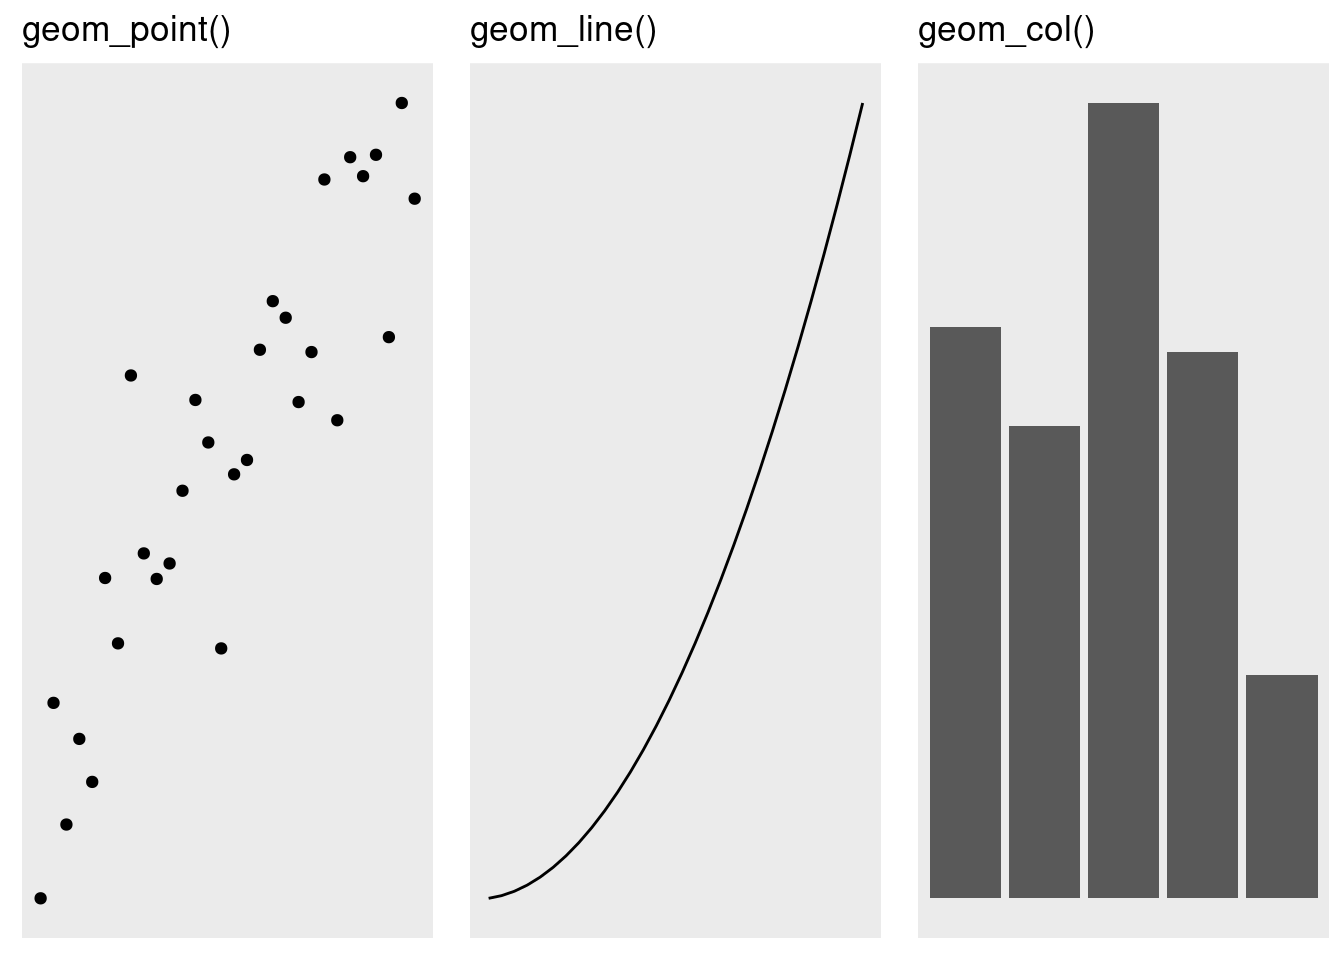
\includegraphics{img/geom.png}

\hypertarget{introducciuxf3n-a-la-visualizaciuxf3n-de-datos}{%
\subsection{Introducción a la visualización de datos}\label{introducciuxf3n-a-la-visualizaciuxf3n-de-datos}}

\begin{quote}
\textbf{Una imagen vale mas que mil palabras}.
\end{quote}

La visualización de datos es la técnica más rápida y poderosa para comprender información nueva y existente. Durante una fase de exploración inicial, los científicos de datos intentan revelar las características subyacentes de un conjunto de datos, como diferentes distribuciones, correlaciones u otros patrones visibles. Este proceso también se denomina \emph{análisis exploratorio de datos} (EDA) y marca el punto de partida de cada proyecto de ciencia de datos.

Los gráficos producidos durante la EDA muestran al científico de datos las direcciones del viaje por delante. Los patrones revelados pueden inspirar hipótesis sobre los procesos subyacentes, las características del conjunto de datos que se extraerán o las técnicas de modelado que se probarán. Por último, pero no menos importante, las visualizaciones descubren valores atípicos y errores de datos de los que el científico de datos debe ocuparse.

El papel más importante de la visualización de datos es la comunicación de los hallazgos de la ciencia de datos a colegas y clientes a través de presentaciones, informes o paneles. El esfuerzo utilizado para la EDA y las visualizaciones es un tiempo bien invertido, ya que los resultados se pueden utilizar directamente para comunicar los hallazgos.

\hypertarget{tipos-de-gruxe1ficas-disponibles}{%
\subsection{Tipos de gráficas disponibles}\label{tipos-de-gruxe1ficas-disponibles}}

Hay muchos tipos de gráficos disponibles que ayudan a comprender las diferentes características y relaciones en el conjunto de datos.

Durante la fase de análisis de datos exploratorios, normalmente queremos detectar los patrones más obvios observando cada variable de forma aislada o detectando relaciones de variables con otras. El tipo de gráfico utilizado también está determinado por el tipo de datos de las variables de entrada, como numéricas o categóricas.

\hypertarget{gruxe1fico-de-dispersiuxf3n}{%
\subsubsection{Gráfico de dispersión}\label{gruxe1fico-de-dispersiuxf3n}}

Los gráficos de dispersión se utilizan para visualizar la relación entre dos variables numéricas. La posición de cada punto representa el valor de las variables en los ejes \emph{x} e \emph{y}.

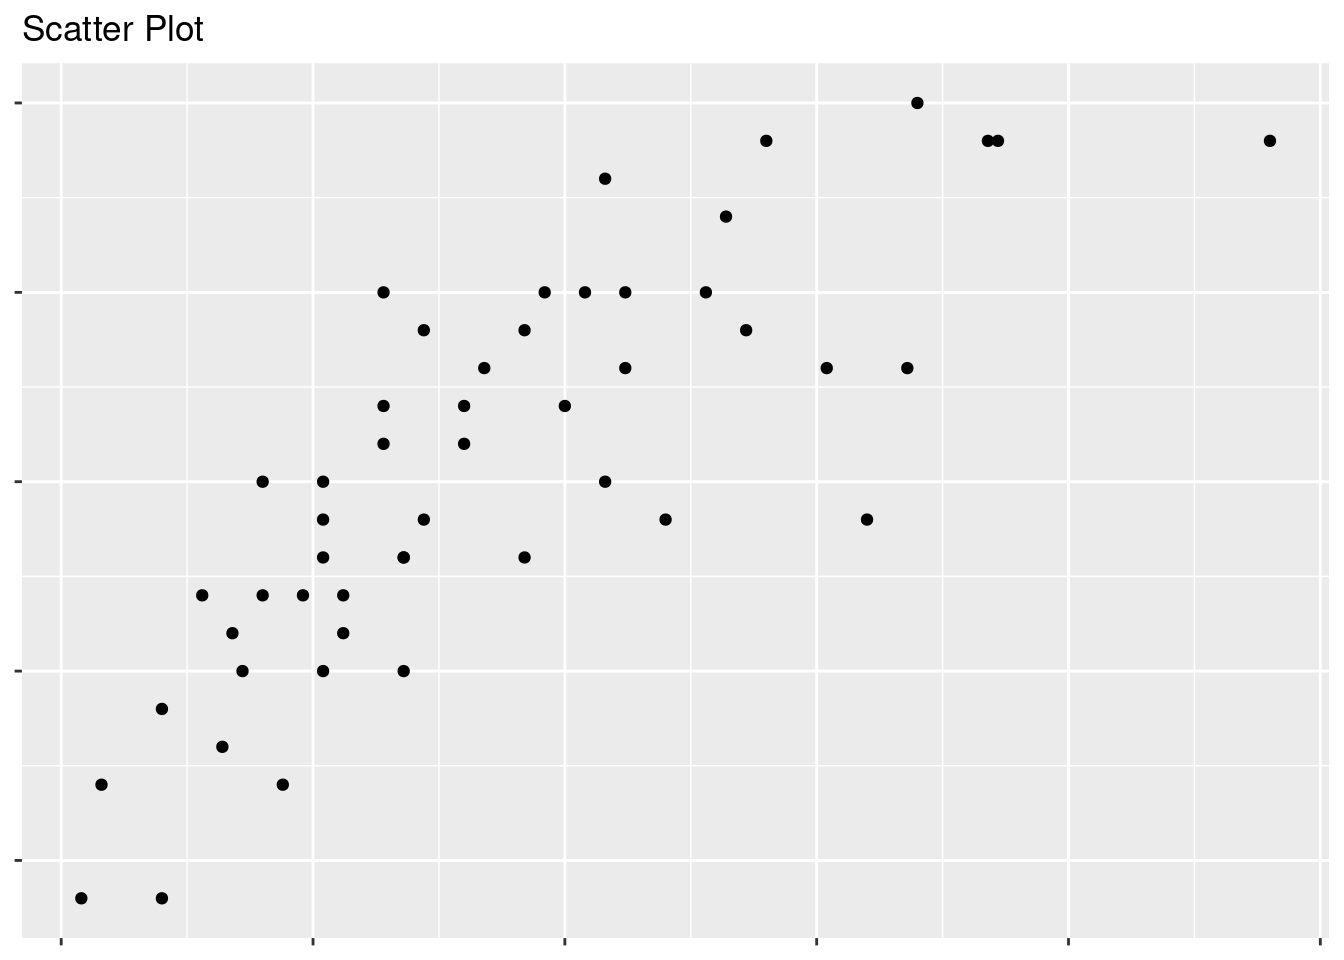
\includegraphics{img/scat.png}

\hypertarget{gruxe1ficos-lineales}{%
\subsubsection{Gráficos lineales}\label{gruxe1ficos-lineales}}

Los gráficos de líneas se utilizan para visualizar la trayectoria de una variable numérica contra otra que están conectadas a través de líneas. Son muy adecuados si los valores solo cambian \textbf{continuamente}, como la temperatura con el tiempo.

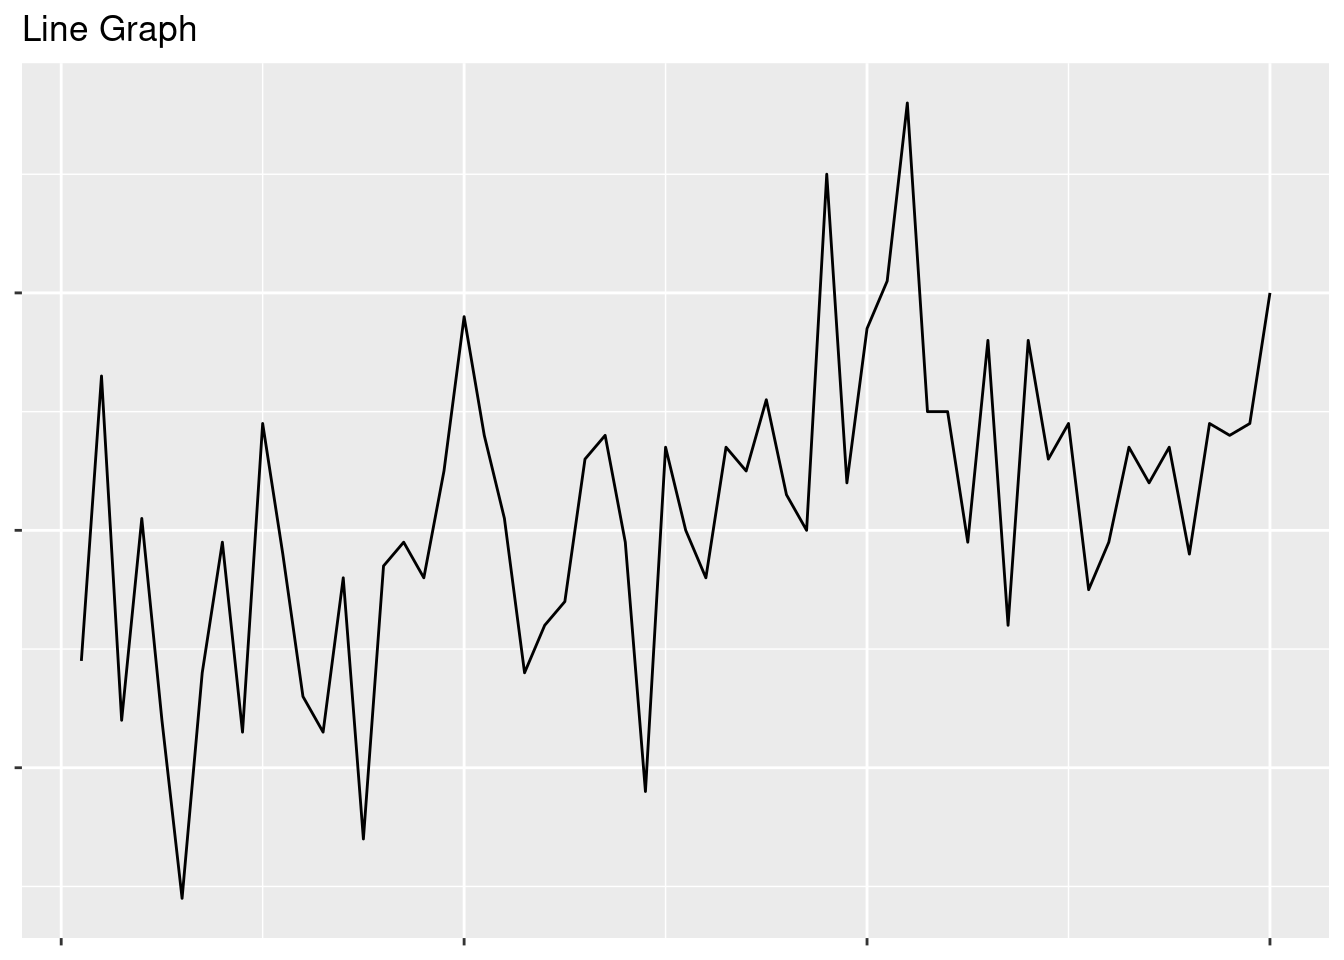
\includegraphics{img/unna.png}

\hypertarget{gruxe1ficos-de-barras-e-histogramas}{%
\subsubsection{Gráficos de barras e histogramas}\label{gruxe1ficos-de-barras-e-histogramas}}

Los gráficos de barras visualizan valores \texttt{numéricos} agrupados por categorías. Cada categoría está representada por una barra con una altura definida por cada valor \texttt{numérico}. Los histogramas son gráficos de barras específicos para resumir el número de apariciones de valores numéricos en un conjunto de rangos de valores (o bins). Suelen utilizarse para determinar la \emph{distribución} de valores numéricos.

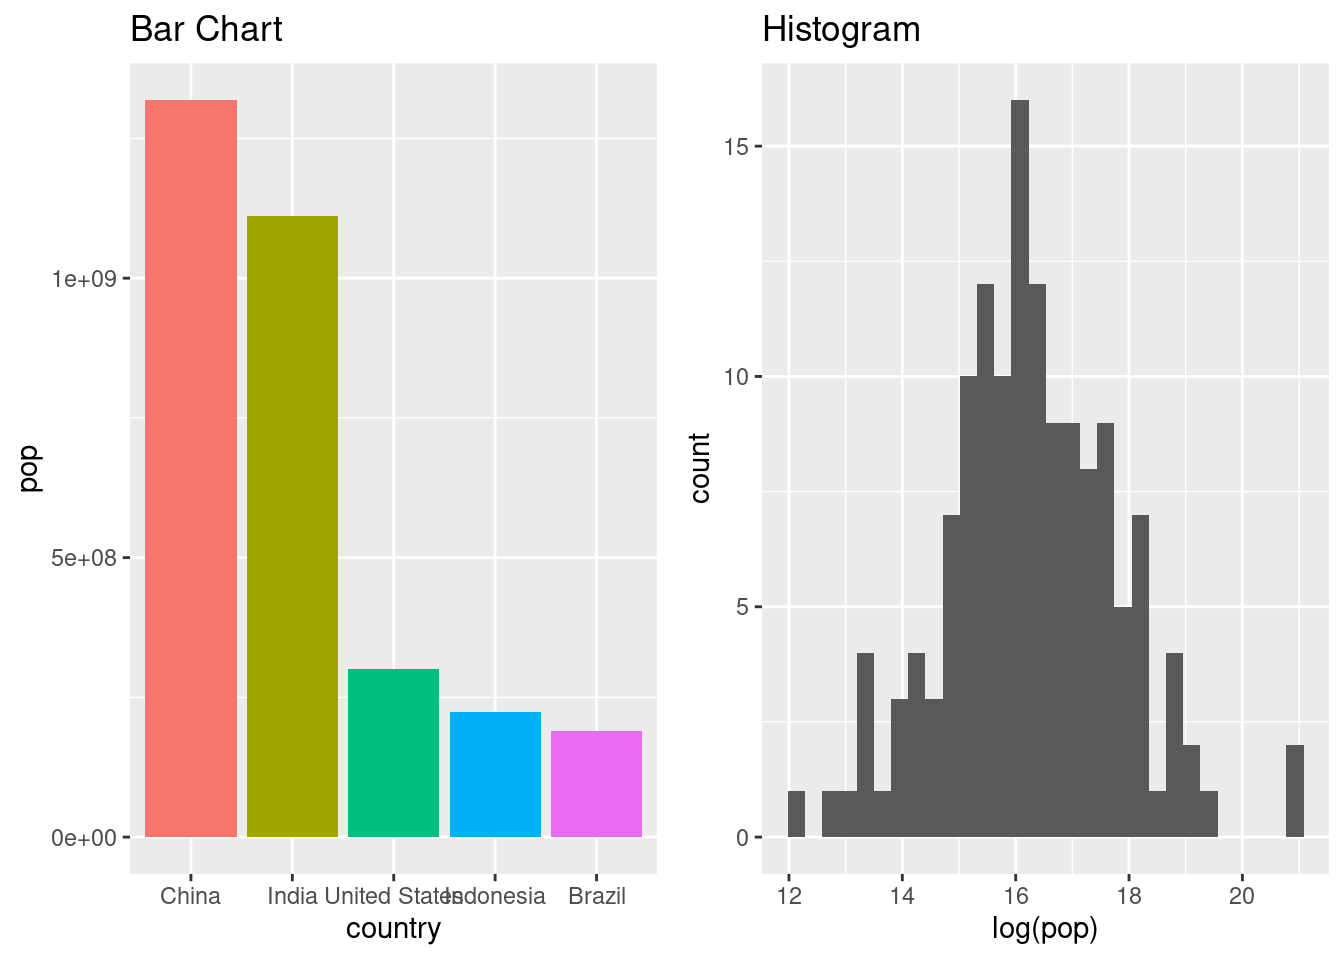
\includegraphics{img/hist.png}

\hypertarget{otros}{%
\subsubsection{Otros}\label{otros}}

Otros tipos de gráficos de uso frecuente en la ciencia de datos incluyen:

\begin{itemize}
\tightlist
\item
  \textbf{Diagramas de caja}: Muestra información de distribución de valores numéricos agrupados en categorías como cajas. Genial para comparar rápidamente múltiples distribuciones.
\item
  \textbf{Gráficos de violín}: igual que los gráficos de caja, pero muestran distribuciones como \emph{violines}.
\item
  \textbf{Mapas de calor}: muestran las interacciones de las variables, generalmente correlaciones, como imágenes rasterizadas que resaltan áreas de alta interacción.
\item
  \textbf{Gráficos de red}: muestra conexiones entre nodos
\end{itemize}

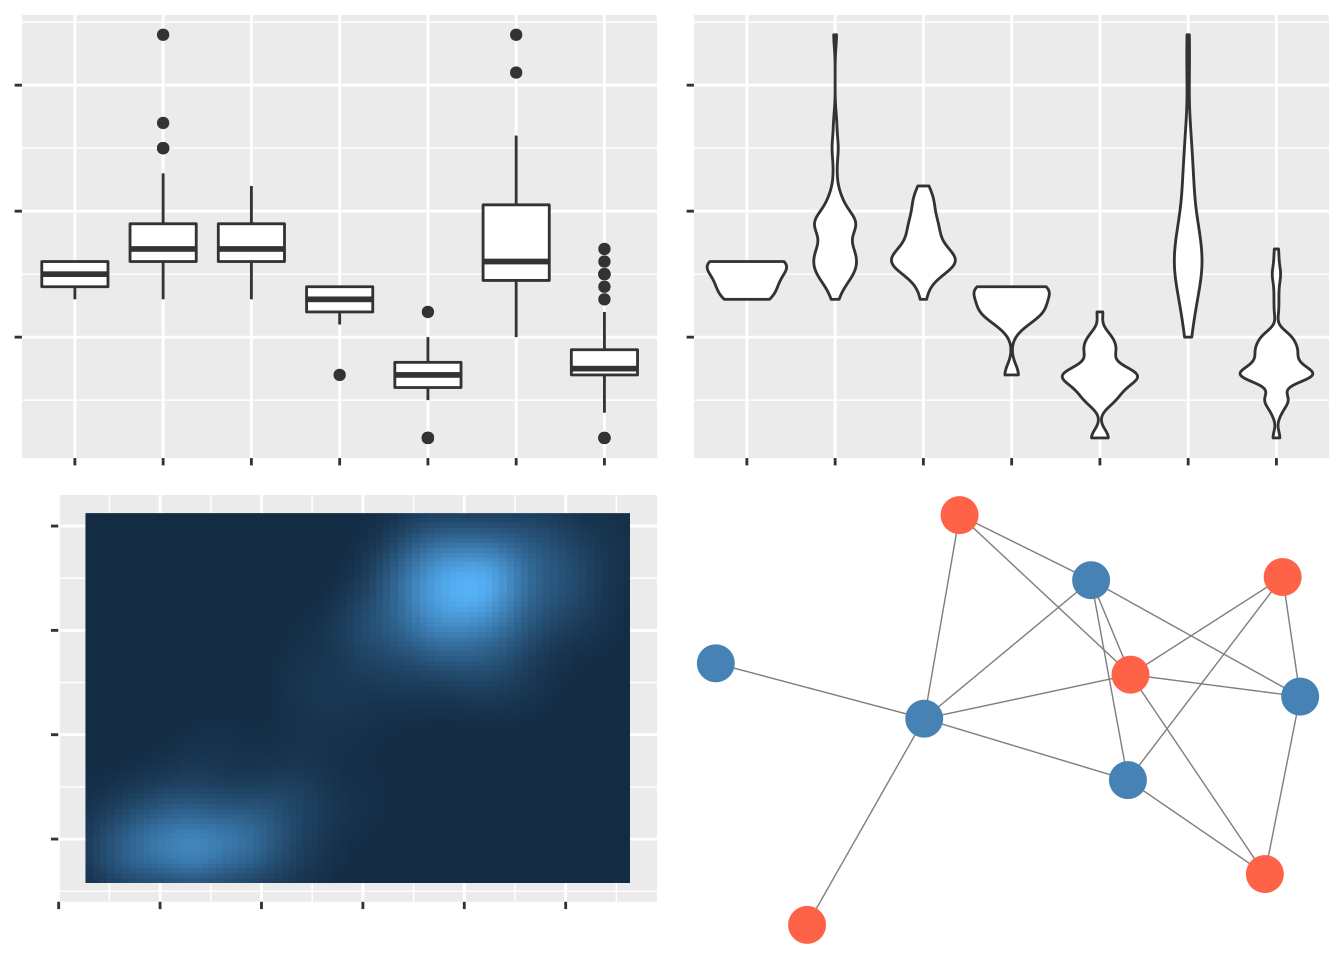
\includegraphics{img/otr.png}

\hypertarget{presentamos-ggplot2}{%
\subsection{Presentamos: ggplot2}\label{presentamos-ggplot2}}

Debido a la importancia de la visualización para la ciencia de datos y las estadísticas, R ofrece un amplio conjunto de herramientas y paquetes. El lenguaje R básico ya proporciona un rico conjunto de funciones de trazado y tipos de trazado. Estas funciones de trazado requieren que los usuarios especifiquen cómo trazar cada elemento en el lienzo paso a paso. Por el contrario, el paquete \textbf{ggplot2} permite la especificación de trazados a través de un conjunto de \emph{capas} de trazado. Esto requiere que el paquete averigüe los pasos necesarios para producir el gráfico.

A través del conjunto predefinido de capas geométricas, facetas y temas, \textbf{ggplot2} permite a los usuarios crear hermosos gráficos en muy poco tiempo. \textbf{ggplot2} es también la biblioteca de trazado más adoptada en la comunidad R.

\hypertarget{crea-un-diagrama-de-dispersiuxf3n-con-ggplot}{%
\section{Crea un diagrama de dispersión con ggplot}\label{crea-un-diagrama-de-dispersiuxf3n-con-ggplot}}

Realice sus primeros pasos con el paquete \textbf{ggplot2} para crear un diagrama de dispersión. Utilice la gramática de los gráficos para asignar los atributos del conjunto de datos a su gráfico y conectar diferentes capas con el operador \texttt{+}.

\begin{itemize}
\tightlist
\item
  Defina un conjunto de datos para la gráfica usando la función \texttt{ggplot()}
\item
  Especifique una capa geométrica usando la función \texttt{geom\_point()}
\item
  Asigne los atributos del conjunto de datos a las propiedades de trazado usando el parámetro de \texttt{mapping}
\item
  Conectar diferentes objetos \texttt{ggplot} usando el operador \texttt{+}
\end{itemize}

\begin{verbatim}
library(ggplot2)
ggplot(___) + 
  geom_point(
    mapping = aes(x = ___, y = ___)
  )
\end{verbatim}

\hypertarget{introducciuxf3n-a-los-gruxe1ficos-de-dispersiuxf3n}{%
\subsection{Introducción a los gráficos de dispersión}\label{introducciuxf3n-a-los-gruxe1ficos-de-dispersiuxf3n}}

Los diagramas de dispersión utilizan puntos para visualizar la relación entre dos variables numéricas. La posición de cada punto representa el valor de las variables en los ejes X e Y. Veamos un ejemplo de un diagrama de dispersión para comprender la relación entre la \emph{speed} y la \emph{distancia de frenado} de los automóviles:

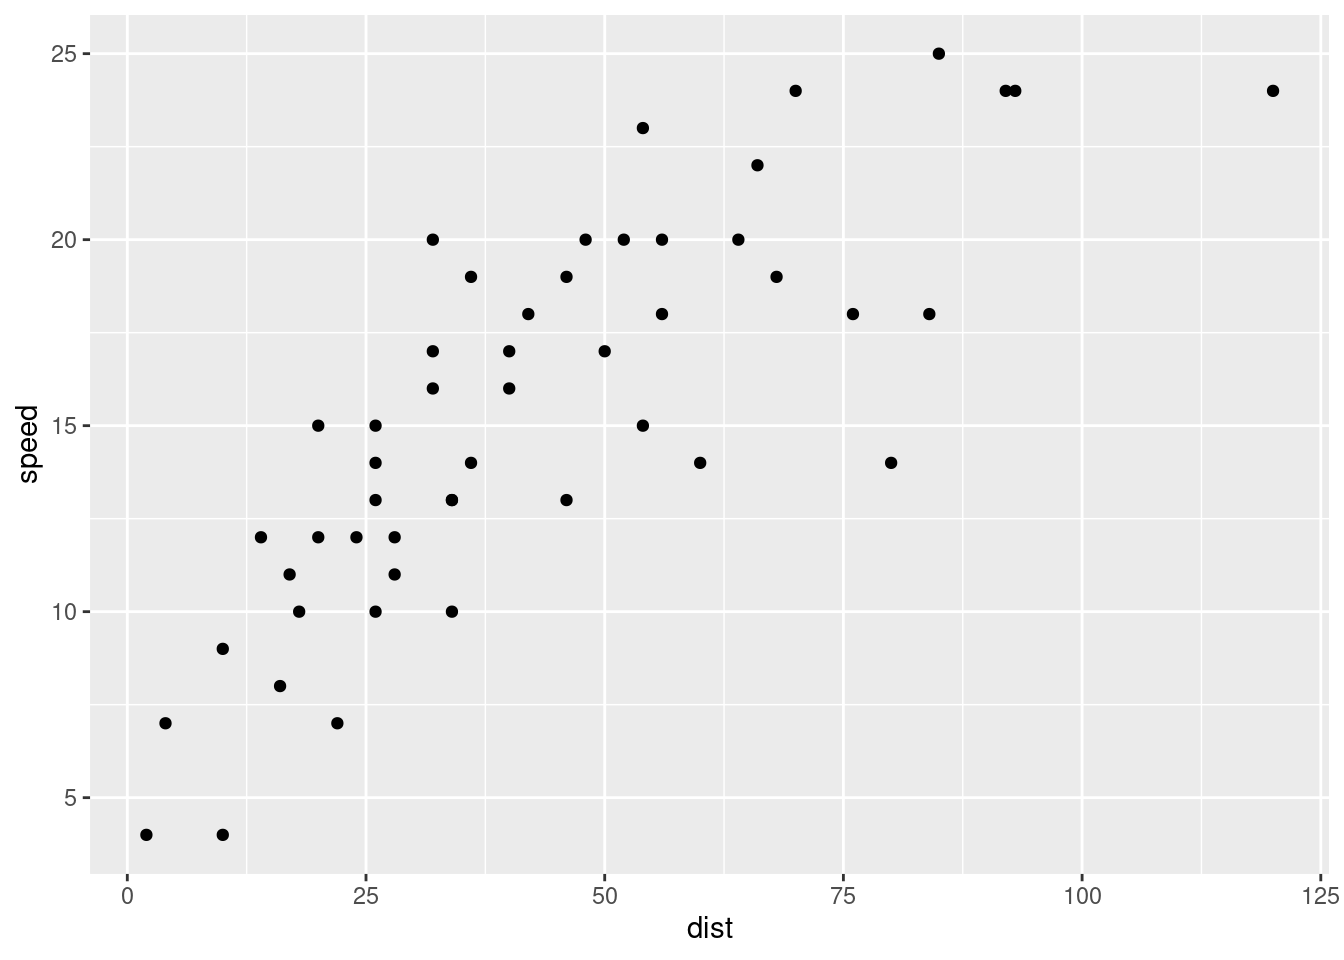
\includegraphics{img/scat1.png}

Cada punto representa un automóvil. Cada automóvil comienza a frenar a una velocidad dada en el eje-y y recorre la distancia que se muestra en el eje-x hasta detenerse por completo. Si echamos un vistazo a todos los puntos de la trama, podemos ver claramente que los coches más rápidos necesitan más distancia para detenerse por completo.

\hypertarget{especificar-un-conjunto-de-datos}{%
\subsection{Especificar un conjunto de datos}\label{especificar-un-conjunto-de-datos}}

Para crear gráficos con \textbf{ggplot2}, primero debe cargar el paquete usando la \texttt{library(ggplot2)}.

Una vez que se haya cargado el paquete, especifique el conjunto de datos que se utilizará como argumento de la función \texttt{ggplot()}. Por ejemplo, para especificar una gráfica usando el conjunto de datos de \texttt{cars}, puede usar:

\begin{Shaded}
\begin{Highlighting}[]
\FunctionTok{library}\NormalTok{(ggplot2)}
\FunctionTok{library}\NormalTok{(gapminder)}
\FunctionTok{ggplot}\NormalTok{(cars)}
\end{Highlighting}
\end{Shaded}


\includegraphics{BookR_files/figure-latex/unnamed-chunk-118-1.pdf}

Tenga en cuenta que este comando no traza nada más que un lienzo gris todavía. Simplemente define el conjunto de datos para el gráfico y crea una base vacía sobre la cual podemos agregar capas adicionales.

\hypertarget{especificando-una-capa-geomuxe9trica}{%
\subsection{Especificando una capa geométrica}\label{especificando-una-capa-geomuxe9trica}}

Podemos usar las capas geométricas de \textbf{ggplot} (o \emph{geoms}) para definir cómo queremos visualizar nuestro conjunto de datos. Las \emph{geoms} utilizan objetos geométricos para visualizar las variables de un conjunto de datos. Los objetos pueden tener múltiples formas como puntos, líneas y barras y se especifican mediante las funciones correspondientes \texttt{geom\_point()}, \texttt{geom\_line()} y \texttt{geom\_col()}:

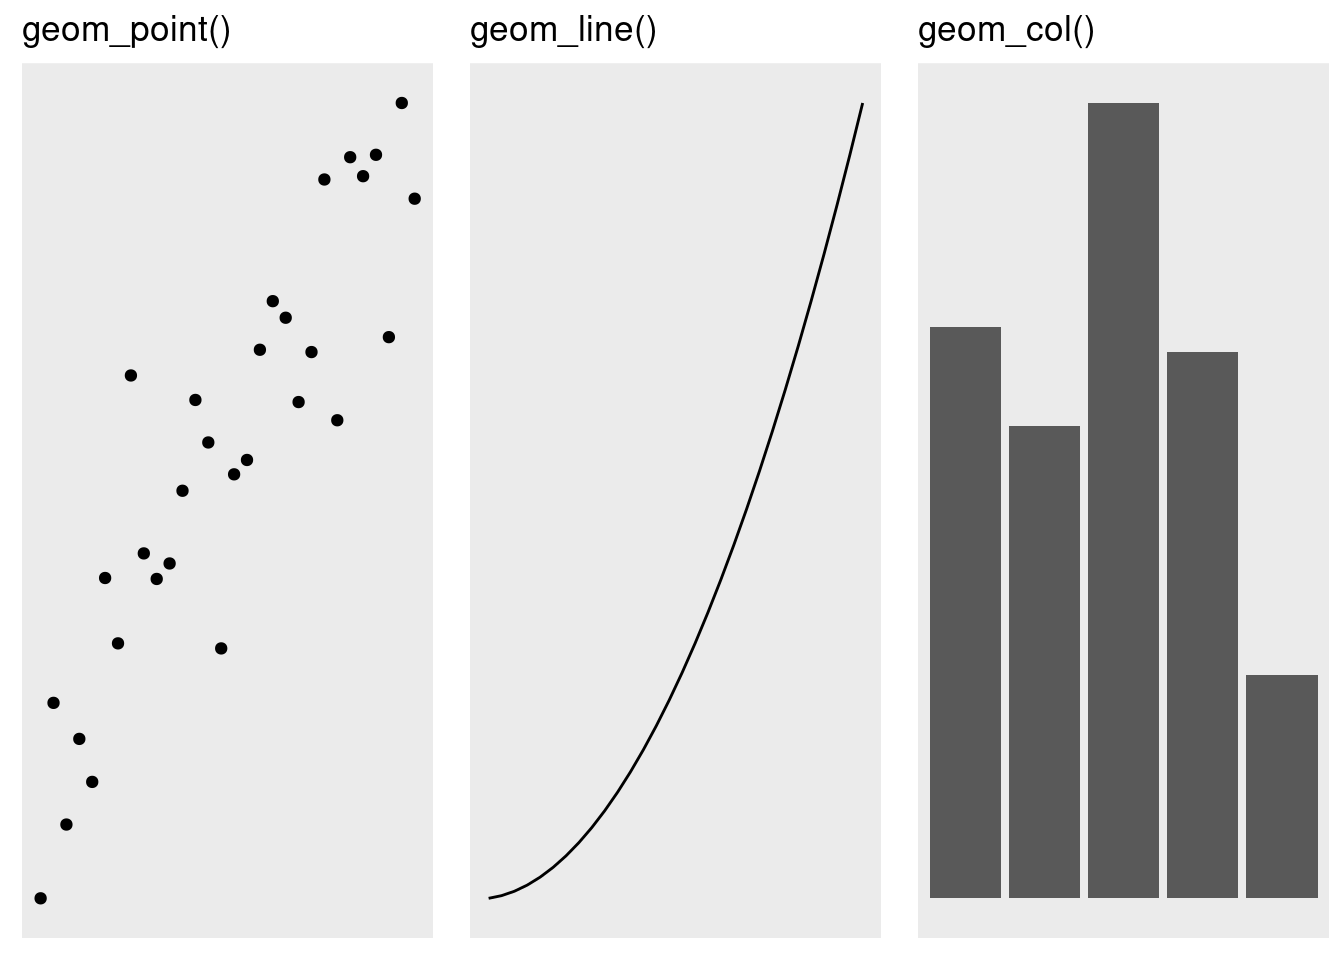
\includegraphics{img/geom.png}

\hypertarget{creando-mapeos-estuxe9ticos}{%
\subsection{Creando mapeos estéticos}\label{creando-mapeos-estuxe9ticos}}

\textbf{ggplot2} utiliza el concepto de \emph{estética}, que \emph{asigna} los atributos del conjunto de datos a las características visuales de la gráfica. Cada capa geométrica requiere un conjunto diferente de \emph{asignaciones estéticas}, p.~Ej. la función \texttt{geom\_point()} usa la estética \texttt{x} e \texttt{y} para determinar las coordenadas de los ejes \texttt{x} e \texttt{y} de los puntos a graficar. La estética se asigna dentro de la función \texttt{aes()} para construir las asignaciones finales.

Para especificar una capa de puntos que traza la velocidad variable en el eje-x y la distancia \texttt{dist} en el eje-y, podemos escribir:

\begin{Shaded}
\begin{Highlighting}[]
\FunctionTok{geom\_point}\NormalTok{(}
  \AttributeTok{mapping =} \FunctionTok{aes}\NormalTok{(}\AttributeTok{x=}\NormalTok{speed, }\AttributeTok{y=}\NormalTok{dist)}
\NormalTok{)}
\end{Highlighting}
\end{Shaded}

La expresión anterior construye una capa geométrica. Sin embargo, esta capa actualmente no está vinculada a un conjunto de datos y no produce una gráfica. Para \textbf{vincular} la capa con un objeto \texttt{ggplot} que especifica el conjunto de datos de \texttt{cars}, necesitamos conectar el objeto \texttt{ggplot(cars)} con la capa \texttt{geom\_point()} usando el operador \texttt{+}:

\begin{Shaded}
\begin{Highlighting}[]
\FunctionTok{ggplot}\NormalTok{(cars) }\SpecialCharTok{+} 
  \FunctionTok{geom\_point}\NormalTok{(}
    \AttributeTok{mapping =} \FunctionTok{aes}\NormalTok{(}\AttributeTok{x=}\NormalTok{speed, }\AttributeTok{y=}\NormalTok{dist)}
\NormalTok{  )}
\end{Highlighting}
\end{Shaded}

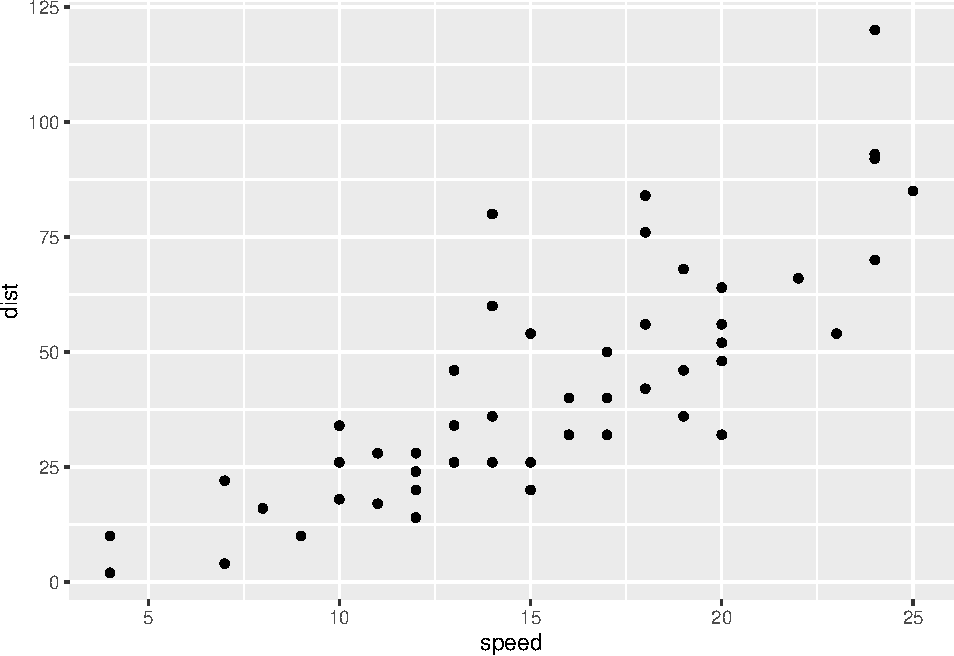
\includegraphics{BookR_files/figure-latex/unnamed-chunk-120-1.pdf}

A través del enlace, \texttt{ggplot()} sabe que las variables de \texttt{speed} y \texttt{dist} asignadas se toman del conjunto de datos de \texttt{cars}. \texttt{geom\_point()} instruye a ggplot para trazar las variables mapeadas como puntos.

Los pasos necesarios para crear un diagrama de dispersión con \texttt{ggplot} se pueden resumir de la siguiente manera:

\begin{enumerate}
\def\labelenumi{\arabic{enumi}.}
\tightlist
\item
  Cargue el paquete \textbf{ggplot2} usando \texttt{library(ggplot2)}.
\item
  Especifique el conjunto de datos que se graficará usando \texttt{ggplot()}.
\item
  Utilice el operador \texttt{+} para agregar capas al gráfico.
\item
  Agregue una capa geométrica para definir las formas que se graficaran. En caso de gráficos de dispersión, use \texttt{geom\_point()}.
\item
  Asigne variables del conjunto de datos a propiedades de trazado a través del parámetro de \texttt{mapping} en la capa geométrica.
\end{enumerate}

\hypertarget{especificar-estuxe9tica-adicional-para-puntos}{%
\section{Especificar estética adicional para puntos}\label{especificar-estuxe9tica-adicional-para-puntos}}

\textbf{ggplot2} implementa la gramática de gráficos para mapear atributos de un conjunto de datos para trazar características a través de la estética. Este marco se puede utilizar para ajustar el \texttt{tamaño\ de\ punto}, el \texttt{color} y la transparencia \texttt{alpha} de los puntos en un diagrama de dispersión.

\begin{itemize}
\tightlist
\item
  Agregue dimensiones de trazado adicionales a través de la estética
\item
  Ajuste el tamaño del punto de un gráfico de dispersión usando el parámetro \texttt{size}
\item
  Cambiar el color del punto de un diagrama de dispersión usando el parámetro \texttt{color}
\item
  Establecer un parámetro \texttt{alpha} para cambiar la transparencia de todos los puntos
\item
  Diferenciar entre mapeos estéticos y parámetros constantes
\end{itemize}

\begin{verbatim}
ggplot(___) + 
  geom_point(
    mapping = aes(x = ___, y = ___, 
                  color = ___, 
                  size  = ___),
    alpha  = ___
  )
\end{verbatim}

\hypertarget{auxf1adiendo-muxe1s-estuxe9tica-a-la-trama}{%
\subsection{Añadiendo más estética a la trama}\label{auxf1adiendo-muxe1s-estuxe9tica-a-la-trama}}

En su forma más básica, los diagramas de dispersión solo pueden visualizar conjuntos de datos en dos dimensiones a través de la estética \texttt{x} e \texttt{y} de la capa \texttt{geom\_point()}. Sin embargo, la mayoría de los conjuntos de datos tienen más de dos variables y, por lo tanto, pueden requerir dimensiones de trazado adicionales. \texttt{ggplot()} hace que sea muy fácil mapear variables adicionales a diferentes estéticas de trazado como \texttt{size}, transparencia \texttt{alpha} y \texttt{color}.

Consideremos el conjunto de datos \texttt{gapminder\_2007} que contiene las variables PIB per cápita \texttt{gdpPercap} y esperanza de vida \texttt{lifeExp} para 142 países en el año 2007:

\begin{Shaded}
\begin{Highlighting}[]
\FunctionTok{library}\NormalTok{(tidyverse)}
\FunctionTok{library}\NormalTok{(gapminder)}
\DocumentationTok{\#\# select data}
\NormalTok{gapminder\_2007 }\OtherTok{\textless{}{-}}\NormalTok{ gapminder}\SpecialCharTok{\%\textgreater{}\%}
  \FunctionTok{filter}\NormalTok{(year }\SpecialCharTok{==} \DecValTok{2007}\NormalTok{)}
\end{Highlighting}
\end{Shaded}

\begin{Shaded}
\begin{Highlighting}[]
\FunctionTok{ggplot}\NormalTok{(gapminder\_2007) }\SpecialCharTok{+} 
  \FunctionTok{geom\_point}\NormalTok{(}\FunctionTok{aes}\NormalTok{(}\AttributeTok{x =}\NormalTok{ gdpPercap, }\AttributeTok{y =}\NormalTok{ lifeExp))}
\end{Highlighting}
\end{Shaded}

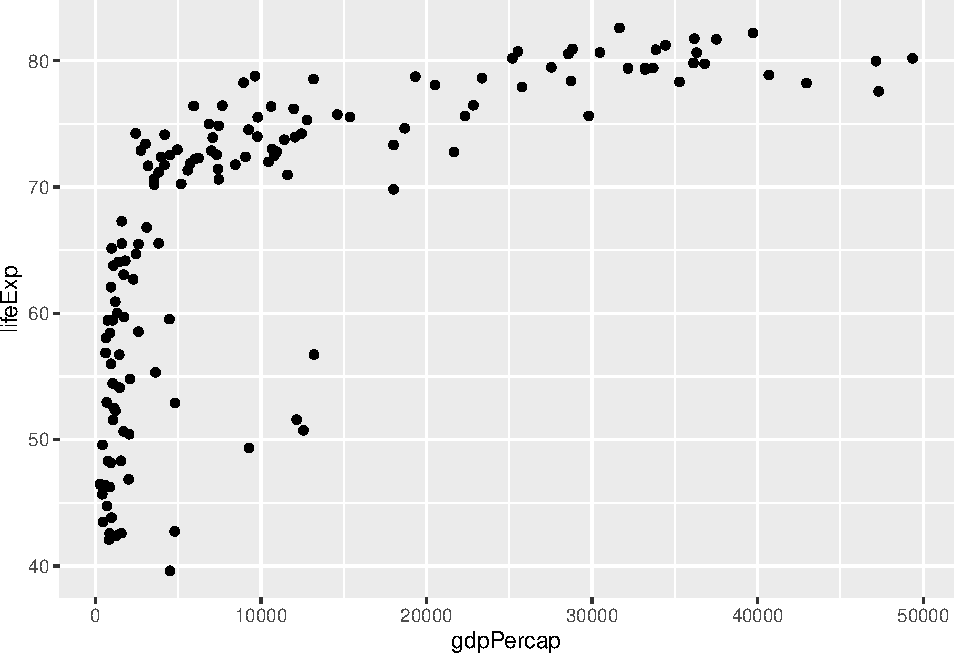
\includegraphics{BookR_files/figure-latex/unnamed-chunk-122-1.pdf}

Al mapear la variable \texttt{continent} a través de la estética del \texttt{color} del punto y la población \texttt{pop} (en millones) a través del tamaño del punto \texttt{size}, obtenemos una gráfica mucho más rica que incluye 4 variables diferentes del conjunto de datos:

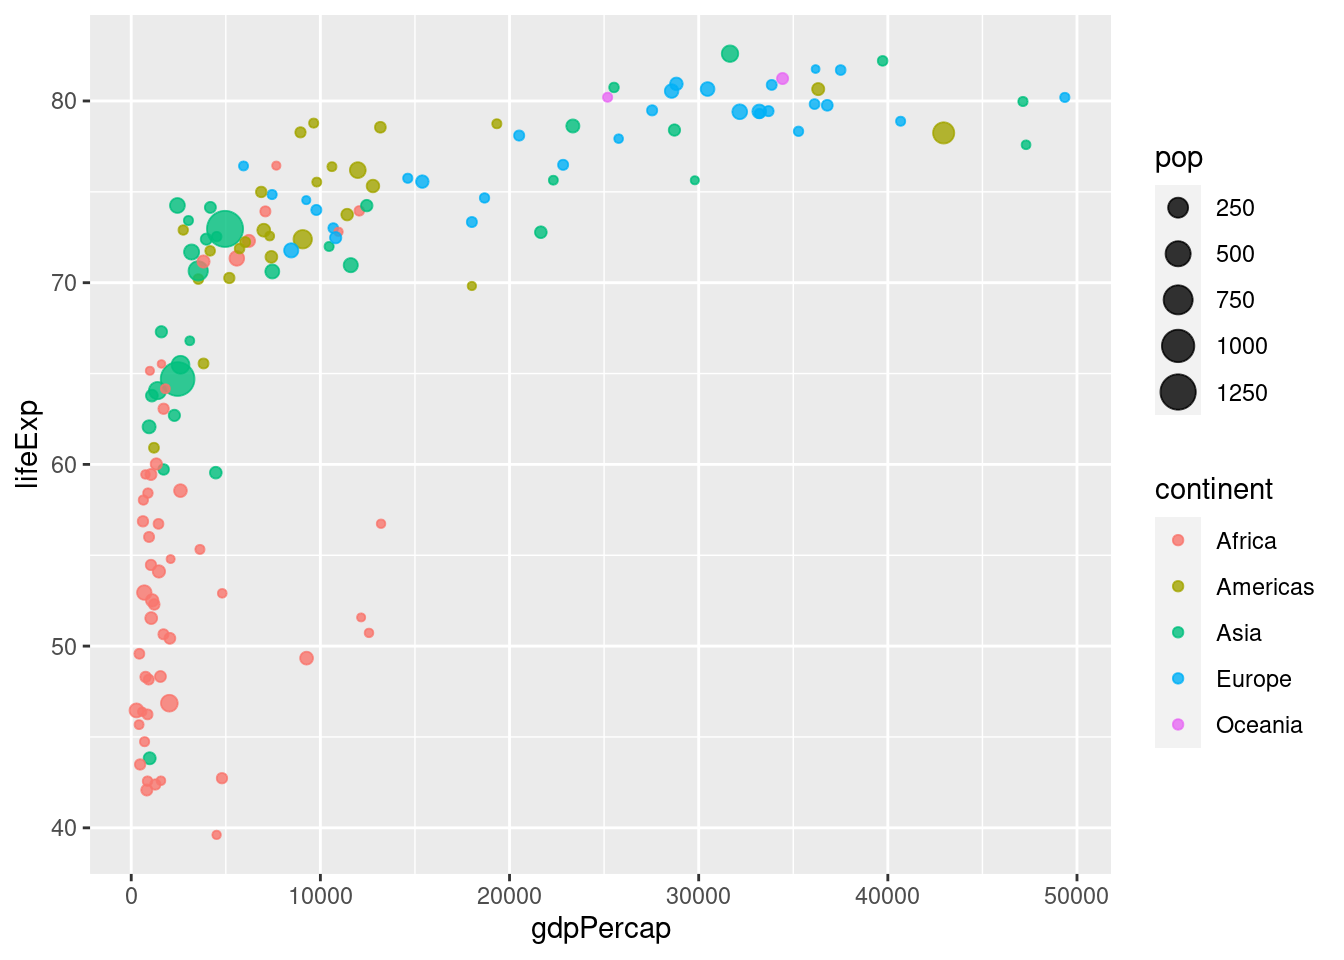
\includegraphics{img/un4.png}

\hypertarget{ajuste-del-color-del-punto}{%
\subsection{Ajuste del color del punto}\label{ajuste-del-color-del-punto}}

Normalmente, el color del punto se utiliza para introducir una nueva dimensión en un diagrama de dispersión. En ggplot usamos la estética del \texttt{color} para especificar el mapeo de una variable al color de los puntos.

Para el conjunto de datos \texttt{gapminder\_2007} podemos trazar el PIB per cápita \texttt{gdpPercap} frente a la esperanza de vida \texttt{lifeExp} de la siguiente manera:

\begin{Shaded}
\begin{Highlighting}[]
\FunctionTok{ggplot}\NormalTok{(gapminder\_2007) }\SpecialCharTok{+} 
  \FunctionTok{geom\_point}\NormalTok{(}\FunctionTok{aes}\NormalTok{(}\AttributeTok{x =}\NormalTok{ gdpPercap, }\AttributeTok{y =}\NormalTok{ lifeExp))}
\end{Highlighting}
\end{Shaded}

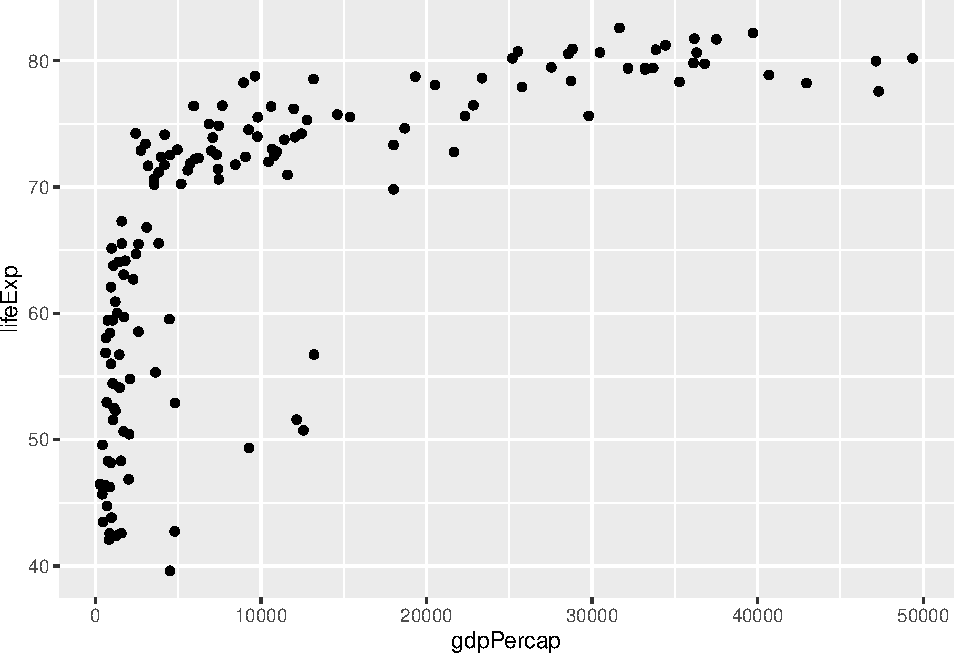
\includegraphics{BookR_files/figure-latex/unnamed-chunk-123-1.pdf}

Para colorear cada punto en función del \texttt{continent} de cada país podemos utilizar:

\begin{Shaded}
\begin{Highlighting}[]
\FunctionTok{ggplot}\NormalTok{(gapminder\_2007) }\SpecialCharTok{+} 
  \FunctionTok{geom\_point}\NormalTok{(}\FunctionTok{aes}\NormalTok{(}\AttributeTok{x =}\NormalTok{ gdpPercap, }\AttributeTok{y =}\NormalTok{ lifeExp,}
                 \AttributeTok{color =}\NormalTok{ continent))}
\end{Highlighting}
\end{Shaded}

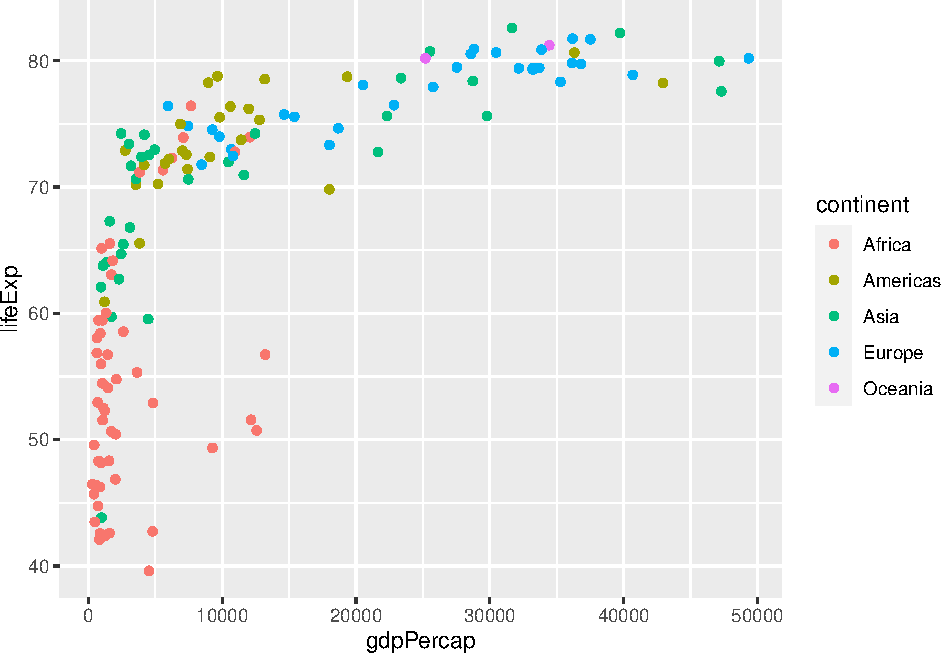
\includegraphics{BookR_files/figure-latex/unnamed-chunk-124-1.pdf}

Vemos que en la trama resultante cada punto está coloreado de manera diferente según el \texttt{continent} de cada país. \texttt{ggplot} usa el esquema de coloración basado en el tipo de datos categóricos de la variable \texttt{continent}.

Por el contrario, veamos cómo se ve el gráfico si coloreamos los puntos por el \texttt{pop} de población de la variable \texttt{numeric}:

\begin{Shaded}
\begin{Highlighting}[]
\FunctionTok{ggplot}\NormalTok{(gapminder\_2007) }\SpecialCharTok{+} 
  \FunctionTok{geom\_point}\NormalTok{(}\FunctionTok{aes}\NormalTok{(}\AttributeTok{x =}\NormalTok{ gdpPercap, }\AttributeTok{y =}\NormalTok{ lifeExp,}
                 \AttributeTok{color =}\NormalTok{ pop))}
\end{Highlighting}
\end{Shaded}

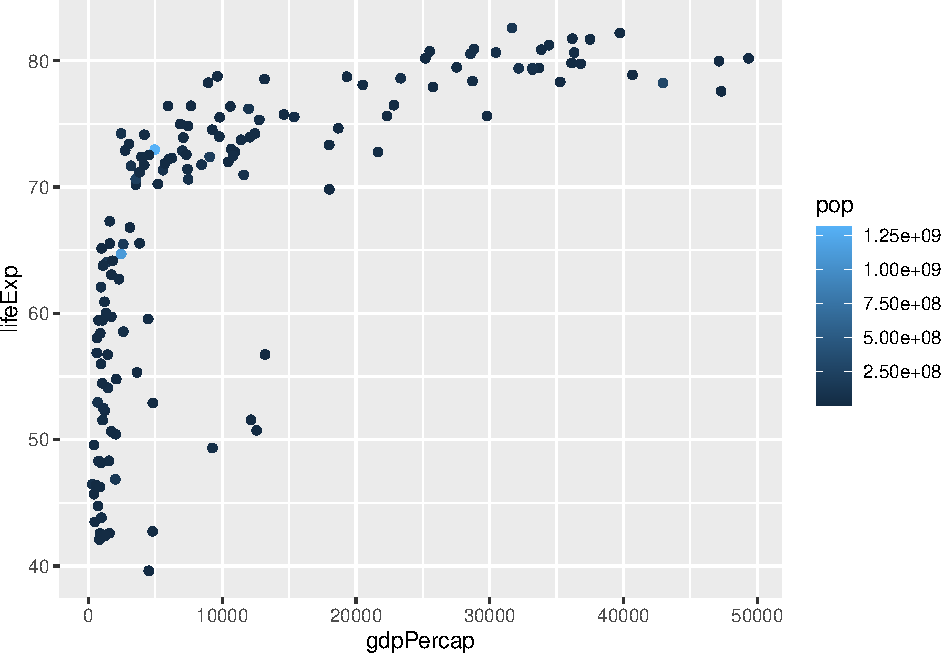
\includegraphics{BookR_files/figure-latex/unnamed-chunk-125-1.pdf}

La escala cambia inmediatamente a continua como se puede ver en la leyenda y los puntos celestes son ahora los países con mayor número de población (China e India).

\hypertarget{ajustar-el-tamauxf1o-del-punto}{%
\subsection{Ajustar el tamaño del punto}\label{ajustar-el-tamauxf1o-del-punto}}

Para el conjunto de datos de \texttt{gapminder\_2007} podemos trazar el PIB per cápita \texttt{gdpPercap} frente a la esperanza de vida de la siguiente manera:

\begin{Shaded}
\begin{Highlighting}[]
\FunctionTok{ggplot}\NormalTok{(gapminder\_2007) }\SpecialCharTok{+} 
  \FunctionTok{geom\_point}\NormalTok{(}\FunctionTok{aes}\NormalTok{(}\AttributeTok{x =}\NormalTok{ gdpPercap, }
                 \AttributeTok{y =}\NormalTok{ lifeExp))}
\end{Highlighting}
\end{Shaded}

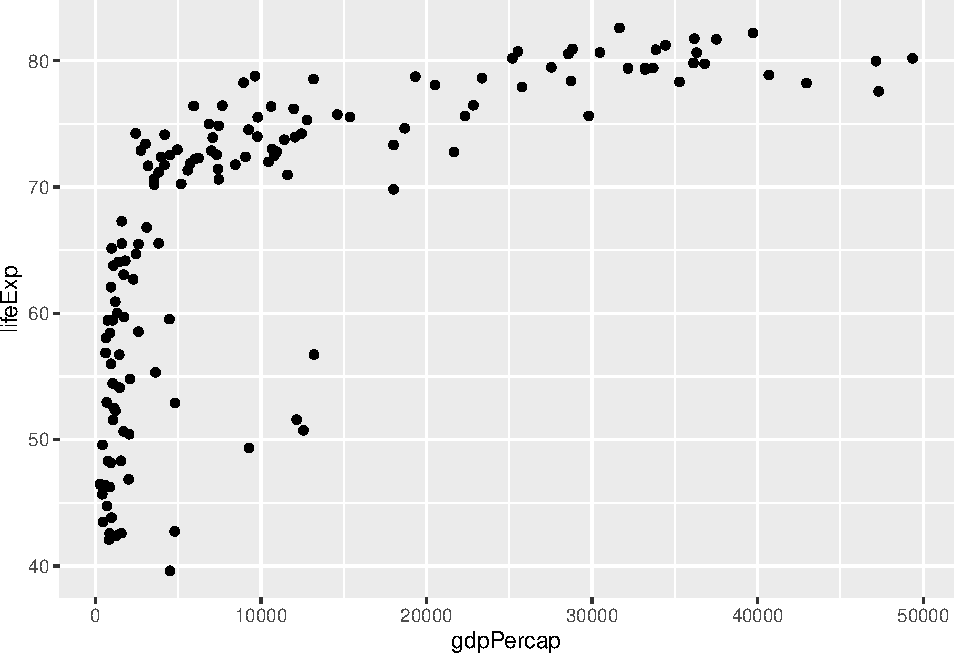
\includegraphics{BookR_files/figure-latex/unnamed-chunk-126-1.pdf}

Para ajustar el tamaño de puntos en función de la población (\texttt{pop}) de cada país, podemos usar:

\begin{Shaded}
\begin{Highlighting}[]
\FunctionTok{ggplot}\NormalTok{(gapminder\_2007) }\SpecialCharTok{+} 
  \FunctionTok{geom\_point}\NormalTok{(}\FunctionTok{aes}\NormalTok{(}\AttributeTok{x =}\NormalTok{ gdpPercap, }\AttributeTok{y =}\NormalTok{ lifeExp,}
                 \AttributeTok{size =}\NormalTok{ pop))}
\end{Highlighting}
\end{Shaded}

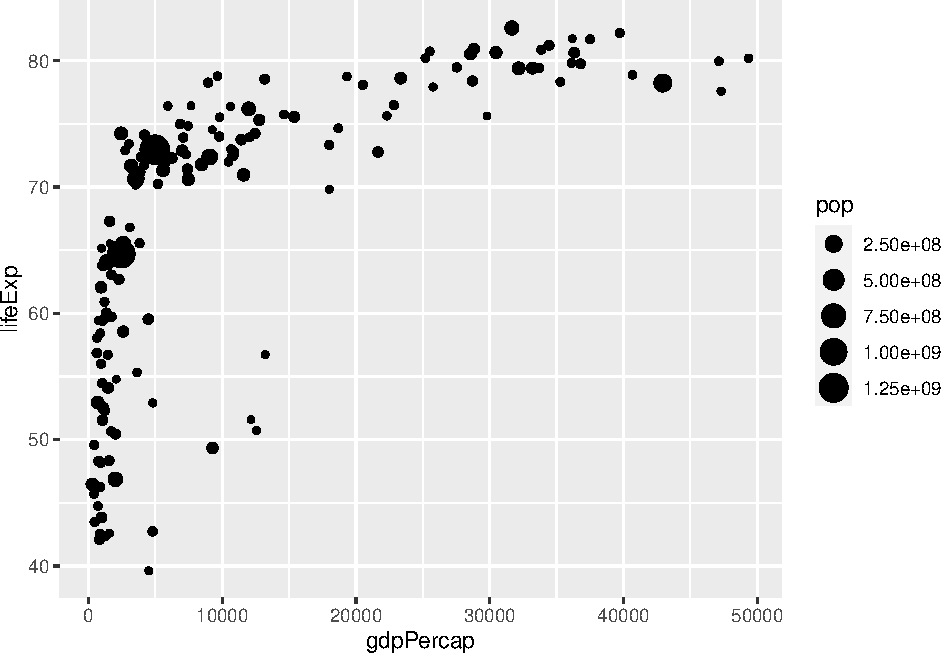
\includegraphics{BookR_files/figure-latex/unnamed-chunk-127-1.pdf}

Vemos que los tamaños de puntos en el gráfico anterior no reflejan claramente las diferencias de población en cada país. Si comparamos el tamaño en puntos que representa una población de 250 millones de personas con el que muestra 750 millones, podemos ver que sus tamaños no son proporcionales. En su lugar, los tamaños en puntos están agrupados de forma predeterminada. Para reflejar las diferencias de población reales por el tamaño de puntos, podemos usar la función \texttt{scale\_size\_area()} en su lugar. La información de escala se puede agregar como cualquier otro objeto ggplot con el operador \texttt{+}:

\begin{Shaded}
\begin{Highlighting}[]
\FunctionTok{ggplot}\NormalTok{(gapminder\_2007) }\SpecialCharTok{+} 
  \FunctionTok{geom\_point}\NormalTok{(}\FunctionTok{aes}\NormalTok{(}\AttributeTok{x =}\NormalTok{ gdpPercap, }\AttributeTok{y =}\NormalTok{ lifeExp,}
                 \AttributeTok{color =}\NormalTok{ continent,}
                 \AttributeTok{size =}\NormalTok{ pop)) }\SpecialCharTok{+} 
  \FunctionTok{scale\_size\_area}\NormalTok{(}\AttributeTok{max\_size =} \DecValTok{10}\NormalTok{)}
\end{Highlighting}
\end{Shaded}

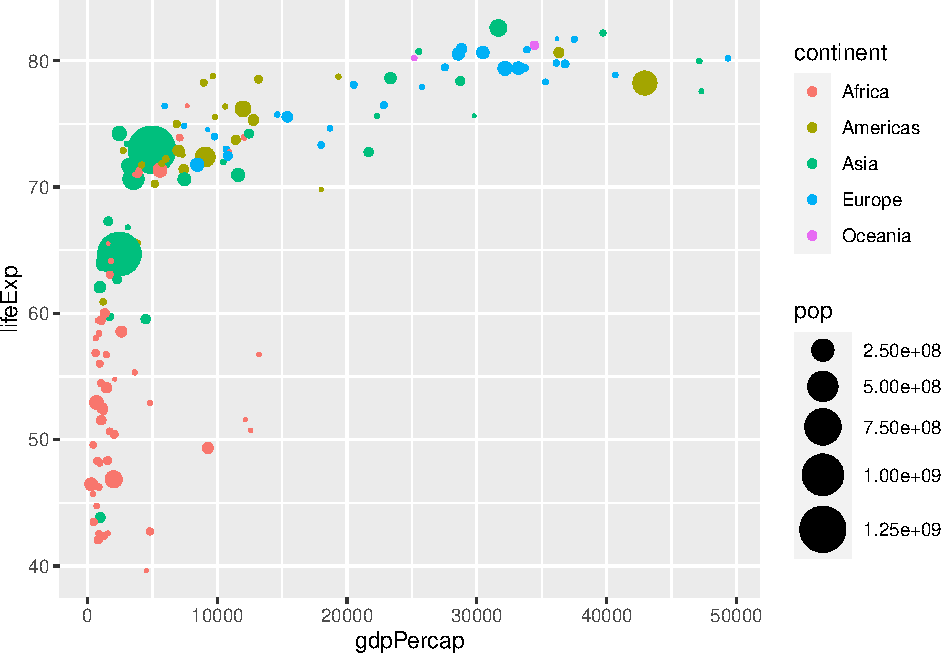
\includegraphics{BookR_files/figure-latex/unnamed-chunk-128-1.pdf}

Tenga en cuenta que hemos ajustado el tamaño del punto con \texttt{max\_size}, lo que da como resultado tamaños de punto más grandes.

\hypertarget{establecer-la-estuxe9tica-global-transparencia}{%
\subsection{Establecer la estética global: transparencia}\label{establecer-la-estuxe9tica-global-transparencia}}

Trazar muchos puntos con coordenadas X e Y similares en un gráfico puede producir nubes de puntos densas. Muchos puntos en estas nubes están sobretrazados y el número real de observaciones en un área determinada ya no es visible. Como solución, podemos establecer la transparencia de cada punto usando el parámetro ggplot \texttt{alpha}.

Dado que \textbf{no} queremos establecer la transparencia del punto \textbf{individualmente} para cada punto sino \textbf{globalmente} para todos los puntos, no establecemos el parámetro \texttt{alpha} como un mapeo estético (dentro de \texttt{aes()}) sino fuera.

Establecemos la \textbf{opacidad} de cada punto al 50\% a través del parámetro \texttt{alpha} \textbf{outside} como parámetro constante:

\begin{Shaded}
\begin{Highlighting}[]
\FunctionTok{ggplot}\NormalTok{(gapminder\_2007) }\SpecialCharTok{+} 
  \FunctionTok{geom\_point}\NormalTok{(}\FunctionTok{aes}\NormalTok{(}\AttributeTok{x =}\NormalTok{ gdpPercap, }\AttributeTok{y =}\NormalTok{ lifeExp, }\AttributeTok{size =}\NormalTok{ pop), }
             \AttributeTok{alpha =} \FloatTok{0.5}\NormalTok{)}
\end{Highlighting}
\end{Shaded}

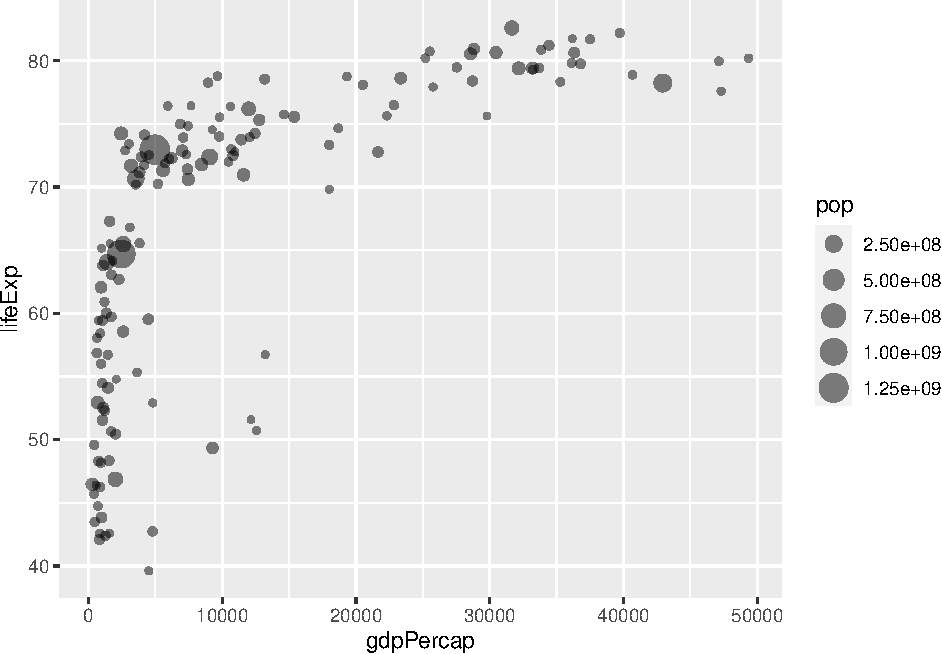
\includegraphics{BookR_files/figure-latex/unnamed-chunk-129-1.pdf}

Ahora podemos ver claramente cuántos puntos se superponen entre sí y la opacidad de cada punto se establece en \texttt{0.5}.

\hypertarget{crea-un-gruxe1fico-de-luxedneas-con-ggplot}{%
\section{Crea un gráfico de líneas con ggplot}\label{crea-un-gruxe1fico-de-luxedneas-con-ggplot}}

Use la estética \texttt{geom\_line()} para dibujar gráficos de líneas y personalizar su estilo usando el parámetro \texttt{color}. Especifique qué coordenadas usar para cada línea con el parámetro \texttt{group}.

\begin{itemize}
\tightlist
\item
  Crea tu primer gráfico de línea usando \texttt{geom\_line()}
\item
  Defina cómo se conectan las diferentes líneas mediante el parámetro \texttt{group}
\item
  Cambiar el color de línea de un gráfico de líneas usando el parámetro \texttt{color}
\end{itemize}

\begin{verbatim}
ggplot(___) + 
  geom_line(
    mapping = aes(x = ___, y = ___, 
                  group = ___, 
                  color = ___)
)
\end{verbatim}

\hypertarget{introducciuxf3n-a-los-gruxe1ficos-lineales}{%
\subsection{Introducción a los gráficos lineales}\label{introducciuxf3n-a-los-gruxe1ficos-lineales}}

Los gráficos de líneas se utilizan para visualizar la trayectoria de una variable numérica contra otra. A diferencia de los diagramas de dispersión, las coordenadas \texttt{x} e \texttt{y} no se visualizan a través de puntos, sino que están conectadas a través de líneas. Los gráficos de líneas se utilizan con mayor frecuencia si una variable cambia \emph{continuamente} contra otra variable numérica, como es el caso de la mayoría de los gráficos de series de tiempo (por ejemplo, precios, clientes, concentración de CO2, temperatura a lo largo del tiempo), funciones continuas (por ejemplo, sinusoidal (x)) u otras relaciones casi continuas (curvas de oferta/demanda del mundo real).

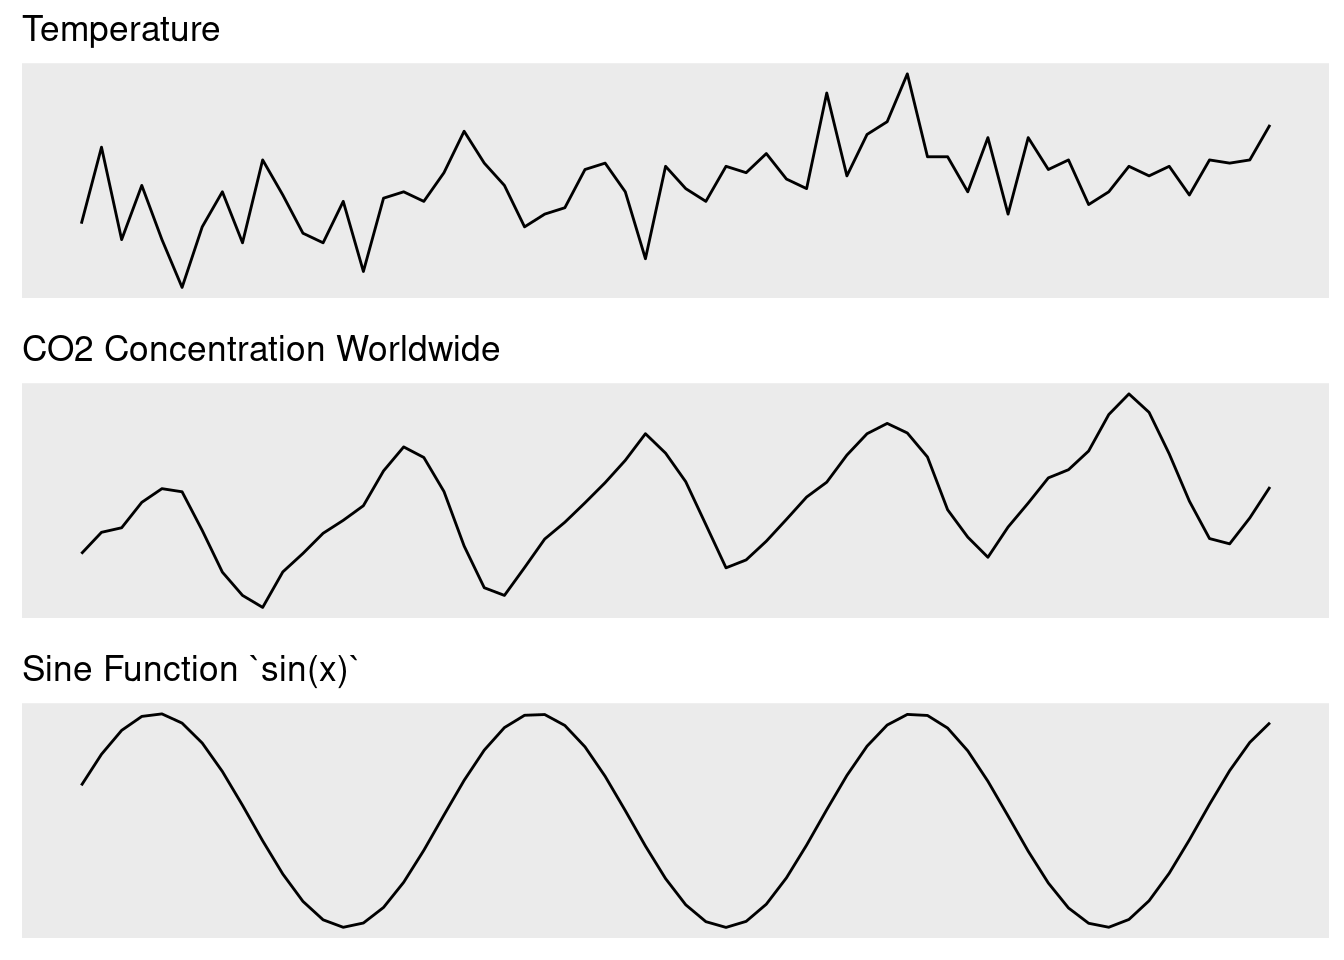
\includegraphics{img/geo1.png}

\hypertarget{crear-un-gruxe1fico-lineal-simple}{%
\subsection{Crear un gráfico lineal simple}\label{crear-un-gruxe1fico-lineal-simple}}

Japón se encuentra entre los países con mayor esperanza de vida. Utilizando el conjunto de datos \texttt{gapminder\_japan}, determinamos cómo se ha desarrollado la esperanza de vida en Japón a lo largo del tiempo. Necesitamos que:

\begin{enumerate}
\def\labelenumi{\arabic{enumi}.}
\tightlist
\item
  Especifique el conjunto de datos dentro de \texttt{ggplot()}
\item
  Definir la capa de trazado \texttt{geom\_line()}
\item
  Asigne el \texttt{year} al eje x y la esperanza de vida \texttt{lifeExp} al eje y con la función \texttt{aes()}
\end{enumerate}

Tenga en cuenta que la biblioteca \textbf{ggplot2} debe cargarse primero con \texttt{library(ggplot2)}.

\begin{Shaded}
\begin{Highlighting}[]
\FunctionTok{library}\NormalTok{(ggplot2)}
\NormalTok{gapminder\_japan }\OtherTok{\textless{}{-}}\NormalTok{ gapminder }\SpecialCharTok{\%\textgreater{}\%}
  \FunctionTok{filter}\NormalTok{(country }\SpecialCharTok{==} \StringTok{"Japan"}\NormalTok{)}
\DocumentationTok{\#\# gráfica}
\FunctionTok{ggplot}\NormalTok{(gapminder\_japan) }\SpecialCharTok{+} 
  \FunctionTok{geom\_line}\NormalTok{(}
    \AttributeTok{mapping =} \FunctionTok{aes}\NormalTok{(}\AttributeTok{x =}\NormalTok{ year, }\AttributeTok{y =}\NormalTok{ lifeExp)}
\NormalTok{)}
\end{Highlighting}
\end{Shaded}

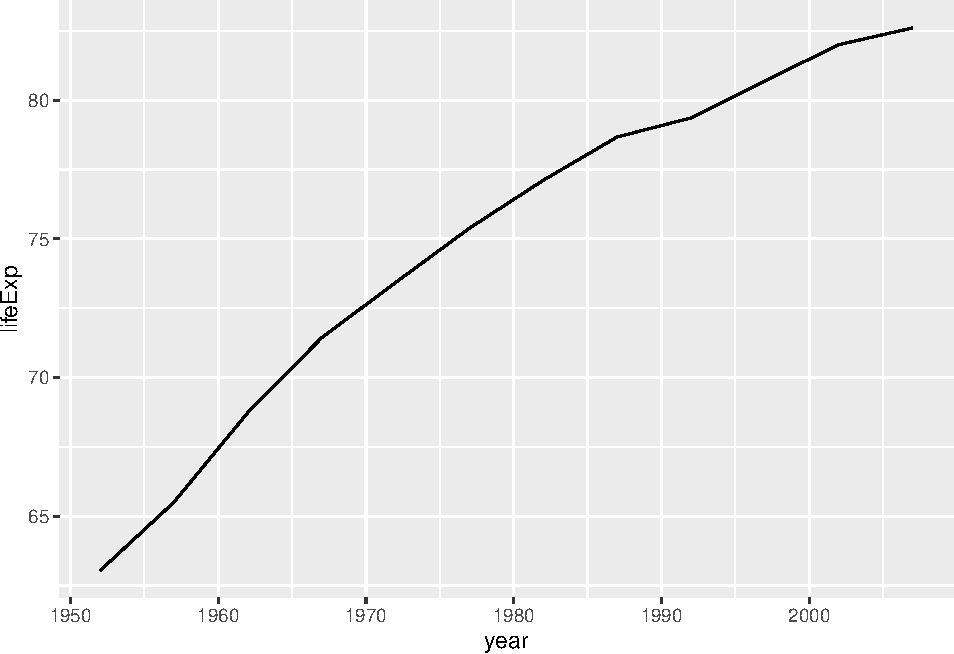
\includegraphics{BookR_files/figure-latex/unnamed-chunk-130-1.pdf}

\hypertarget{agregar-muxe1s-luxedneas}{%
\subsection{Agregar más líneas}\label{agregar-muxe1s-luxedneas}}

Hasta ahora solo nos hemos centrado en líneas simples, pero ¿qué pasa si tenemos varios países en el conjunto de datos y queremos diferenciarlos de alguna manera?

Los gráficos de líneas a menudo se amplían y se utilizan para comparar dos o más líneas. Los gráficos de líneas múltiples muestran las diferencias absolutas entre las observaciones, pero también cómo las trayectorias específicas se relacionan entre sí. Por ejemplo, respondamos a la pregunta: \emph{¿Cómo ha cambiado la esperanza de vida en los países Austria y Hungría a lo largo del tiempo?}

Primero filtramos el conjunto de datos para ambos países de interés. Luego, establecemos la variable \texttt{country} como argumento de \texttt{group} para el mapeo estético. El argumento de grupo le dice a ggplot qué observaciones pertenecen juntas y deben conectarse a través de líneas. Al especificar la variable \texttt{country}, ggplot crea una línea separada para cada país. Para que las líneas sean más fáciles de distinguir, también asignamos \texttt{color} a \texttt{country} para que cada línea de país tenga un color diferente.

\begin{Shaded}
\begin{Highlighting}[]
\NormalTok{gapminder\_comparison }\OtherTok{\textless{}{-}} 
  \FunctionTok{filter}\NormalTok{(gapminder, country }\SpecialCharTok{\%in\%} \FunctionTok{c}\NormalTok{(}\StringTok{"Austria"}\NormalTok{, }\StringTok{"Hungary"}\NormalTok{))}

\FunctionTok{ggplot}\NormalTok{(}\AttributeTok{data =}\NormalTok{ gapminder\_comparison) }\SpecialCharTok{+} 
  \FunctionTok{geom\_line}\NormalTok{(}\AttributeTok{mapping =} \FunctionTok{aes}\NormalTok{(}\AttributeTok{x =}\NormalTok{ year, }\AttributeTok{y =}\NormalTok{ lifeExp, }
                          \AttributeTok{group =}\NormalTok{ country, }
                          \AttributeTok{color =}\NormalTok{ country)}
\NormalTok{            )}
\end{Highlighting}
\end{Shaded}

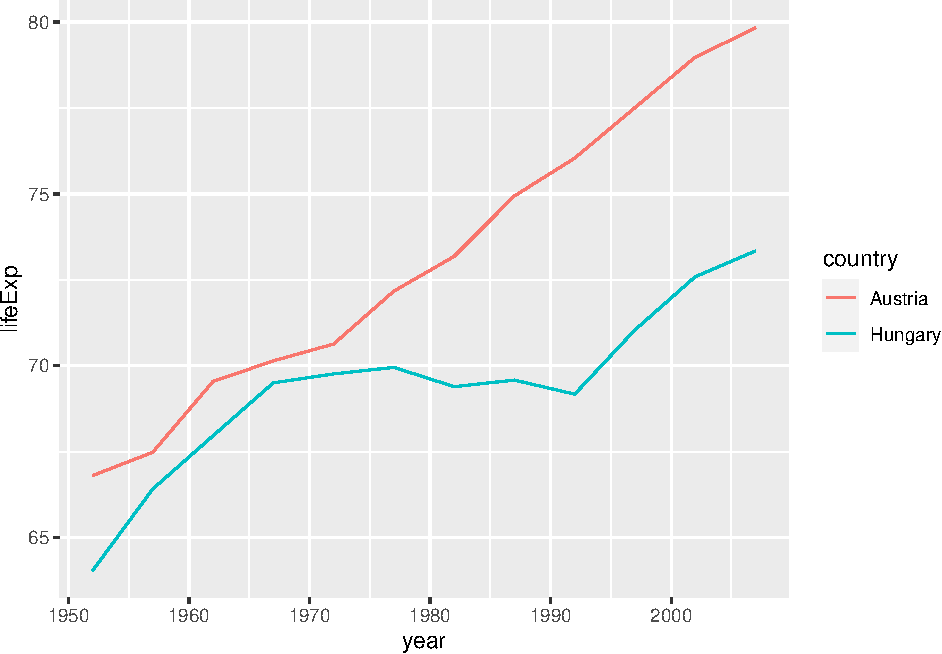
\includegraphics{BookR_files/figure-latex/unnamed-chunk-131-1.pdf}

Tenga en cuenta que ggplot también separa las líneas correctamente si solo se especifica la asignación \texttt{color} (el parámetro \texttt{group} se establece implícitamente).

\hypertarget{crea-tu-primer-gruxe1fico-de-barras}{%
\section{Crea tu primer gráfico de barras}\label{crea-tu-primer-gruxe1fico-de-barras}}

\begin{itemize}
\tightlist
\item
  Crea tu primer gráfico de barras usando \texttt{geom\_col()}
\item
  Rellenar barras con color usando la estética \texttt{fill}
\end{itemize}

\begin{verbatim}
ggplot(___) + 
  geom_col(
    mapping = aes(x = ___, y = ___, 
                  fill = ___)
 )
\end{verbatim}

\hypertarget{introducciuxf3n-a-los-gruxe1ficos-de-barras}{%
\subsection{Introducción a los gráficos de barras}\label{introducciuxf3n-a-los-gruxe1ficos-de-barras}}

Los gráficos de barras visualizan valores \texttt{numéricos} agrupados por categorías. Cada categoría está representada por una barra con una altura definida por cada valor \texttt{numérico}.

Los gráficos de barras son adecuados para comparar valores entre diferentes grupos, p.~Ej. número de votos por partidos, número de personas en diferentes países o PIB per cápita en diferentes países. Los gráficos de barras son un poco espaciosos y funcionan mejor si el número de grupos a comparar es bastante pequeño.

A continuación, puede encontrar un ejemplo que muestra la cantidad de personas (en millones) en los cinco países más grandes por población en 2007:

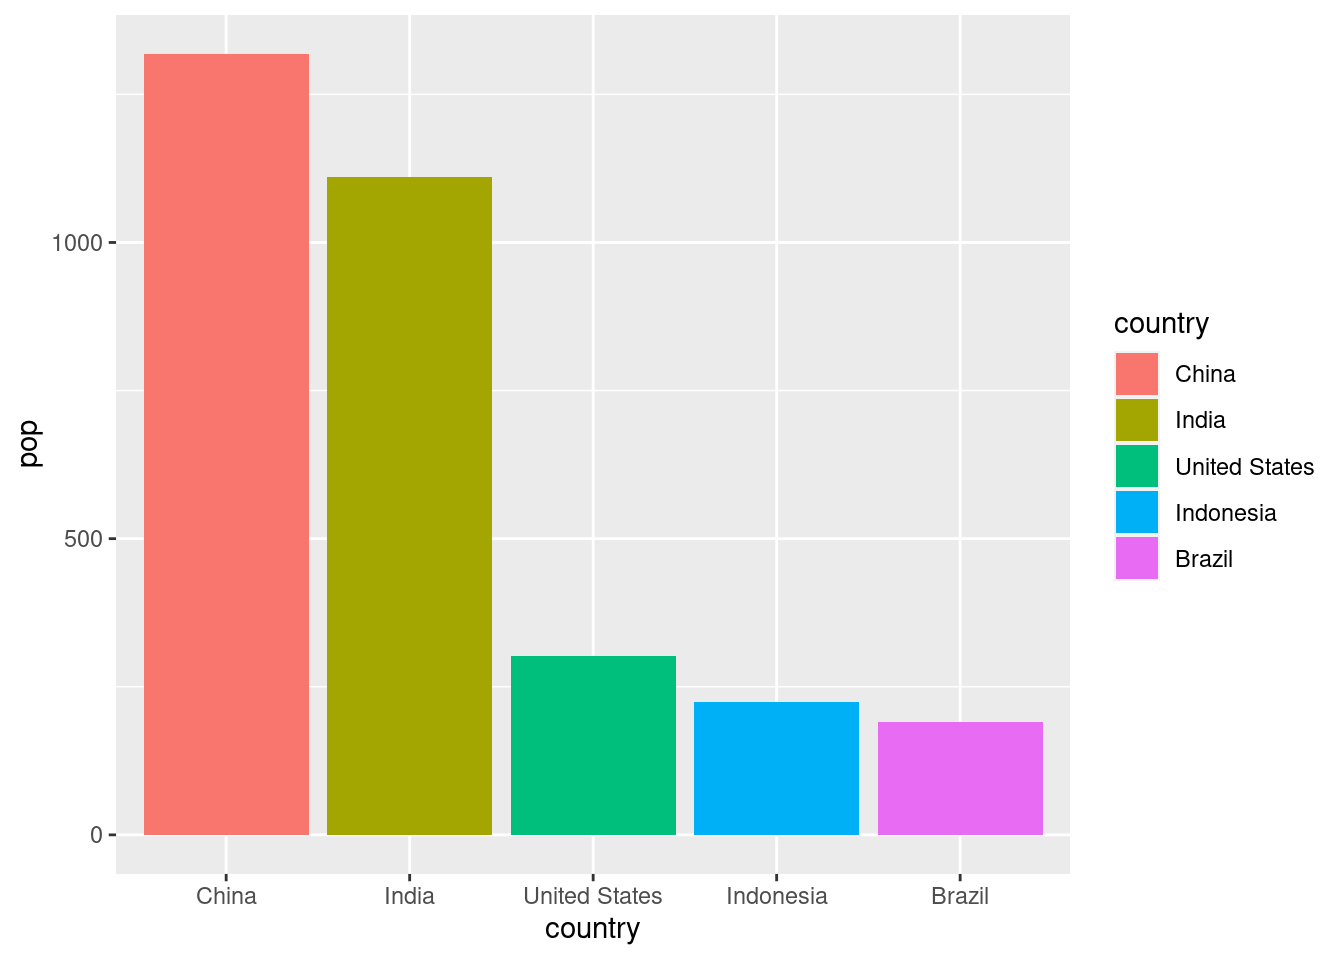
\includegraphics{img/bar1.png}

\hypertarget{crear-un-gruxe1fico-de-barras-simple}{%
\subsection{Crear un gráfico de barras simple}\label{crear-un-gruxe1fico-de-barras-simple}}

En \textbf{ggplot2}, los gráficos de barras se crean utilizando la capa geométrica \texttt{geom\_col()}. La capa \texttt{geom\_col()} requiere el mapeo estético \texttt{x} que define las diferentes barras a trazar. La altura de cada barra está definida por la variable especificada en el mapeo estético \texttt{y}. Ambas asignaciones, \texttt{x} e \texttt{y}, son necesarias para \texttt{geom\_col()}.

Creemos nuestro primer gráfico de barras con el conjunto de datos \texttt{gapminder\_top5}. Contiene datos de población (en millones) y esperanza de vida de los países más grandes por población en 2007.

\begin{Shaded}
\begin{Highlighting}[]
\NormalTok{gapminder\_top5 }\OtherTok{\textless{}{-}}\NormalTok{ gapminder }\SpecialCharTok{\%\textgreater{}\%}
  \FunctionTok{filter}\NormalTok{(year }\SpecialCharTok{==} \DecValTok{2007}\NormalTok{) }\SpecialCharTok{\%\textgreater{}\%}
  \FunctionTok{slice\_max}\NormalTok{(pop, }\AttributeTok{n=}\DecValTok{5}\NormalTok{)}
\end{Highlighting}
\end{Shaded}

\begin{Shaded}
\begin{Highlighting}[]
\FunctionTok{ggplot}\NormalTok{(gapminder\_top5) }\SpecialCharTok{+} 
  \FunctionTok{geom\_col}\NormalTok{(}\FunctionTok{aes}\NormalTok{(}\AttributeTok{x =}\NormalTok{ country, }\AttributeTok{y =}\NormalTok{ pop))}
\end{Highlighting}
\end{Shaded}

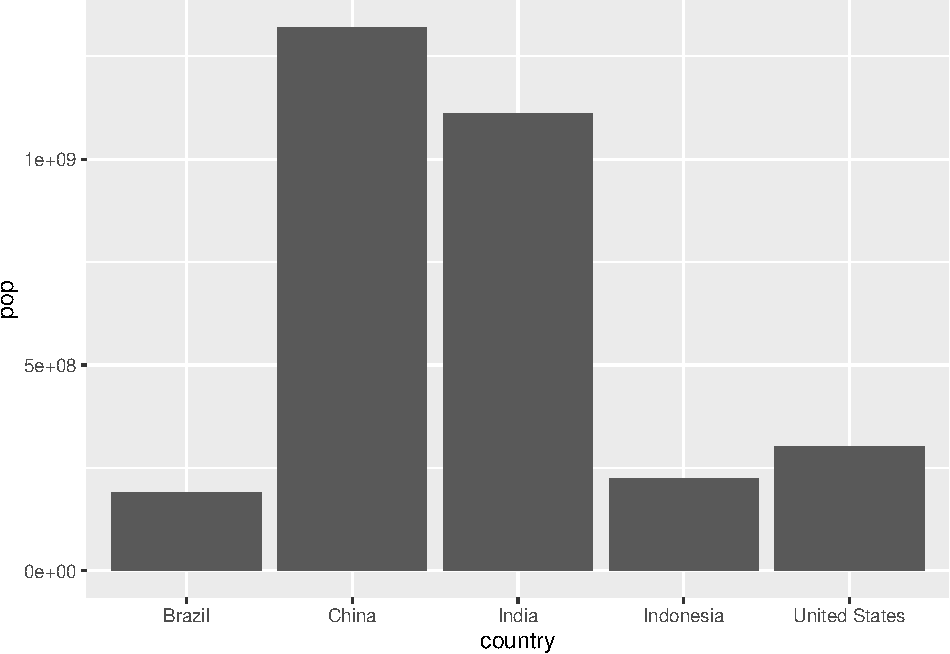
\includegraphics{BookR_files/figure-latex/unnamed-chunk-133-1.pdf}

Vemos que las barras resultantes están ordenadas por los nombres de los países en orden alfabético por defecto.

\hypertarget{llenado-de-barras-de-color}{%
\subsection{Llenado de barras de color}\label{llenado-de-barras-de-color}}

Al igual que otras geoms, \texttt{geom\_col()} permite a los usuarios asignar variables de conjuntos de datos adicionales al atributo de color de la barra. La estética \texttt{fill} se puede utilizar para llenar de color todas las barras. Una confusión habitual es la estética \texttt{color} que especifica el color de la \emph{línea} del borde de cada barra en lugar del color \texttt{fill}.

Según el conjunto de datos \texttt{gapminder\_top5}, trazamos la población (en millones) de los países más grandes y usamos la variable \texttt{continent} para colorear cada barra:

\begin{Shaded}
\begin{Highlighting}[]
\FunctionTok{ggplot}\NormalTok{(gapminder\_top5) }\SpecialCharTok{+} 
  \FunctionTok{geom\_col}\NormalTok{(}\FunctionTok{aes}\NormalTok{(}\AttributeTok{x =}\NormalTok{ country, }\AttributeTok{y =}\NormalTok{ pop, }\AttributeTok{fill =}\NormalTok{ continent))}
\end{Highlighting}
\end{Shaded}

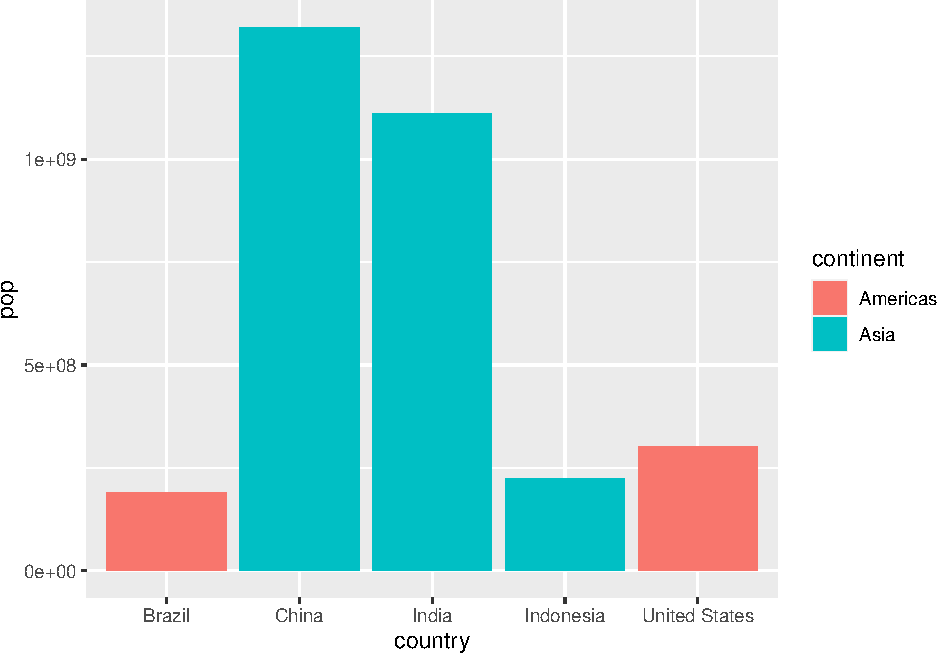
\includegraphics{BookR_files/figure-latex/unnamed-chunk-134-1.pdf}

Dado que la variable \texttt{continent} es una variable categórica, las barras tienen un esquema de color claro para cada continente. Veamos qué sucede si usamos una variable \texttt{numérica} como la esperanza de vida \texttt{lifeExp} en su lugar:

\begin{Shaded}
\begin{Highlighting}[]
\FunctionTok{ggplot}\NormalTok{(gapminder\_top5) }\SpecialCharTok{+} 
  \FunctionTok{geom\_col}\NormalTok{(}\FunctionTok{aes}\NormalTok{(}\AttributeTok{x =}\NormalTok{ country, }\AttributeTok{y =}\NormalTok{ pop, }\AttributeTok{fill =}\NormalTok{ lifeExp))}
\end{Highlighting}
\end{Shaded}

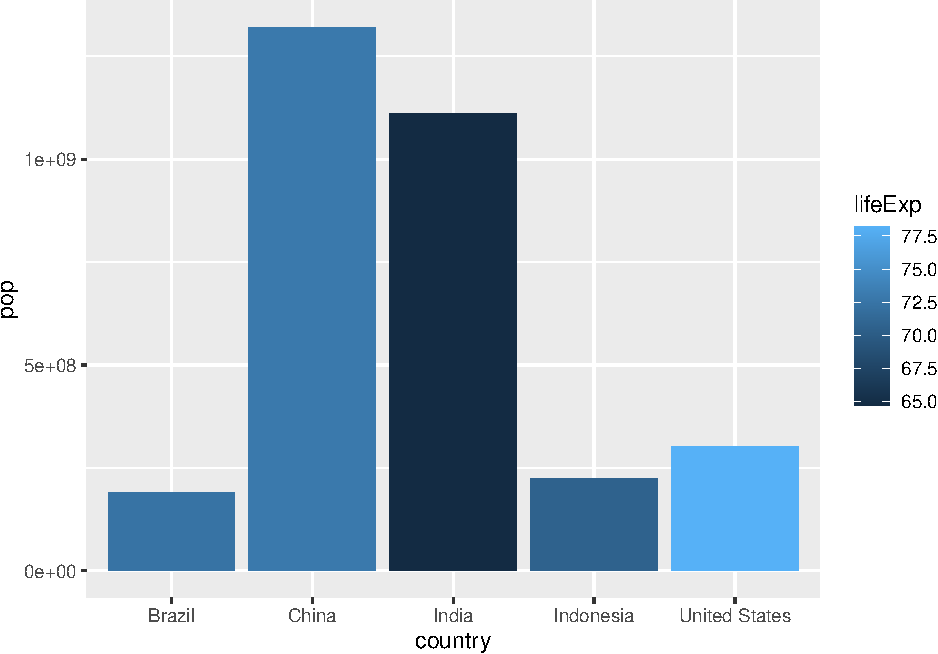
\includegraphics{BookR_files/figure-latex/unnamed-chunk-135-1.pdf}

Los colores de las barras ahora han cambiado según la leyenda \textbf{continua} de la derecha. Vemos que también se pueden utilizar variables \texttt{numéricas} para \texttt{rellenar} barras.

\hypertarget{gruxe1ficos-de-barras-apiladas}{%
\subsection{Gráficos de barras apiladas}\label{gruxe1ficos-de-barras-apiladas}}

En algunas circunstancias, puede resultar útil trazar múltiples variables de valores numéricos dentro de cada barra. Los ejemplos son valores numéricos que describen una entidad específica (por ejemplo, clientes) dividida entre varias categorías (segmentos de clientes) de modo que la altura de la barra representa el número total (todos los clientes).

El siguiente gráfico muestra la cantidad de teléfonos (en miles) por continente desde 1956 hasta 1961 como un gráfico de barras apiladas:

\begin{Shaded}
\begin{Highlighting}[]
\DocumentationTok{\#\# Ordenando la base de dato}
\NormalTok{world\_phones }\OtherTok{\textless{}{-}}\NormalTok{ WorldPhones }\SpecialCharTok{\%\textgreater{}\%}
  \FunctionTok{as.data.frame}\NormalTok{() }\SpecialCharTok{\%\textgreater{}\%}
  \FunctionTok{rownames\_to\_column}\NormalTok{(}\StringTok{"Year"}\NormalTok{) }\SpecialCharTok{\%\textgreater{}\%}
  \FunctionTok{pivot\_longer}\NormalTok{(}\AttributeTok{cols=}\SpecialCharTok{{-}}\NormalTok{Year, }\AttributeTok{names\_to=}\StringTok{"region"}\NormalTok{, }\AttributeTok{values\_to=}\StringTok{"phones"}\NormalTok{) }\SpecialCharTok{\%\textgreater{}\%}
  \FunctionTok{filter}\NormalTok{(Year }\SpecialCharTok{\textgreater{}}\DecValTok{1955}\NormalTok{)}
\end{Highlighting}
\end{Shaded}

\begin{Shaded}
\begin{Highlighting}[]
\FunctionTok{ggplot}\NormalTok{(world\_phones) }\SpecialCharTok{+} 
  \FunctionTok{geom\_col}\NormalTok{(}\FunctionTok{aes}\NormalTok{(}\AttributeTok{x =}\NormalTok{ Year, }\AttributeTok{y =}\NormalTok{ phones,}
               \AttributeTok{fill =}\NormalTok{ region))}
\end{Highlighting}
\end{Shaded}

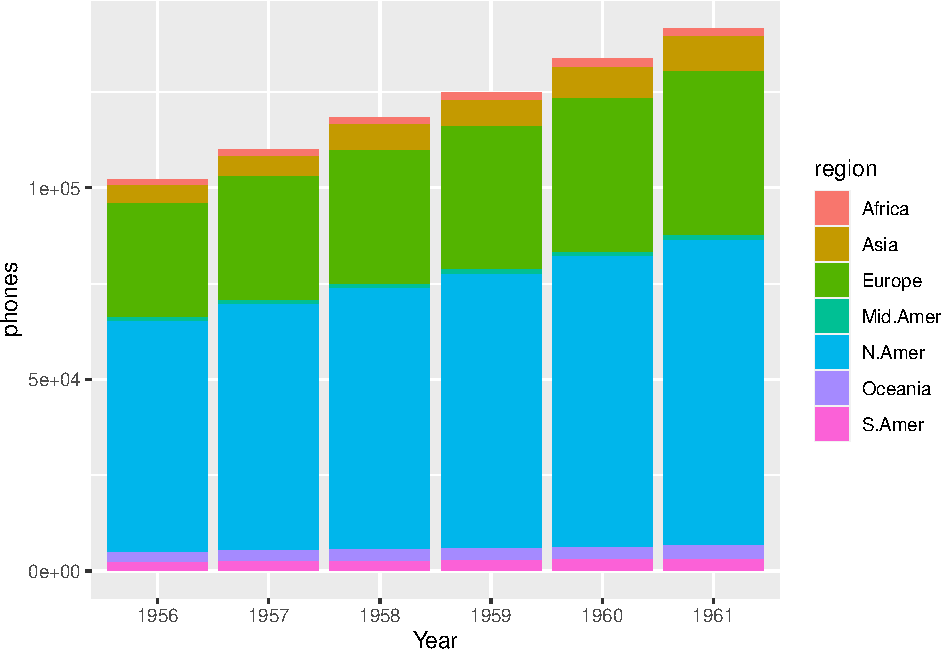
\includegraphics{BookR_files/figure-latex/unnamed-chunk-137-1.pdf}

\hypertarget{introducciuxf3n-a-machine-learning}{%
\chapter{Introducción a Machine Learning}\label{introducciuxf3n-a-machine-learning}}

Aprenda los fundamentos del aprendizaje automático, incluidos casos de uso y diferentes técnicas de aprendizaje. Diferenciar entre regresión y clasificación.

¿Qué es Machine Learning?

En los últimos años, términos como inteligencia artificial, aprendizaje automático y aprendizaje profundo se han utilizado mucho. Tan misteriosas como suenan estas palabras, ¿cuál es su diferencia y de qué son capaces?

\begin{itemize}
\tightlist
\item
  Diferenciar entre inteligencia artificial, aprendizaje automático y aprendizaje profundo
\item
  Identificar casos de uso de Machine Learning
\end{itemize}


\includegraphics{img/int.png}

\hypertarget{inteligencia-artificial}{%
\section{Inteligencia artificial}\label{inteligencia-artificial}}

La \textbf{inteligencia artificial (IA)} es la inteligencia demostrada por las máquinas, en contraste con la inteligencia natural asociada con los humanos. Por inteligencia, generalmente nos referimos a la resolución de problemas y tareas complejos, que aparentemente requieren algún tipo de habilidades cognitivas. La inteligencia artificial comenzó como una disciplina académica en la década de 1950 con el supuesto de que las computadoras pueden imitar el complejo razonamiento dentro del cerebro humano. Este campo también se conoce como \emph{inteligencia artificial general (AGI)} y el objetivo de alcanzar una inteligencia similar a la humana, incluso hoy, parece estar fuera de alcance.

Sin embargo, surgió un subcampo llamado aprendizaje automático \emph{machine learning (ML)} que se centra en problemas más específicos, como el reconocimiento de imágenes o la comprensión del lenguaje. Gracias a las aplicaciones de la industria, el aprendizaje automático se ha vuelto cada vez más popular y atrae a investigadores e inversores a nivel mundial.

\hypertarget{machine-learning-aprendizaje-automuxe1tico}{%
\section{Machine Learning (Aprendizaje automático)}\label{machine-learning-aprendizaje-automuxe1tico}}

El \textbf{machine learning (ML)} es un subcampo de la inteligencia artificial. Su objetivo es construir y aplicar modelos sofisticados sin la necesidad de reglas e instrucciones codificadas. En cambio, los modelos pueden extraer reglas y patrones de los datos y aplicarlos para nuevos problemas.

La recopilación de datos, la anotación y el procesamiento previo son requisitos previos esenciales para crear modelos de aprendizaje automático. Como regla general, cuanto mayor es la complejidad de un modelo, normalmente se necesitan más datos para el entrenamiento y la validación.

Por ejemplo, podría pensar en asistentes virtuales avanzados, como \href{https://developer.amazon.com/alexa}{Alexa} (Amazon) o \href{https://www.apple.com/siri}{Siri} (Apple), que aplican el aprendizaje automático para interpretar el lenguaje natural y predecir la mejor respuesta o reacción.

\hypertarget{aprendizaje-profundo-deep-learning}{%
\section{Aprendizaje profundo (Deep Learning)}\label{aprendizaje-profundo-deep-learning}}

El \textbf{aprendizaje profundo} es un área del aprendizaje automático, que cubre únicamente las redes neuronales. El nombre de red neuronal se inspiró en el hecho de que la arquitectura modela libremente el cerebro humano. Esta técnica demostró ser especialmente adecuada para ciertas tareas como el reconocimiento de imágenes, que es la piedra angular de aplicaciones como los vehículos autónomos.

Las redes neuronales profundas son actualmente el área de investigación más candente en toda la comunidad de IA. Su popularidad se basa en muchos avances en los últimos años, incluida la competencia ImageNet que clasifica imágenes en color de alta resolución en 1000 categorías diferentes y 1,2 (1,4) millones de muestras de entrenamiento. Las redes neuronales profundas también llevaron a avances en otras áreas en las que se desempeñaron comparables o incluso mejores que sus contrapartes humanas, incluido el reconocimiento de voz, la transcripción de escritura a mano (OCR), la traducción automática, la conducción autónoma, Go playing y muchos más.

\hypertarget{casos-de-uso-populares}{%
\section{Casos de uso populares}\label{casos-de-uso-populares}}

A medida que avanzaba el campo del aprendizaje automático y las computadoras se volvían cada vez más poderosas, se habilitaron nuevas soluciones que afectaron a casi todos los campos (científicos). Hoy en día, el aprendizaje automático ayuda a los científicos a realizar diagnósticos médicos, descubrir nuevos medicamentos, monitorear la superficie de la tierra y detectar incendios forestales, automatizar y optimizar procesos en la industria financiera, etc.

Aparte de estas aplicaciones de vanguardia, a menudo tendemos a pasar por alto que el aprendizaje automático también forma parte de nuestra vida diaria. En las siguientes secciones abordaremos estas aplicaciones de aprendizaje automático y nos centraremos en sistemas como:

\begin{itemize}
\tightlist
\item
  Sistemas de recomendación
\item
  Los motores de búsqueda
\item
  Máquina traductora
\item
  Identificación de música
\item
  Autos autónomos
\end{itemize}

\hypertarget{caso-de-uso-motores-de-buxfasqueda-y-sistemas-de-recomendaciuxf3n}{%
\subsection{Caso de uso: motores de búsqueda y sistemas de recomendación}\label{caso-de-uso-motores-de-buxfasqueda-y-sistemas-de-recomendaciuxf3n}}

Los \textbf{motores de búsqueda}, como Google, aplican el aprendizaje automático de muchas formas para brindar mejores servicios. Al escribir una consulta, por ejemplo, el aprendizaje automático proporciona sugerencias de autocompletado. Estas sugerencias se personalizan en función de los temas de tendencia actual, pero también de nuestra ubicación y búsquedas anteriores. Posteriormente, las consultas se evalúan en muchos niveles para determinar nuestras intenciones exactas y clasificar los resultados en consecuencia.

De manera similar, el aprendizaje automático determina lo que se nos recomienda en YouTube, Netflix, Amazon, etc. (un campo del aprendizaje automático, a menudo denominado \textbf{sistemas de recomendación}). Estas aplicaciones predicen nuestros intereses al analizar nuestras actividades en línea. Los artículos que hemos buscado, las películas que hemos visto, los productos que hemos comprado son todos predictores sobre nuestro comportamiento e intereses futuros.

\hypertarget{caso-de-uso-traducciuxf3n-automuxe1tica}{%
\subsection{Caso de uso: traducción automática}\label{caso-de-uso-traducciuxf3n-automuxe1tica}}

Los servicios de \textbf{traducción} como \href{https://www.deepl.com/en/translator}{DeepL} también aplican cada vez más el aprendizaje automático. La idea principal detrás de estos servicios es pasar de diccionarios simples a traductores complejos que se enfocan en el contexto e interpretan el texto como un todo. El aprendizaje automático en esta configuración se puede utilizar para crear modelos que describan cómo se expresan ciertas ideas en otros lenguajes. Esto permite una comprensión más matizada del texto escrito y proporciona traducciones más naturales. Un aspecto importante de estas soluciones es que se pueden mejorar constantemente proporcionándoles nuevos ejemplos y comentarios de los que aprender.

\hypertarget{caso-de-uso-identificaciuxf3n-de-muxfasica-y-reconocimiento-de-voz}{%
\subsection{Caso de uso: identificación de música y reconocimiento de voz}\label{caso-de-uso-identificaciuxf3n-de-muxfasica-y-reconocimiento-de-voz}}

El análisis de audio es un campo propio en el aprendizaje automático. Una herramienta común en este campo es transformar señales de audio en componentes de frecuencia. En el caso de los discos de música, la composición de estos componentes de frecuencia es tan única, que podemos definir las llamadas \emph{huellas digitales} para cada canción. Esto habilita aplicaciones de \textbf{identificación de música} como Shazam, que pueden identificar y unir canciones con precisión basándose en una muestra de solo unos segundos de duración. Del mismo modo, las aplicaciones de \textbf{reconocimiento de voz} pueden identificar fácilmente las palabras habladas y convertirlas en lenguaje escrito.

\hypertarget{caso-de-uso-coches-autuxf3nomos}{%
\subsection{Caso de uso: coches autónomos}\label{caso-de-uso-coches-autuxf3nomos}}

Los \textbf{coches autónomos} como Google Waymo y Tesla dependen en gran medida del aprendizaje automático. Al analizar los datos provenientes de varios sensores, el aprendizaje automático controla la aceleración, frenado y dirección del automóvil. Estas instrucciones se basan no solo en las normas de tráfico y las señales de tráfico, sino que incluyen un modelo predictivo continuo para evitar posibles accidentes. Aunque los modelos finales de aprendizaje automático son capaces de evaluar los datos de entrada y tomar decisiones en fracciones de segundo, el entrenamiento de los modelos requiere inmensas cantidades de datos, poder computacional y tiempo.

\hypertarget{tuxe9cnicas-de-machine-learning}{%
\section{Técnicas de Machine Learning}\label{tuxe9cnicas-de-machine-learning}}

En este capítulo

\begin{itemize}
\tightlist
\item
  Familiarízate con diferentes enfoques de machine learning
\item
  Diferenciar entre técnicas de aprendizaje supervisado, no supervisado y por refuerzo.
\item
  Vea cómo se pueden aplicar las técnicas de aprendizaje para diferentes casos de uso
\end{itemize}

La idea básica del aprendizaje automático es crear modelos que se puedan utilizar para hacer predicciones y tomar decisiones. Diferenciamos entre 3 tipos de aprendizaje automático, cada uno de ellos tiene como objetivo resolver diferentes tipos de tareas: \textbf{supervisado}, \textbf{no supervisado} y \textbf{aprendizaje reforzado}.

El \textbf{aprendizaje supervisado} tiene como objetivo aprender de un conjunto de datos de ejemplo. Nuestra suposición inicial es que el valor de un resultado conocido (por ejemplo, el cliente compra un producto) está influenciado por un conjunto de entradas medibles (edad, intereses, últimos clics). Utilizando algoritmos de aprendizaje automático, intentamos detectar y modelar estas relaciones.

El \textbf{aprendizaje no supervisado} también requiere datos de entrada, pero no existe una variable de resultado predefinida. En su lugar, tratamos de detectar patrones y establecer relaciones dentro de los datos (por ejemplo, a través de agrupaciones) o reducir dimensiones (por ejemplo, con análisis de componentes principales).

El \textbf{aprendizaje reforzado} no requiere observaciones de entrada, sino un objetivo y un entorno en el que operar. Al integrar la retroalimentación continua del entorno, esperamos que el sistema cree sus propias tácticas para lograr el objetivo.

\hypertarget{aprendizaje-supervisado}{%
\subsection{Aprendizaje supervisado}\label{aprendizaje-supervisado}}

En el \emph{aprendizaje supervisado}, la variable de resultado debe conocerse para el entrenamiento de modelos. Como ejemplo, podría pensar en un modelo para la predicción de precios de apartamentos. Este modelo podría ayudar a los agentes inmobiliarios a fijar el precio de los nuevos apartamentos que ingresan al mercado. Además, los valores previstos se pueden comparar con los precios del mercado para determinar las oportunidades de compra de los apartamentos más infravalorados. Las variables de entrada requeridas para este problema probablemente incluirían aspectos como:

\begin{itemize}
\tightlist
\item
  \textbf{Ciudad}: Ubicación del apartamento por ciudad.
\item
  \textbf{Habitaciones}: Número de habitaciones del apartamento.
\item
  \textbf{Tamaño}: Tamaño del apartamento por metros cuadrados.
\end{itemize}

Como punto de partida, necesitamos un conjunto de datos con varios ejemplos que contengan esta información:

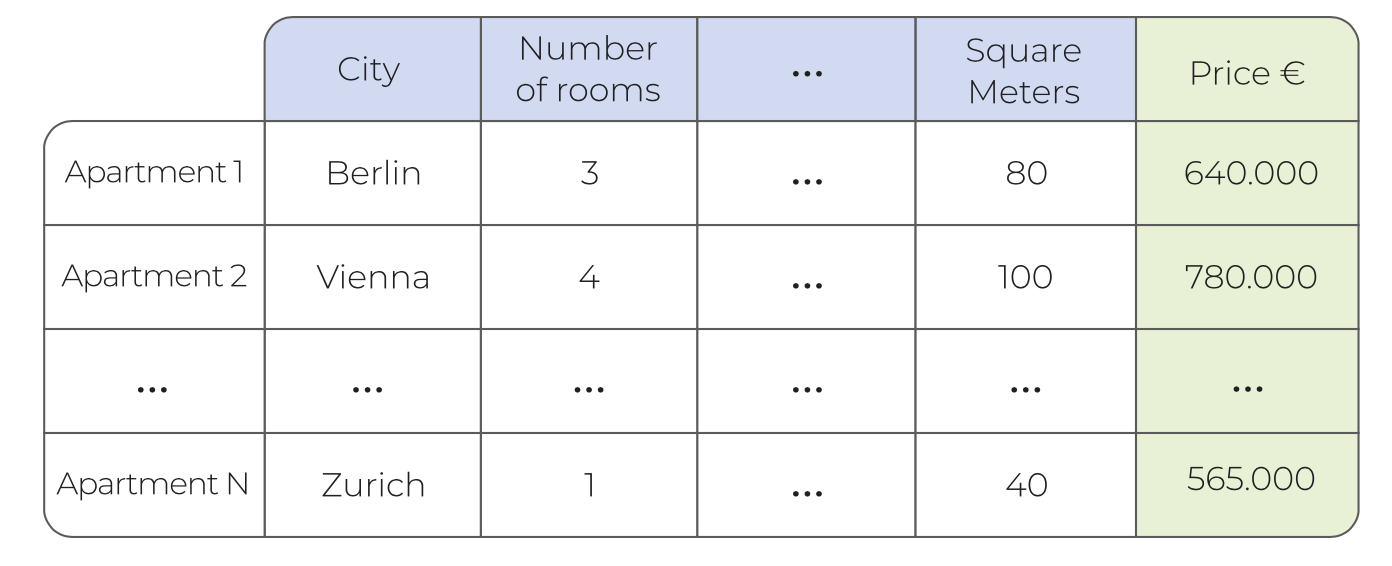
\includegraphics{img/tab1.png}

\hypertarget{aprendizaje-supervisado-objetivo}{%
\subsection{Aprendizaje supervisado: objetivo}\label{aprendizaje-supervisado-objetivo}}

El objetivo del aprendizaje automático supervisado es tomar un conjunto de ejemplos y entrenar un modelo utilizando métodos estadísticos. Este modelo debe explicar la relación entre las variables de entrada (por ejemplo, ciudad, habitaciones, tamaño) y la variable de salida (por ejemplo, precio) con la mayor precisión posible. Una vez que se ha entrenado el modelo, se puede utilizar para predecir el resultado de nuevas combinaciones de valores de entrada invisibles.

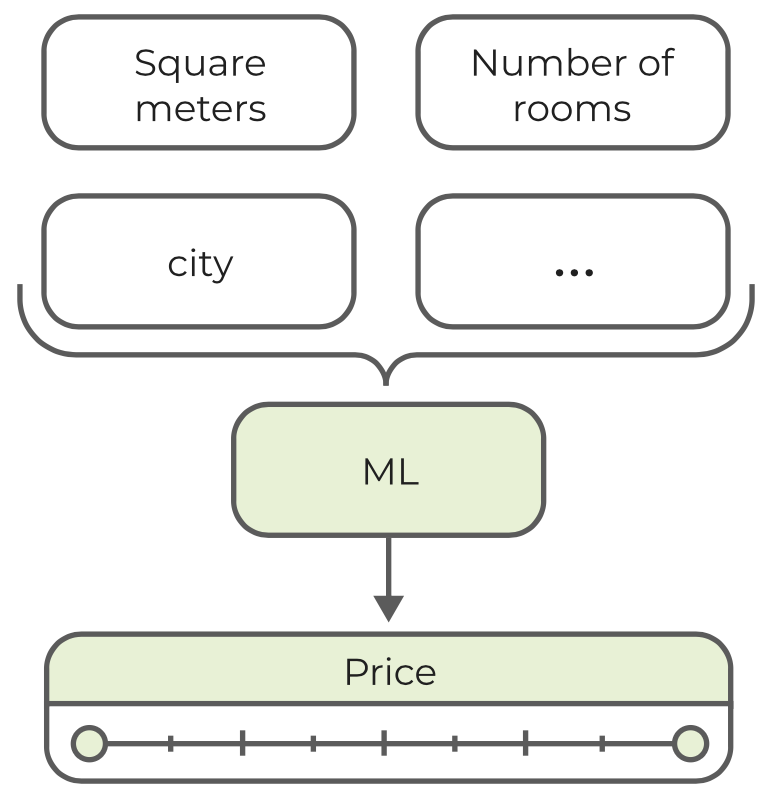
\includegraphics{img/sup.png}

\hypertarget{aprendizaje-no-supervisado}{%
\subsection{Aprendizaje no supervisado}\label{aprendizaje-no-supervisado}}

Las técnicas de aprendizaje no supervisadas extraen estructuras y patrones estadísticos de conjuntos de datos. A diferencia del aprendizaje supervisado, estas técnicas no requieren una variable de resultado predefinida en la que recibir entrenamiento.

El método de aprendizaje no supervisado más importante es la \textbf{agrupación} o cluster. La agrupación intenta agrupar las observaciones en función de su similitud. Primero, la similitud entre las observaciones se calcula como una distancia entre sí. Basándonos en estos valores, podemos determinar conglomerados (grupos) en los que las observaciones están más próximas entre sí.

\hypertarget{aprendizaje-no-supervisado-ejemplo}{%
\subsubsection{Aprendizaje no supervisado: ejemplo}\label{aprendizaje-no-supervisado-ejemplo}}

Los métodos de agrupación en clústeres se aplican a menudo como un intento de definir grupos de clientes que son similares. La similitud puede significar intereses coincidentes, datos demográficos, ubicación geográfica, etc. Esta aplicación se denomina segmentación de mercado. El objetivo de este caso de uso es comprender mejor la base de clientes y sus necesidades. Los clústeres se pueden utilizar para proporcionar anuncios y ofertas dirigidos a los clientes de acuerdo con sus propiedades. Como ejemplo, echemos un vistazo al siguiente gráfico:

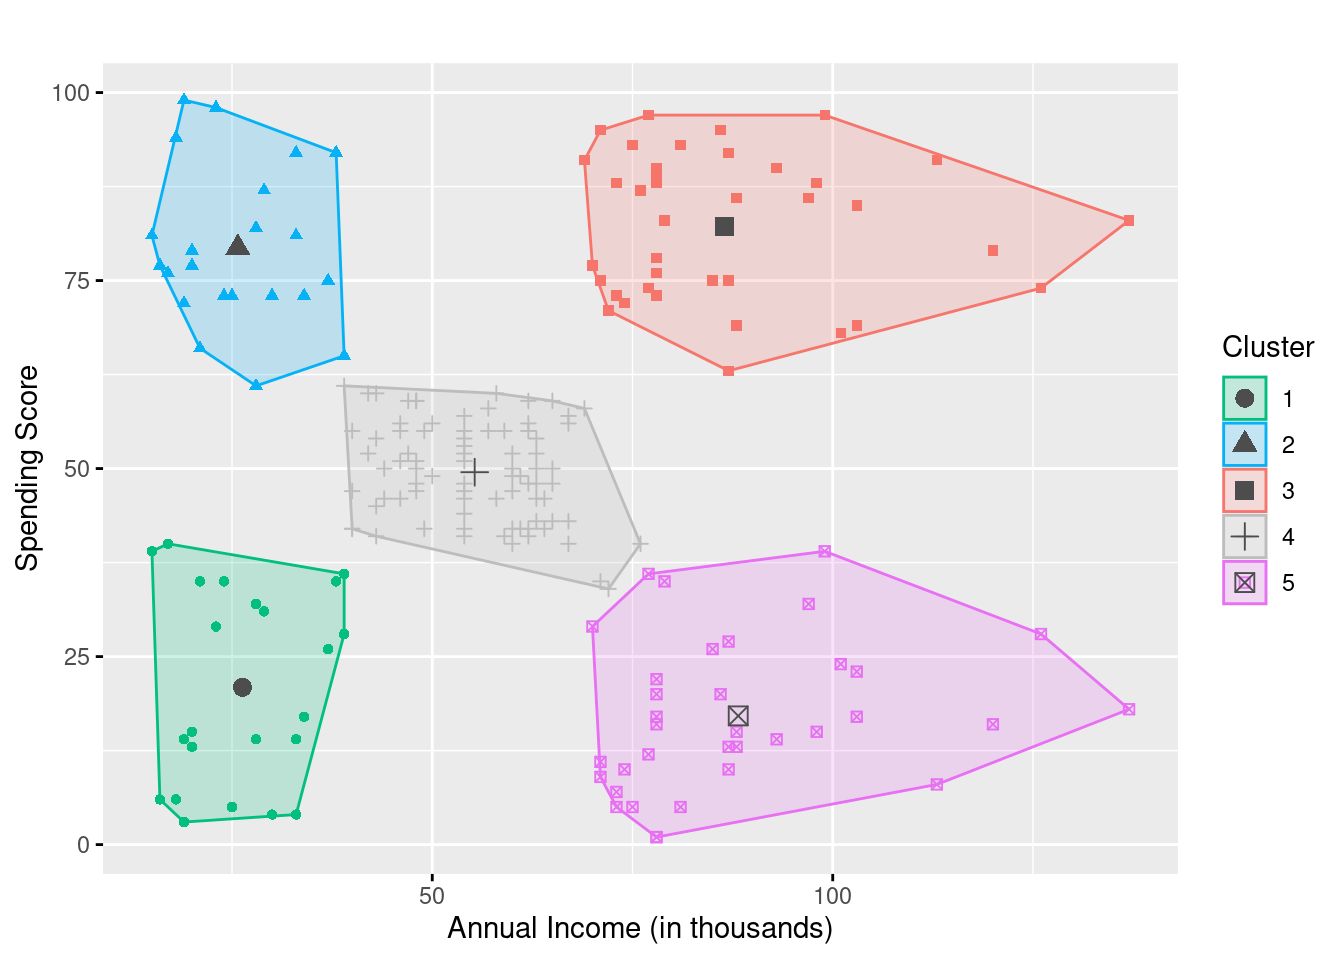
\includegraphics{img/cluster.png}
Esta gráfica compara el \texttt{Annual\ Income} y \texttt{Spending\ Score} de algunos clientes de centros comerciales. Al aplicar un algoritmo de agrupación en clústeres y definir cinco grupos, podemos separar muy bien 5 tipos diferentes de clientes. Los grupos clave en este ejemplo serían el grupo azul y rojo, que generan la mayor cantidad de ingresos. Éstos definen dos tipos de clientes. Mientras que el grupo azul contiene clientes con ingresos más bajos, el grupo rojo contiene clientes con ingresos relativamente altos. Con base en esta información, se podría adaptar la estrategia de marketing:

\begin{itemize}
\tightlist
\item
  Los clientes del clúster azul podrían ser un grupo objetivo óptimo para opciones atractivas de financiamiento y crédito.
\item
  Los clientes del grupo rojo deben mantenerse como clientes el mayor tiempo posible. En particular, debe evitarse que cambien a competidores. Por lo tanto, podrían ser un grupo objetivo óptimo para recompensas y ofertas basadas en la lealtad.
\end{itemize}

\hypertarget{aprendizaje-reforzado}{%
\subsection{Aprendizaje reforzado}\label{aprendizaje-reforzado}}

En lugar de aprender de un conjunto de ejemplos, el aprendizaje por refuerzo se basa en las recompensas acumulativas que recibe una entidad virtual (a menudo denominada \textbf{agente}) al actuar en un entorno específico. El agente intenta maximizar las recompensas acumulativas tomando decisiones. Estas decisiones se basan inicialmente en prueba y error, sin embargo, el agente se ve recompensado al tomar buenas decisiones y aprende de ellas. Del mismo modo, también existen algunos costos asociados con las malas decisiones. Por lo tanto, al crear el entorno de aprendizaje, definimos las reglas y las recompensas (y los costos), pero dejamos que el agente descubra los mejores pasos y tácticas.

\hypertarget{aprendizaje-por-refuerzo-ejemplo}{%
\subsubsection{Aprendizaje por refuerzo: ejemplo}\label{aprendizaje-por-refuerzo-ejemplo}}

Un ejemplo común es un mundo de cuadrícula, en el que el agente puede moverse de un campo a otro, excepto por posibles obstáculos o paredes, y es recompensado por encontrar la meta. Inicialmente, cada paso se daría al azar, pero después de suficientes intentos, el agente siempre iría en la dirección que maximiza sus posibilidades de obtener una recompensa. Cada paso también está asociado con un costo que reduce la recompensa acumulada. Esto significa que, desde cualquier punto de partida o posición, el agente aprendería el camino más corto hacia la recompensa después de un tiempo.

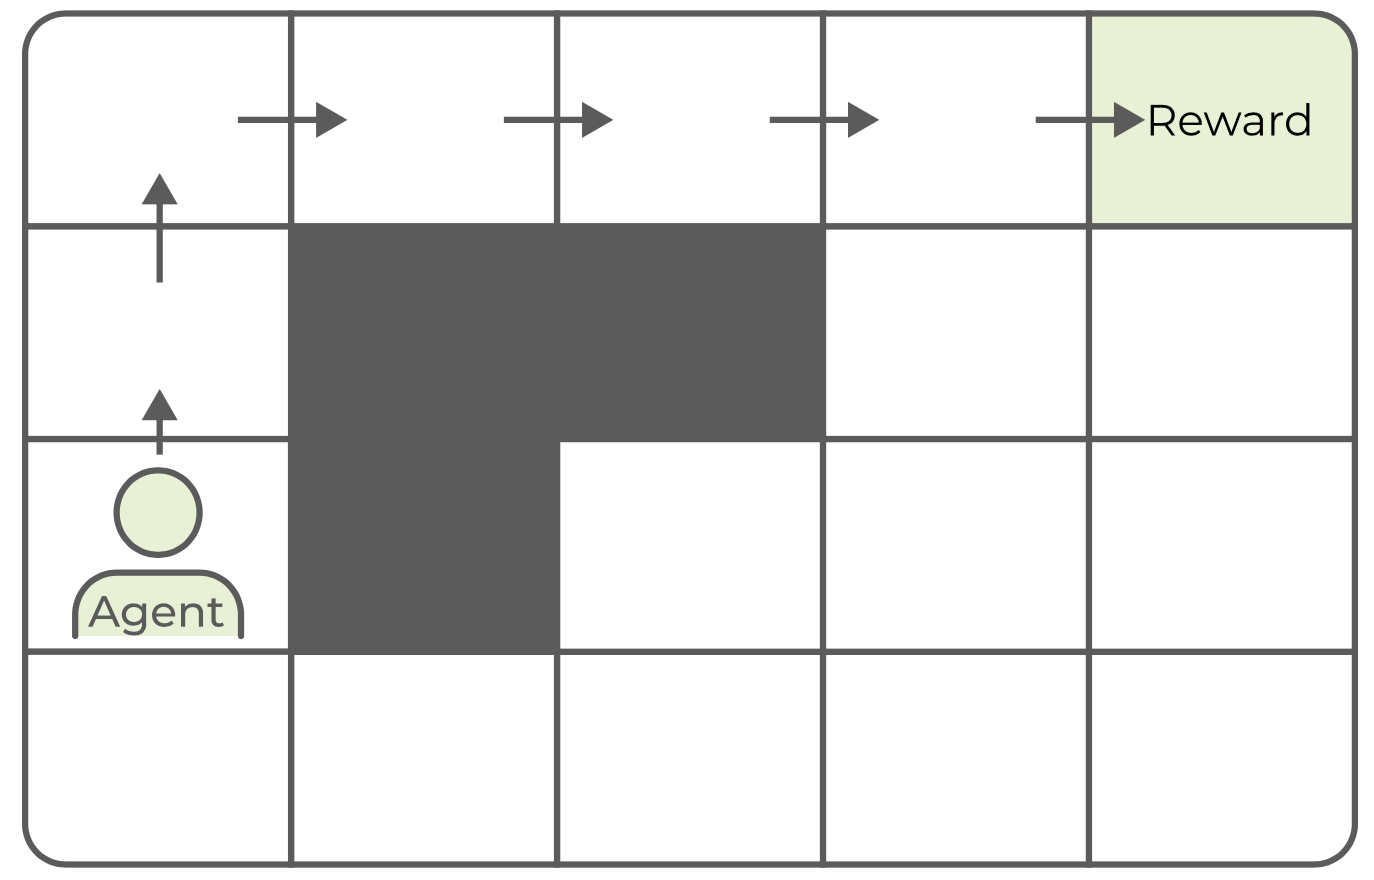
\includegraphics{img/fs.png}

\hypertarget{aprendizaje-supervisado-con-regresiuxf3n-y-clasificaciuxf3n}{%
\section{Aprendizaje supervisado con regresión y clasificación}\label{aprendizaje-supervisado-con-regresiuxf3n-y-clasificaciuxf3n}}

En el aprendizaje automático supervisado, tomamos un conjunto de observaciones con una variable de resultado conocida y entrenamos un modelo que describe con precisión la relación entre las variables de entrada y el resultado.

\begin{itemize}
\tightlist
\item
  Saber qué predictores y variables de resultado son
\item
  Diferenciar entre regresión y clasificación
\end{itemize}

\hypertarget{aprendizaje-supervisado-datos-de-entrada}{%
\subsection{Aprendizaje supervisado: datos de entrada}\label{aprendizaje-supervisado-datos-de-entrada}}

En el aprendizaje supervisado, entrenamos modelos en un conjunto de datos para describir la relación entre un valor de interés (resultado) utilizando un conjunto de valores de entrada conocidos. Por lo tanto, nuestros datos de entrenamiento para construir el modelo deben incluir todas las entradas requeridas, así como el resultado previsto en forma tabular. La tabla consta de dos partes:

\begin{enumerate}
\def\labelenumi{\arabic{enumi}.}
\tightlist
\item
  Los \textbf{predictores} o variables de entrada, que se utilizan para calcular la predicción (también conocida como matriz de modelo).
\item
  La variable de \textbf{resultado}.
\end{enumerate}

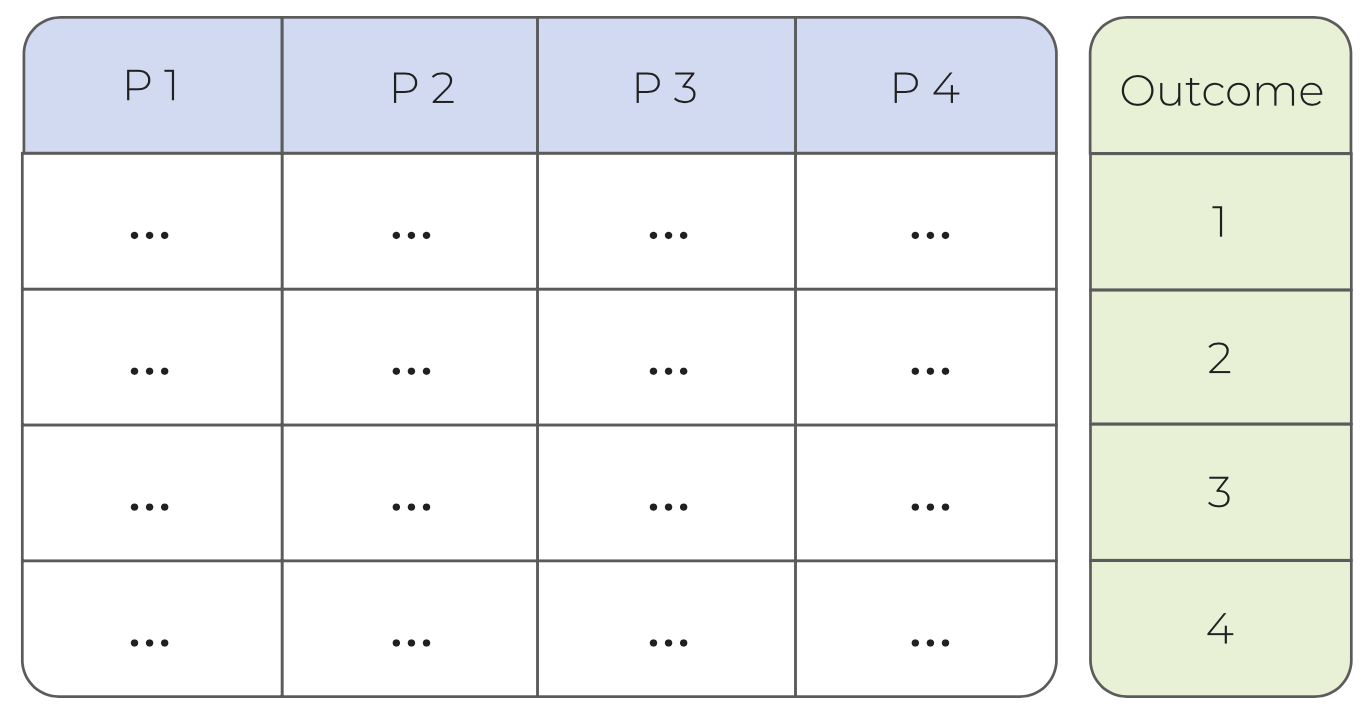
\includegraphics{img/tab.png}

\hypertarget{predictores}{%
\subsection{Predictores}\label{predictores}}

Los \textbf{predictores} son un conjunto de variables de entrada (columnas) que se utilizan para explicar y predecir el resultado. A menudo se les llama variables de \emph{entrada}, \emph{independientes}, \emph{explicativas} o simplemente \emph{características}. En el caso de los precios de los apartamentos, podría pensar en la cantidad de habitaciones, metros cuadrados o el nombre de la ciudad.

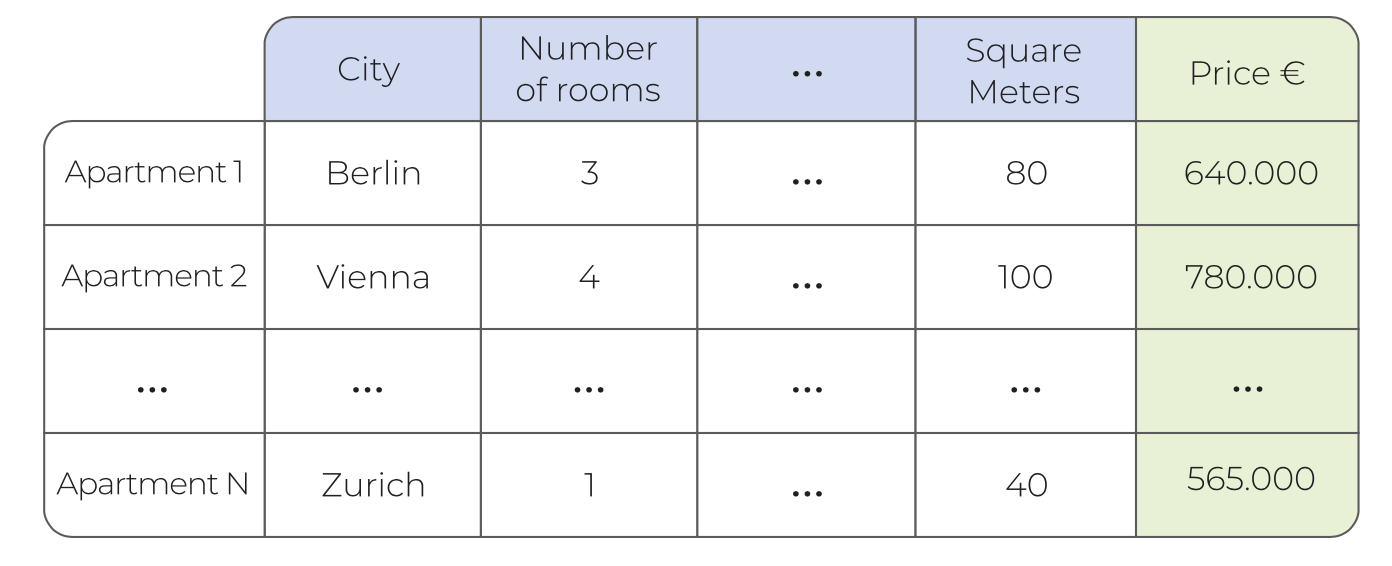
\includegraphics{img/tab1.png}

\hypertarget{variable-de-resultado}{%
\subsection{Variable de resultado}\label{variable-de-resultado}}

La variable de resultado es un solo valor/columna que queremos predecir. A menudo se la denomina \emph{objetivo}, \emph{respuesta}, \emph{variable dependiente} o simplemente denominada \emph{etiqueta}. Como ejemplo, podría pensar nuevamente en el precio de un apartamento:

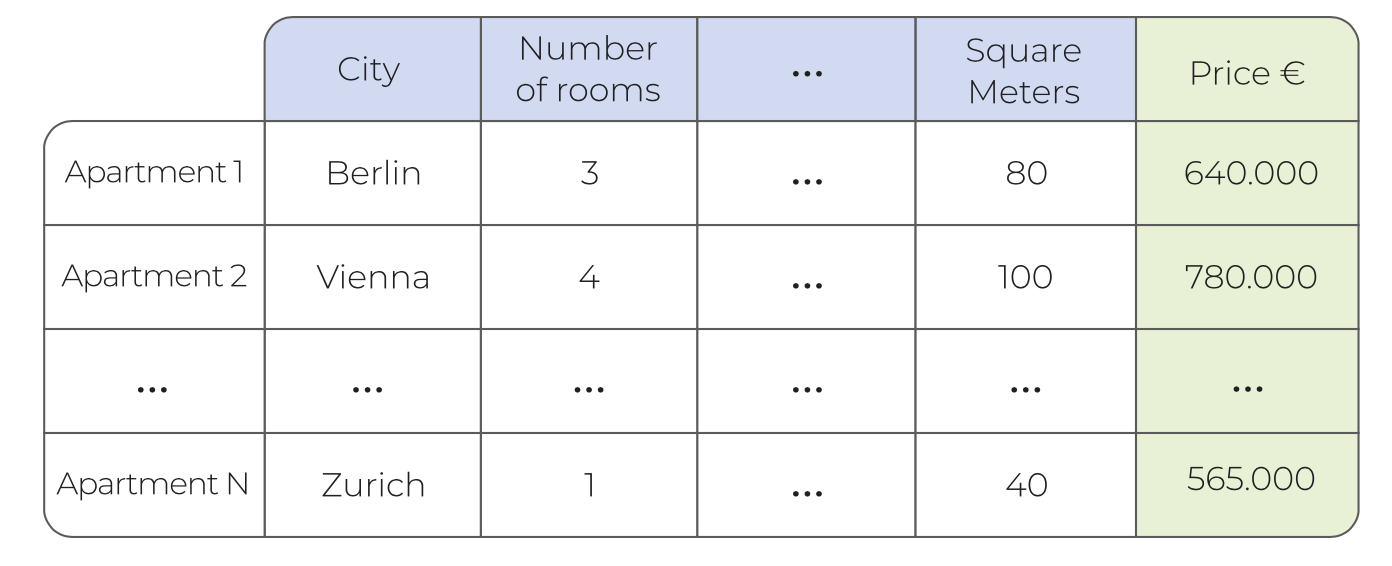
\includegraphics{img/tab1.png}

\hypertarget{regresiuxf3n-vs.-clasificaciuxf3n}{%
\subsection{Regresión vs.~clasificación}\label{regresiuxf3n-vs.-clasificaciuxf3n}}

Dentro del dominio de aprendizaje supervisado, diferenciamos entre modelos de \textbf{regresión} y de \textbf{clasificación}. El modelo específico con el que estamos tratando depende del tipo de datos de la variable de resultado. Si la variable a predecir es continua (como \texttt{numérica}), hablamos de un modelo de regresión. Si la variable es un \texttt{factor} categórico tenemos un problema de clasificación.

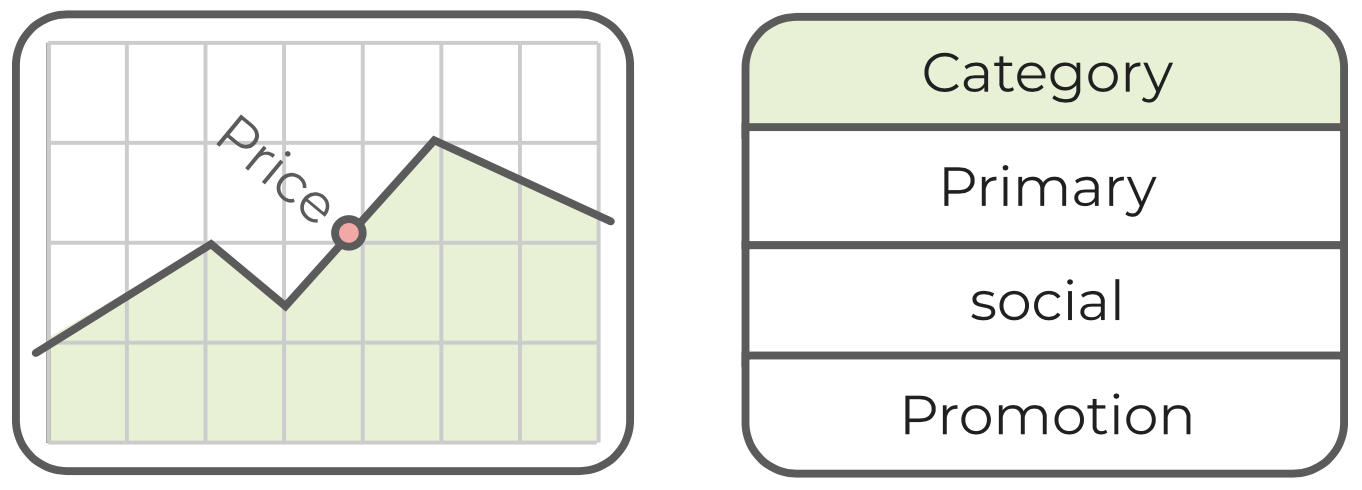
\includegraphics{img/reg.png}

\hypertarget{ejemplo-de-regresiuxf3n-vs.-clasificaciuxf3n}{%
\subsubsection{Ejemplo de regresión vs.~clasificación}\label{ejemplo-de-regresiuxf3n-vs.-clasificaciuxf3n}}

Cuando queremos predecir el precio de un apartamento, la salida es un valor \texttt{numérico} (continuo), lo que significa que estamos tratando con un modelo de regresión. Por otro lado, cuando el cliente de correo electrónico clasifica un correo electrónico en \emph{Primario}, \emph{Social} o \emph{Promociones}, el resultado es un \texttt{factor} (categórico) y necesitamos usar un modelo de clasificación.

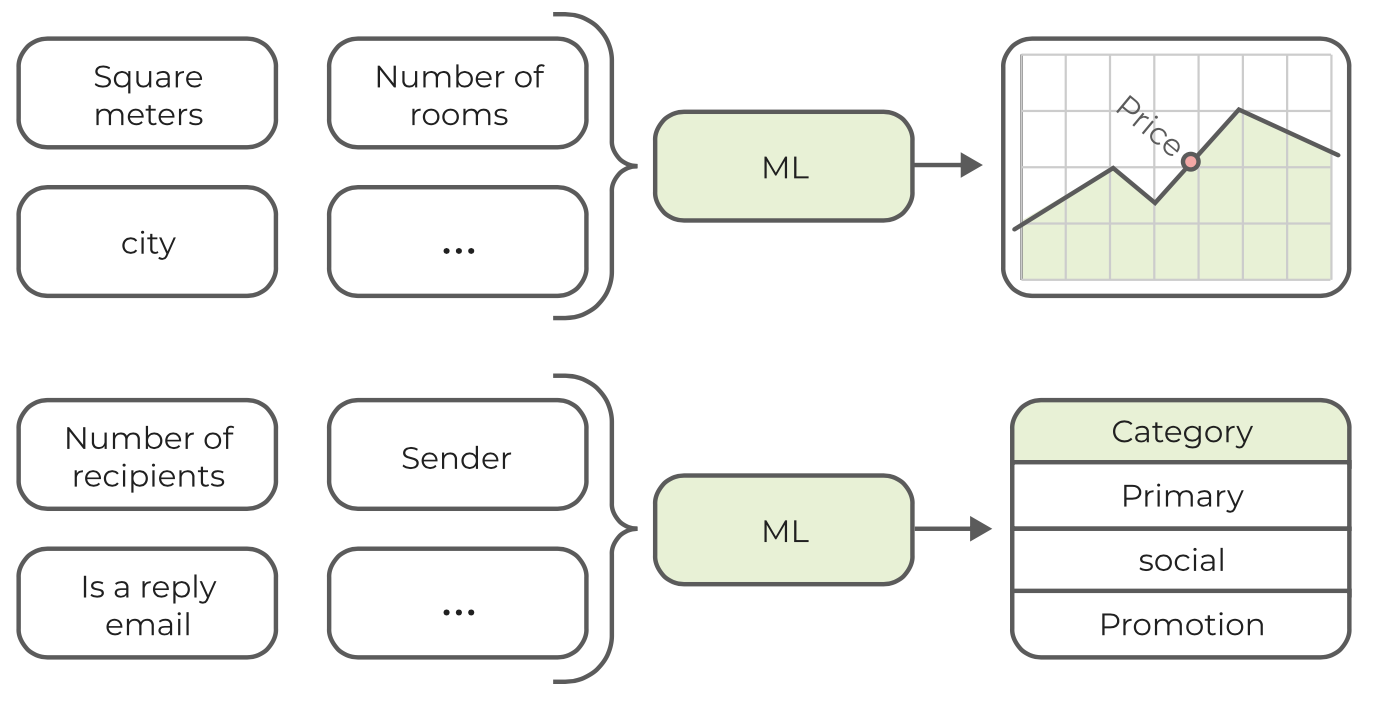
\includegraphics{img/RCE.png}

Todo el material descrito se encuentra en idioma ingles en la página oficial de Quantargo \citep{quantargo2}

  \bibliography{book.bib,packages.bib}

\end{document}
